\RequirePackage{snapshot}
% !TeX encoding = UTF-8
% !TeX spellcheck = en_GB
\documentclass[12pt,draft]{article} %taking out draft switches off marginal notes

\usepackage{incremental_SS_Translation} % all customizations in this file

\addbibresource{incremental_SS_Translation.bib}

\usepackage[record]{glossaries-extra}
\renewcommand{\glossaryname}{Glossary of Medical Substances}
\GlsXtrLoadResources % input file created by bib2gls
[% instructions to bib2gls:
src={plants}, % terms defined in plants.bib
sort={en-GB}% sort according to this locale
]

%\newglossaryentry{sample}{name={sample},
%    description={an example xxx \cite{adps}}}

\title{A Translation of the New Edition of the \SS}
\author{Jason Birch 
    \and Dominik Wujastyk 
    \and Andrey Klebanov}
\date{\texttt{Draft of \today}\\ \copyright\ Jason Birch and Dominik Wujastyk}


\includeonly{%
   00 abstract,
    01 manuscripts and editions,
    02 features of the transmission,
    translation 1-01,
    translation 1-02,
    translation 1-16,
    translation 1-28,
    translation 1-01,
    translation 5-01,
    translation 5-02,
    translation 5-03,
   translation 6-17,
  translation 6-38,
    bibliography and indexes,
    appendix,
}
\usepackage{xcolor}

\setmainfont{Libertinus Serif}



\begin{document}
   
        % Manual hyphenation points for Sanskrit words and compounds.
% By Dominik Wujastyk.
% Copyright Dominik Wujastyk 2021.
% Released under a BY-SA Creative Commons license 
% (Attribution-ShareAlike 4.0 International http://creativecommons.org/licenses/by-sa/4.0/).
% This file is still actively growing, slowly but steadily (March 2021) .
%
% These special hyphenations have to be loaded after
% \begin{document}. See
% http://www.tug.org/pipermail/xetex/2008-July/010362.html
% Or use 
% \AtBeginDocument{% Manual hyphenation points for Sanskrit words and compounds.
% By Dominik Wujastyk.
% Copyright Dominik Wujastyk 2021.
% Released under a BY-SA Creative Commons license 
% (Attribution-ShareAlike 4.0 International http://creativecommons.org/licenses/by-sa/4.0/).
% This file is still actively growing, slowly but steadily (March 2021) .
%
% These special hyphenations have to be loaded after
% \begin{document}. See
% http://www.tug.org/pipermail/xetex/2008-July/010362.html
% Or use 
% \AtBeginDocument{% Manual hyphenation points for Sanskrit words and compounds.
% By Dominik Wujastyk.
% Copyright Dominik Wujastyk 2021.
% Released under a BY-SA Creative Commons license 
% (Attribution-ShareAlike 4.0 International http://creativecommons.org/licenses/by-sa/4.0/).
% This file is still actively growing, slowly but steadily (March 2021) .
%
% These special hyphenations have to be loaded after
% \begin{document}. See
% http://www.tug.org/pipermail/xetex/2008-July/010362.html
% Or use 
% \AtBeginDocument{\input{sanskrit-hyphenations}}% should work, but doesn't
% special hyphenations for Sanskrit words tagged in
% Polyglossia.
% *English,\textenglish{},text,and
% *Sanskrit,\textsanskrit{},text.
%
% English (see below for \textsanskrit)
%
\hyphenation{%
    dhanva-ntariṇopa-diṣ-ṭaḥ
    suśruta-nāma-dheyena
    tac-chiṣyeṇa
    kāśyapa-saṃ-hitā
    cikitsā-sthāna
    su-śruta-san-dīpana-bhāṣya
    dṛṣṭi-maṇḍala
    uc-chiṅga-na
    sarva-siddhānta-tattva-cūḍā-maṇi
    tulya-sau-vīrāñja-na
    indra-gopa
    śrī-mad-abhi-nava-guptā-cārya-vi-ra-cita-vi-vṛti-same-tam
    viśva-nātha
śrī-mad-devī-bhāga-vata-mahā-purāṇa
    siddhā-n-ta-sun-dara
    brāhma-sphuṭa-siddh-ānta
    bhū-ta-saṅ-khyā
    bhū-ta-saṃ-khyā
    kathi-ta-pada
    devī-bhā-ga-vata-purāṇa
    devī-bhā-ga-vata-mahā-purāṇa
    Siddhānta-saṃ-hitā-sāra-sam-uc-caya
    sau-ra-pau-rāṇi-ka-mata-sam-artha-na
    Pṛthū-da-ka-svā-min
    Brah-ma-gupta
    Brāh-ma-sphu-ṭa-siddhānta
    siddhānta-sun-dara
    vāsa-nā-bhāṣya
    catur-veda
    bhū-maṇḍala
    jñāna-rāja
    graha-gaṇi-ta-cintā-maṇi
    Śiṣya-dhī-vṛd-dhi-da-tan-tra
    brah-māṇḍa-pu-rā-ṇa
    kūr-ma-pu-rā-ṇa
    jam-bū-dvī-pa
    bhā-ga-vata-pu-rā-ṇa
    kupya-ka
    nandi-suttam
    nandi-sutta
    su-bodhiā-bāī
    asaṅ-khyāta
    saṅ-khyāta
    saṅ-khyā-pra-māṇa
    saṃ-khā-pamāṇa
    nemi-chandra
    anu-yoga-dvāra
    tattvārtha-vārtika
    aka-laṅka
    tri-loka-sāra
    gaṇi-ma-pra-māṇa
    gaṇi-ma-ppa-māṇa
    eka-pra-bhṛti
gaṇaṇā-saṃ-khā
gaṇaṇā-saṅ-khyā
dvi-pra-bhṛti
duppa-bhi-ti-saṃ-khā
vedanābhi-ghāta
Viṣṇu-dharmottara-pu-rāṇa
abhaya-deva-sūri-vi-racita-vṛtti-vi-bhūṣi-tam
abhi-dhar-ma
abhi-dhar-ma-ko-śa
abhi-dhar-ma-ko-śa-bhā-ṣya
abhi-dharma-kośa-bhāṣya
abhi-dharma-kośa-bhāṣyam
abhi-nava
abhyaṃ-karopāhva-vāsu-deva-śāstri-vi-ra-ci-ta-yā
ācārya-śrī-jina-vijayālekhitāgra-vacanālaṃ-kṛtaś-ca
ācāry-opā-hvena
ādhāra
adhi-kāra
adhi-kāras
ādi-nātha
agni-besha
agni-veśa
ahir-budhnya
ahir-budhnya-saṃ-hitā
aita-reya-brāhma-ṇa
akusī-dasya
amara-bharati
Amar-augha-pra-bo-dha
amṛ-ta-siddhi
ānanda-kanda
ānan-da-rā-ya
ānand-āśra-ma-mudraṇā-la-ya
ānand-āśra-ma-saṃ-skṛta-granth-āva-liḥ
anna-pāna-mūlā
anu-ban-dhya-lakṣaṇa-sam-anv-itās
anu-bhav-ād
anu-bhū-ta-viṣayā-sam-pra-moṣa
anu-bhū-ta-viṣayā-sam-pra-moṣaḥ
aparo-kṣā-nu-bhū-ti
app-proxi-mate-ly
ardha-rātrika-karaṇa
ārdha-rātrika-karaṇa
ariya-pary-esana-sutta
arun-dhatī
ārya-bhaṭa
ārya-bhaṭā-cārya-vi-racitam
ārya-bhaṭīya
ārya-bhaṭīyaṃ
ārya-lalita-vistara-nāma-mahā-yāna-sūtra
ārya-mañju-śrī-mūla-kalpa
ārya-mañju-śrī-mūla-kalpaḥ
asaṃ-pra-moṣa
aṣṭāṅga-hṛdaya-saṃ-hitā
aṣṭāṅga-saṃ-graha
asura-bhavana
aśva-ghoṣa
ātaṅka-darpaṇa-vyā-khyā-yā
atha-vā
ava-sāda-na
āyār-aṅga-suttaṃ
ayur-ved
ayur-veda
āyur-veda
āyur-veda-dīpikā
āyur-veda-dīpikā-vyā-khyayā
āyur-ve-da-ra-sā-yana
āyur-veda-sū-tra
ayur-vedic
āyur-vedic
ayur-yog
bādhirya
bahir-deśa-ka
bala-bhadra
bala-kot
bala-krishnan
bāla-kṛṣṇa
bau-dhā-yana-dhar-ma-sūtra
bel-valkar
bhadra-kālī-man-tra-vi-dhi-pra-karaṇa
bhadrā-sana
bhadrā-sanam
bha-ga-vat-pāda
bhaiṣajya-ratnāvalī
bhan-d-ar-kar
bhartṛhari-viracitaḥ
bhaṭṭā-cārya
bhaṭṭot-pala-vi-vṛti-sahitā
Bhiṣag-varāḍha-malla-vi-racita-dīpikā-Kāśī-rāma-vaidya-vi-raci-ta-gūḍhā-rtha-dīpikā-bhyāṃ
bhiṣag-varāḍha-malla-vi-racita-dīpikā-Kāśī-rāma-vaidya-vi-racita-gūḍhārtha-dīpikā-bhyāṃ
bhoja-deva-vi-raci-ta-rāja-mārtaṇḍā-bhi-dha-vṛtti-sam-e-tāni
bhu--va-na-dī-pa-ka
bīja-pallava
bi-kaner
bodhi-sat-tva-bhūmi
brahma-gupta
brahmā-nanda
brahmāṇḍa-mahā-purā-ṇa
brahmāṇḍa-mahā-purā-ṇam
brahma-randhra
brahma-siddh-ānta
brāhma-sphuṭa-siddh-ānta
brāhma-sphu-ṭa-siddhānta
brahma-vi-hāra
brahma-vi-hāras
brahma-yā-mala-tan-tra
Bra-ja-bhāṣā
bṛhad-āraṇya-ka
bṛhad-yā-trā
bṛhad-yogi-yājña-valkya-smṛti
bṛhad-yogī-yājña-valkya-smṛti
bṛhaj-jāta-kam
bṛhat-khe-carī-pra-kāśa
buddhi-tattva-pra-karaṇa
cak-ra-dat-ta
cakra-datta
cakra-pāṇi-datta
cā-luk-ya
caraka-prati-saṃ-s-kṛta
caraka-prati-saṃ-s-kṛte
caraka-saṃ-hitā
casam-ul-lasi-tāmaharṣiṇāsu-śrutenavi-raci-tāsu-śruta-saṃ-hitā
cau-kham-ba
cau-luk-yas
chandi-garh
chara-ka
cha-rīre
chatt-opa-dh-ya-ya
chau-kham-bha
chi-ki-tsi-ta
cid-ghanā-nanda-nātha
ci-ka-ner
com-men-taries
com-men-tary
com-pre-hen-sive-ly
daiva-jñālaṃ-kṛti
daiva-jñālaṅ-kṛti
dāmo-dara-sūnu-Śārṅga-dharācārya-vi-racitā
Dāmodara-sūnu-Śārṅga-dharācārya-vi-racitā
darśanā-ṅkur-ābhi-dhayā
das-gupta
deha-madhya
deha-saṃ-bhava-hetavaḥ
deva-datta
deva-nagari
deva-nāgarī
devā-sura-siddha-gaṇaiḥ
dha-ra-ni-dhar
dharma-megha
dharma-meghaḥ
dhru-vam
dhru-va-sya
dhru-va-yonir
dhyā-na-grahopa-deśā-dhyā-yaś
dṛḍha-śūla-yukta-rakta
dvy-ulbaṇaikolba-ṇ-aiḥ
four-fold
gan-dh-ā-ra
gārgīya-jyoti-ṣa
gārgya-ke-rala-nīla-kaṇṭha-so-ma-sutva-vi-racita-bhāṣyo-pe-tam
garuḍa-mahā-purāṇa
gaurī-kāñcali-kā-tan-tra
gau-tama
gauta-mādi-tra-yo-da-śa-smṛty-ātma-kaḥ
gheraṇḍa-saṃ-hitā
gorakṣa-śata-ka
go-tama
granth-ā-laya
grantha-mālā
gran-tha-śreṇiḥ
grāsa-pramāṇa
guru-maṇḍala-grantha-mālā
gyatso
hari-śāstrī
haṭhābhyāsa-paddhati
haṭha-ratnā-valī
Haṭha-saṅ-keta-candri-kā
haṭha-tattva-kau-mudī
haṭha-yoga
hāyana-rat-na
haya-ta-gran-tha
hema-pra-bha-sūri
hetu-lakṣaṇa-saṃ-sargād
hīna-madhyādhi-kaiś
hindī-vyā-khyā-vi-marśope-taḥ
hoern-le
ijya-rkṣa
ikka-vālaga
indra-dhvaja
indrāṇī-kalpa
indria
Īśāna-śiva-guru-deva-pad-dhati
jābāla-darśanopa-ni-ṣad
jadav-ji
jagan-nā-tha
jala-basti
jal-pa-kal-pa-tāru
jam-bū-dvī-pa-pra-jña-pti
jam-bū-dvī-pa-pra-jña-pti-sūtra
jana-pad-a-sya
jāta-ka-kar-ma-pad-dhati
jaya-siṃha
jinā-agama-grantha-mālā
jin-en-dra-bud-dhi
jīvan-muk-ti-vi-veka
jñā-na-nir-mala
jñā-na-nir-malaṃ
joga-pra-dīpya-kā
jya-rkṣe
Jyo-tiḥ-śās-tra
jyo-ti-ṣa-rāya
jyoti-ṣa-rāya
jyotiṣa-siddhānta-saṃ-graha
jyotiṣa-siddhānta-saṅ-graha
kāka-caṇḍīśvara-kal-pa-tan-tra
kakṣa-puṭa
kali-kāla-sarva-jña
kali-kāla-sarva-jña-śrī-hema-candrācārya-vi-raci-ta
kali-kāla-sarva-jña-śrī-hema-candrācārya-vi-raci-taḥ
kali-yuga
kal-pa
kal-pa-sthāna
kalyāṇa-kāraka
Kāmeśva-ra-siṃha-dara-bhaṅgā-saṃ-skṛta-viśva-vidyā-layaḥ
kapāla-bhāti
karaṇa-tilaka
kar-ma
kar-man
kāṭhaka-saṃ-hitā
kavia-rasu
kavi-raj
keśa-va-śāstrī
ke-vala--rāma
keva-la-rāma
khaṇḍa-khādyaka-tappā
khe-carī-vidyā
knowl-edge
kol-ka-ta
kriyā-krama-karī
kṛṣṇa-pakṣa
kṛtti-kā
kṛtti-kās
kubji-kā-mata-tantra
kula-pañji-kā
kul-karni
ku-māra-saṃ-bhava
kuṭi-pra-veśa
kuṭi-pra-veśika
lakṣ-mī-veṅ-kaṭ-e-ś-va-ra
lit-era-ture
lit-era-tures
locana-roga
mādha-va
mādhava-kara
mādhava-ni-dāna
mādhava-ni-dā-nam
madh-ūni
madhya
mādhyan-dina
madhye
mahā-bhāra-ta
mahā-deva
mahā-kavi-bhartṛ-hari-praṇīta-tvena
maha-mahopa-dhyaya
mahā-maho-pā-dhyā-ya-śrī-vi-jñā-na-bhikṣu-vi-raci-taṃ
mahā-mati-śrī-mādhava-kara-pra-ṇī-taṃ
mahā-mudrā
mahā-muni-śrī-mad-vyāsa-pra-ṇī-ta
mahā-muni-śrī-mad-vyāsa-pra-ṇī-taṃ
maharṣiṇā
maha-rṣi-pra-ṇīta-dharma-śāstra-saṃ-grahaḥ
Maha-rṣi-varya-śrī-yogi-yā-jña-valkya-śiṣya-vi-racitā
mahā-sacca-ka-sutta
mahā-sati-paṭṭhā-na-sutta
mahā-vra-ta
mahā-yāna-sūtrālaṅ-kāra
maitrāya-ṇī-saṃ-hitā
maktab-khānas
māla-jit
māli-nī-vijayot-tara-tan-tra
manaḥ-sam-ā-dhi
mānasol-lāsa
mānava-dharma-śāstra
mandāgni-doṣa
mannar-guḍi
mano-har-lal
mano-ratha-nandin
man-u-script
man-u-scripts
mataṅga-pārame-śvara
mater-ials
matsya-purāṇam
medh-ā-ti-thi
medhā-tithi
mithilā-stha
mithilā-stham
mithilā-sthaṃ
mṛgendra-tantra-vṛtti
mud-rā-yantr-ā-laye
muktā-pīḍa
mūla-pāṭha
muṇḍī-kalpa
mun-sh-ram
Nāda-bindū-pa-ni-ṣat
nāga-bodhi
nāga-buddhi
nakṣa-tra
nara-siṃha
nārā-yaṇa-dāsa
nārā-yaṇa-dāsa
nārā-yaṇa-kaṇṭha
nārā-yaṇa-paṇḍi-ta-kṛtā
nar-ra-tive
nata-rajan
nava-pañca-mayor
nava-re
naya-na-sukho-pā--dhyāya
ni-ban-dha-saṃ-grahā-khya-vyākhya-yā
niban-dha-san-graha
ni-dā-na
nidā-na-sthā-na-sya
ni-dāna-sthānasyaśrī-gaya-dāsācārya-vi-racitayānyāya-candri-kā-khya-pañjikā-vyā-khyayā
nir-anta-ra-pa-da-vyā-khyā
nir-guṇḍī-kalpa
nir-ṇaya-sā-gara
Nir-ṇaya-sāgara
nir-ṇa-ya-sā-gara-mudrā-yantrā-laye
nir-ṇa-ya-sā-ga-ra-yantr-āla-ya
nir-ṇaya-sā-gara-yantr-ā-laye
niśvāsa-kārikā
nīti-śṛṅgāra-vai-rāgyādi-nāmnāsamākhyā-tānāṃ
nityā-nanda
nya-grodha
nya-grodho
nyā-ya-candri-kā-khya-pañji-kā-vyā-khya-yā
nyāya-śās-tra
okaḥ-sātmya
okaḥ-sātmyam
okaḥ-sātmyaṃ
oka-sātmya
oka-sātmyam
oka-sātmyaṃ
oris-sa
oṣṭha-saṃ-puṭa
ousha-da-sala
padma-pra-bha-sūri
Padma-prā-bhṛ-ta-ka
padma-sva-sti-kārdha-candrādike
paitā-maha-siddhā-nta
pañca-karma
pañca-karman
pāñca-rātrā-gama
pañca-siddh-āntikā
paṅkti-śūla
Paraśu-rāma
paraśu-rāma
pari-likh-ya
pāśu-pata-sū-tra-bhāṣya
pātañ-jala-yoga-śās-tra
pātañ-jala-yoga-śās-tra-vi-varaṇa
pat-añ-jali
pat-na
pāva-suya
phiraṅgi-can-dra-cchedyo-pa-yogi-ka
pim-pal-gaon
pipal-gaon
pitta-śleṣ-man
pit-ta-śleṣ-ma-śoṇi-ta
pitta-śoṇi-ta
prā-cīna-rasa-granthaḥ
prā-cya
prā-cya-hindu-gran-tha-śreṇiḥ
prācya-vidyā-saṃ-śodhana-mandira
pra-dhān-in
pra-ka-shan
pra-kaṭa-mūṣā
pra-kṛ-ti-bhū-tāḥ
pra-mā-ṇa-vārt-tika
pra-ṇītā
pra-saṅ-khyāne
pra-śas-ta-pāda-bhāṣya
pra-śna-pra-dīpa
pra-śnārṇa-va-plava
praśnārṇava-plava
pra-śna-vai-ṣṇava
pra-śna-vaiṣṇava
prati-padyate
pra-yatna-śaithilyānan-ta-sam-āpatti-bhyām
prei-sen-danz
punar-vashu
puṇya-pattana
pūrṇi-mā-nta
raghu-nātha
rāja-kīya
rāja-kīya-mudraṇa-yantrā-laya
rāja-śe-khara
rajjv-ābhyas-ya
raj-put
rāj-put
rakta-mokṣa-na
rāma-candra-śāstrī
rāma-kṛṣṇa
rāma-kṛṣṇa-śāstri-ṇā
rama-su-bra-manian
rāmā-yaṇa
rasa-ratnā-kara
rasa-ratnākarāntar-ga-taś
rasa-ratna-sam-uc-caya
rasa-ratna-sam-uc-ca-yaḥ
rasa-vīry-auṣa-dha-pra-bhāvena
rasā-yana
rasendra-maṅgala
rasendra-maṅgalam
rāṣṭra-kūṭa
rāṣṭra-kūṭas
sādhana
śākalya-saṃ-hitā
śāla-grāma-kṛta
śāla-grāma-kṛta
sāmañña-pha-la-sutta
sāmañña-phala-sutta
sama-ran-gana-su-tra-dhara
samā-raṅga-ṇa-sū-tra-dhāra
sama-ra-siṃ-ha
sama-ra-siṃ-haḥ
sāmba-śiva-śāstri
same-taḥ
saṃ-hitā
śāṃ-ka-ra-bhāṣ-ya-sam-etā
sam-rāṭ
saṃ-rāṭ
Sam-rāṭ-siddhānta
Sam-rāṭ-siddhānta-kau-stu-bha
sam-rāṭ-siddhānta-kau-stu-bha
saṃ-sargam
saṃ-sargaṃ
saṃ-s-kṛta
saṃ-s-kṛta-pārasī-ka-pra-da-pra-kāśa
saṃ-śo-dhana
saṃ-śodhitā
saṃ-sthāna
sam-ullasitā
sam-ul-lasi-tam
saṃ-valitā
saṃ-valitā
śāndilyopa-ni-ṣad
śaṅ-kara
śaṅ-kara-bha-ga-vat-pāda
śaṅ-karā-cārya
san-kara-charya
Śaṅ-kara-nārā-yaṇa
sāṅ-kṛt-yā-yana
san-s-krit
śāra-dā-tila-ka-tan-tra
śa-raṅ-ga-deva
śār-dūla-karṇā-va-dāna
śār-dūla-karṇā-va-dāna
śā-rī-ra-sthāna
śārṅga-dhara-saṃ-hitā
Śārṅga-dhara-saṃ-hitā
sar-va-dar-śana-saṅ-gra-ha
sarva-kapha-ja
sarv-arthāvi-veka-khyā-ter
sar-va-śa-rīra-carās
sarva-siddhānta-rāja
Sarva-siddhā-nt-rāja
sarva-vyā-dhi-viṣāpa-ha
sarva-yoga-sam-uc-caya
sar-va-yogeśvareśva-ram
śāstrā-rambha-sam-artha-na
śatakatrayādi-subhāṣitasaṃgrahaḥ
sati-paṭṭhā-na-sutta
ṣaṭ-karma
ṣaṭ-karman
sat-karma-saṅ-graha
sat-karma-saṅ-grahaḥ
ṣaṭ-pañcā-śi-kā
saun-da-ra-nanda
sa-v-āī
schef-tel-o-witz
scholars
sharī-ra
sheth
sid-dha-man-tra
siddha-nanda-na-miśra
siddha-nanda-na-miśraḥ
siddha-nitya-nātha-pra-ṇītaḥ
Siddhānta-saṃ-hitā-sāra-sam-uc-caya
Siddhā-nta-sār-va-bhauma
siddhānta-sindhu
siddhānta-śiro-maṇ
Siddhānta-śiro-maṇi
Siddhā-nta-tat-tva-vi-veka
sid-dha-yoga
siddha-yoga
sid-dhi
sid-dhi-sthā-na
sid-dhi-sthāna
śikhi-sthāna
śiraḥ-karṇā-kṣi-vedana
śiro-bhūṣaṇam
Śivā-nanda-saras-vatī
śiva-saṃ-hitā
śiva-yo-ga-dī-pi-kā
ska-nda-pu-rā-ṇa
śleṣ-man
śleṣ-ma-śoni-ta
sodā-haraṇa-saṃ-s-kṛta-vyā-khyayā
śodha-ka-pusta-kaa
śoṇi-ta
spaṣ-ṭa-krānty-ādhi-kāra
śrī-cakra-pāṇi-datta
śrī-cakra-pāṇi-datta-viracitayā
śrī-ḍalhaṇācārya-vi-raci-tayāni-bandha-saṃ-grahākhya-vyā-khyayā
śrī-dayā-nanda
śrī-hari-kṛṣṇa-ni-bandha-bhava-nam
śrī-hema-candrā-cārya-vi-raci-taḥ
śrī-kaṇtha-dattā-bhyāṃ
śrī-kṛṣṇa-dāsa
śrī-kṛṣṇa-dāsa-śreṣṭhinā
śrīmac-chaṅ-kara-bhaga-vat-pāda-vi-raci-tā
śrī-mad-amara-siṃha-vi-racitam
śrī-mad-bha-ga-vad-gī-tā
śrī-mad-bhaṭṭot-pala-kṛta-saṃ-s-kṛta-ṭīkā-sahitam
śrī-mad-dvai-pā-yana-muni-pra-ṇītaṃ
śrī-mad-vāg-bhaṭa-vi-raci-tam
śrī-maṃ-trī-vi-jaya-siṃha-suta-maṃ-trī-teja-siṃhena
śrī-mat-kalyāṇa-varma-vi-racitā
śrī-mat-sāyaṇa-mādhavācārya-pra-ṇītaḥsarva-darśana-saṃ-grahaḥ
śrī-nitya-nātha-siddha-vi-raci-taḥ
śrī-rāja-śe-khara
śrī-śaṃ-karā-cārya-vi-raci-tam
śrī-vā-cas-pati-vaidya-vi-racita-yā
śrī-vatsa
śrī-veda-vyāsa-pra-ṇīta-mahā-bhā-ratāntar-ga-tā
śrī-veṅkaṭeś-vara
śrī-vi-jaya-rakṣi-ta
sruta-rakta
sruta-raktasya
stambha-karam
sthānāṅga-sūtra
sthira-sukha
sthira-sukham
stra-sthā-na
subhāṣitānāṃ
su-brah-man-ya
su-bra-man-ya
śukla-pakṣa
śukrā-srava
suk-than-kar
su-pariṣkṛta-saṃgrahaḥ
sura-bhi-pra-kash-an
sūrya-dāsa
sūrya-siddhānta
su-shru-ta
su-śru-ta
su-shru-ta-saṃ-hitā
su-śru-ta-saṃ-hitā
su-śru-tena
sutra
sūtra
sūtra-neti
sūtra-ni-dāna-śā-rīra-ci-ki-tsā-kal-pa-sthānot-tara-tan-trātma-kaḥ
sūtra-sthāna
su-varṇa-pra-bhāsot-tama-sū-tra
Su-var-ṇa-pra-bhās-ot-tama-sū-tra
su-varṇa-pra-bhāsotta-ma-sūtra
su-vistṛta-pari-cayātmikyāṅla-prastāvanā-vividha-pāṭhān-tara-pari-śiṣṭādi-sam-anvitaḥ
sva-bhāva-vyādhi-ni-vāraṇa-vi-śiṣṭ-auṣa-dha-cintakās
svā-bhāvika
svā-bhāvikās
sva-cchanda-tantra
śvetāśva-taropa-ni-ṣad
taila-sarpir-ma-dhūni
tait-tirīya-brāhma-ṇa
tājaka-muktā-valeḥ
tājika-kau-stu-bha
tājika-nīla-kaṇṭhī
tājika-yoga-sudhā-ni-dhi
tapo-dhana
tapo-dhanā
tārā-bhakti-su-dhārṇava
tārtīya-yoga-su-sudhā-ni-dhi
tegi-ccha
te-jaḥ-siṃ-ha
ṭhāṇ-āṅga-sutta
ṭīkā-bhyāṃ
ṭīkā-bhyāṃ
tiru-mantiram
tiru-ttoṇṭar-purāṇam
tiru-va-nanta-puram
trai-lok-ya
trai-lokya-pra-kāśa
tri-bhāga
tri-kam-ji
tri-pita-ka
tri-piṭa-ka
tri-vik-ra-mātma-jena
ud-ā-haraṇa
un-mārga-gama-na
upa-ca-ya-bala-varṇa-pra-sādādī-ni
upa-laghana
upa-ni-ṣads
upa-patt-ti
ut-sneha-na
utta-rā-dhya-ya-na
utta-rā-dhya-ya-na-sūtra
uttara-khaṇḍa-khādyaka
uttara-sthāna
uttara-tantra
vācas-pati-miśra-vi-racita-ṭīkā-saṃ-valita
vācas-pati-miśra-vi-racita-ṭīkā-saṃ-valita-vyā-sa-bhā-ṣya-sam-e-tāni
vag-bhata-rasa-ratna-sam-uc-caya
vāg-bhaṭa-rasa-ratna-sam-uc-caya
vaidya-vara-śrī-ḍalhaṇā-cārya-vi-racitayā
vai-śā-kha
vai-śeṣ-ika-sūtra
vāja-sa-neyi-saṃ-hitā
vājī-kara-ṇam
vākya-śeṣa
vākya-śeṣaḥ
vaṅga-sena
vaṅga-sena-saṃ-hitā
varā-ha-mihi-ra
vārāhī-kalpa
vā-rāṇa-seya
va-ra-na-si
var-mam
var-man
var-ṇa-saṃ-khyā
var-ṇa-saṅ-khyā
vā-si-ṣṭha
vasiṣṭha-saṃ-hitā
vā-siṣṭha-saṃ-hitā
Va-sistha-Sam-hita-Yoga-Kanda-With-Comm-ent-ary-Kai-valya-Dham
vastra-dhauti
vasu-bandhu
vāta-pit-ta
vāta-pit-ta-kapha
vāta-pit-ta-kapha-śoṇi-ta
vāta-pitta-kapha-śoṇita-san-nipāta-vai-ṣamya-ni-mittāḥ
vāta-pit-ta-śoṇi-ta
vāta-śleṣ-man
vāta-śleṣ-ma-śoṇi-ta
vāta-śoṇi-ta
vātā-tapika
vātsyā-ya-na
vāya-vīya-saṃ-hitā
vedāṅga-rāya
veezhi-nathan
venkat-raman
vid-vad-vara-śrī-gaṇeśa-daiva-jña-vi-racita
vidya-bhu-sana
vi-jaya-siṃ-ha
vi-jñāna-bhikṣu
Vijñāneśvara-vi-racita-mitākṣarā-vyā-khyā-sam-alaṅ-kṛtā
vi-mā-na
vi-mā-na-sthāna
vimāna-sthā-na
vi-racitā
vi-racita-yāmadhu-kośākhya-vyā-khya-yā
vi-recana
vishveshvar-anand
vi-śiṣṭ-āṃśena
vi-suddhi-magga
vi-vi-dha-tṛṇa-kāṣṭha-pāṣāṇa-pāṃ-su-loha-loṣṭāsthi-bāla-nakha-pūyā-srāva-duṣṭa-vraṇāntar-garbha-śalyo-ddharaṇārthaṃ
vṛd-dha-vṛd-dha-tara-vṛd-dha-tamaiḥ
vṛddha-vṛddha-tara-vṛddha-tamaiḥ
vṛnda-mādhava
vyāḍī-ya-pa-ri-bhā-ṣā-vṛtti
vyā-khya-yā
vy-akta-liṅgādi-dharma-yuk-te
vyā-sa-bhā-ṣya-sam-e-tāni
vyati-krāmati
Xiuyao
yādava-bhaṭṭa
yāda-va-śarma-ṇā
yādava-sūri
yājña-valkya-smṛti
yājña-valkya-smṛtiḥ
yantrā-dhyāya
Yantra-rāja-vicāra-viṃśā-dhyāyī
yavanā-cā-rya
yoga-bhā-ṣya-vyā-khyā-rūpaṃ
yoga-cintā-maṇi
yoga-cintā-maṇiḥ
yoga-ratnā-kara
yoga-sāra-mañjarī
yoga-sāra-sam-uc-caya
yoga-sāra-saṅ-graha
yoga-śikh-opa-ni-ṣat
yoga-tārā-valī
yoga-yājña-val-kya
yoga-yājña-valkya-gītāsūpa-ni-ṣatsu
yogi-yājña-valkya-smṛti
yoshi-mizu
yukta-bhava-deva
}
%%%%%%%%%%%%%%%%%%%%
%Sanskrit:
%%%%%%%%%%%%%%%%%%%%
\textsanskrit{\hyphenation{%
    dhanva-ntariṇopa-diṣ-ṭaḥ
suśruta-nāma-dheyena
tac-chiṣyeṇa
    su-śruta-san-dīpana-bhāṣya
    cikitsā-sthāna
tulya-sau-vīrāñjana
indra-gopa
dṛṣṭi-maṇḍala
uc-chiṅga-na
vi-vi-dha-tṛṇa-kāṣṭha-pāṣāṇa-pāṃ-su-loha-loṣṭāsthi-bāla-nakha-pūyā-srāva-duṣṭa-vraṇāntar-garbha-śalyo-ddharaṇārthaṃ
śrī-ḍalhaṇācārya-vi-raci-tayāni-bandha-saṃ-grahākhya-vyā-khyayā
ni-dāna-sthānasyaśrī-gaya-dāsācārya-vi-racitayānyāya-candri-kā-khya-pañjikā-vyā-khyayā
casam-ul-lasi-tāmaharṣiṇāsu-śrutenavi-raci-tāsu-śruta-saṃ-hitā
bhartṛhari-viracitaḥ
śatakatrayādi-subhāṣitasaṃgrahaḥ
mahā-kavi-bhartṛ-hari-praṇīta-tvena
nīti-śṛṅgāra-vai-rāgyādi-nāmnāsamākhyā-tānāṃ
subhāṣitānāṃ
su-pariṣkṛta-saṃgrahaḥ
su-vistṛta-pari-cayātmikyāṅla-prastāvanā-vividha-pāṭhān-tara-pari-śiṣṭādi-sam-anvitaḥ
ācārya-śrī-jina-vijayālekhitāgra-vacanālaṃ-kṛtaś-ca
abhaya-deva-sūri-vi-racita-vṛtti-vi-bhūṣi-tam
abhi-dhar-ma
abhi-dhar-ma-ko-śa
abhi-dhar-ma-ko-śa-bhā-ṣya
abhi-dharma-kośa-bhāṣyam
abhyaṃ-karopāhva-vāsu-deva-śāstri-vi-racita-yā
agni-veśa
āhā-ra-vi-hā-ra-pra-kṛ-tiṃ
ahir-budhnya
ahir-budhnya-saṃ-hitā
akusī-dasya
alter-na-tively
amara-bharati
amara-bhāratī
āmla
amlīkā
ānan-da-rā-ya
anna-mardanādi-bhiś
anu-bhav-ād
anu-bhū-ta-viṣayā-sam-pra-moṣa
anu-bhū-ta-viṣayā-sam-pra-moṣaḥ
anu-māna
anu-miti-mānasa-vāda
ariya-pary-esana-sutta
ārogya-śālā-karaṇā-sam-arthas
ārogya-śālām
ārogyāyopa-kal-pya
arś-āṃ-si
ar-tha
ar-thaḥ
ārya-bhaṭa
ārya-lalita-vistara-nāma-mahā-yāna-sūtra
ārya-mañju-śrī-mūla-kalpa
ārya-mañju-śrī-mūla-kalpaḥ
asaṃ-pra-moṣa
āsana
āsanam
āsanaṃ
asid-dhe
aṣṭāṅga-hṛdaya
aṣṭāṅga-hṛdaya-saṃ-hitā
aṣṭ-āṅga-saṅ-graha
aṣṭ-āṅgā-yur-veda
aśva-gan-dha-kalpa
aśva-ghoṣa
ātaṅka-darpaṇa
ātaṅka-darpaṇa-vyā-khyā-yā
atha-vā
ātu-r-ā-hā-ra-vi-hā-ra-pra-kṛ-tiṃ
aty-al-pam
auṣa-dha-pāvanādi-śālāś
ava-sāda-na
avic-chin-na-sam-pra-dāya-tvād
āyur-veda
āyur-veda-sāra
āyur-vedod-dhāra-ka-vaid-ya-pañc-ānana-vaid-ya-rat-na-rāja-vaid-ya-paṇḍi-ta-rā-ma-pra-sāda-vaid-yo-pādhyā-ya-vi-ra-ci-tā
bahir-deśa-ka
bala-bhadra
bāla-kṛṣṇa
bau-dhā-yana-dhar-ma-sūtra
bhadrā-sana
bhadrā-sanam
bha-ga-vad-gī-tā
bha-ga-vat-pāda
bhaṭṭot-pala-vi-vṛti-sahitā
bhṛtyāva-satha-saṃ-yuktām
bhū-miṃ
bhu--va-na-dī-pa-ka
bīja-pallava
bodhi-sat-tva-bhūmi
brāhmaṇa-pra-mukha-nānā-sat-tva-vyā-dhi-śānty-ar-tham
brāhmaṇa-pra-mukha-nānā-sat-tve-bhyo
brahmāṇḍa-mahā-purā-ṇa
brahmāṇḍa-mahā-purā-ṇam
brāhma-sphu-ṭa-siddhānta
brahma-vi-hāra
brahma-vi-hāras
bṛhad-āraṇya-ka
bṛhad-yā-trā
bṛhad-yogi-yājña-valkya-smṛti
bṛhad-yogī-yājña-valkya-smṛti
bṛhaj-jāta-kam
cak-ra-dat-ta
cak-ra-pā-ṇi-datta
cā-luk-ya
caraka-prati-saṃ-s-kṛta
caraka-prati-saṃ-s-kṛte
cara-ka-saṃ-hitā
ca-tur-thī-vi-bhak-ti
cau-kham-ba
cau-luk-yas
chau-kham-bha
chun-nam
cikit-sā-saṅ-gra-ha
daiva-jñālaṃ-kṛti
daiva-jñālaṅ-kṛti
darśa-nāṅkur-ābhi-dhayāvyā-khya-yā
deva-nagari
deva-nāgarī
dhar-ma-megha
dhar-ma-meghaḥ
dhyā-na-grahopa-deśā-dhyā-yaś
dṛṣṭ-ān-ta
dṛṣṭ-ār-tha
dvāra-tvam
evaṃ-gṛ-hī-tam
evaṃ-vi-dh-a-sya
gala-gaṇḍa
gala-gaṇḍādi-kar-tṛ-tvaṃ
gan-dh-ā-ra
gar-bha-śa-rī-ram
gaurī-kāñcali-kā-tan-tra
gauta-mādi-tra-yo-da-śa-smṛty-ātma-kaḥ
gheraṇḍa-saṃ-hitā
gran-tha-śreṇi
gran-tha-śreṇiḥ
guru-maṇḍala-grantha-mālā
hari-śāstrī
hari-śās-trī
haṭha-yoga
hāyana-rat-na
hema-pra-bha-sūri
hetv-ābhā-sa
hīna-mithy-āti-yoga
hīna-mithy-āti-yogena
hindī-vyā-khyā-vi-marśope-taḥ
hoern-le
idam
ijya-rkṣe
ikka-vālaga
ity-arthaḥ
jābāla-darśanopa-ni-ṣad
jal-pa-kal-pa-tāru
jam-bū-dvī-pa
jam-bū-dvī-pa-pra-jña-pti
jam-bū-dvī-pa-pra-jña-pti-sūtra
jāta-ka-kar-ma-pad-dhati
jinā-agama-grantha-mālā
jī-vā-nan-da-nam
jñā-na-nir-mala
jñā-na-nir-malaṃ
jya-rkṣe
kāka-caṇḍīśvara-kal-pa-tan-tra
kā-la-gar-bhā-śa-ya-pra-kṛ-tim
kā-la-gar-bhā-śa-ya-pra-kṛ-tiṃ
kali-kāla-sarva-jña
kali-kāla-sarva-jña-śrī-hema-candrācārya-vi-raci-ta
kali-kāla-sarva-jña-śrī-hema-candrācārya-vi-raci-taḥ
kali-yuga
kal-pa-sthāna
kar-ma
kar-man
kārt-snyena
katham
kāvya-mālā
keśa-va-śāstrī
kol-ka-ta
kṛṣṇa-pakṣa
kṛtti-kā
kṛtti-kās
kula-pañji-kā
ku-māra-saṃ-bhava
lab-dhāni
mada-na-phalam
mādha-va
Mādhava-karaaita-reya-brāhma-ṇa
Mādhava-ni-dāna
mādhava-ni-dā-nam
madhu-kośa
madhu-kośākhya-vyā-khya-yā
madhya
madhye
ma-hā-bhū-ta-vi-kā-ra-pra-kṛ-tiṃ
mahā-deva
mahā-mati-śrī-mādhava-kara-pra-ṇī-taṃ
mahā-muni-śrī-mad-vyāsa-pra-ṇī-ta
mahā-muni-śrī-mad-vyāsa-pra-ṇī-taṃ
maha-rṣi-pra-ṇīta-dharma-śāstra-saṃ-grahaḥ
mahā-sacca-ka-sutta
mahau-ṣadhi-pari-cchadāṃ
mahā-vra-ta
mahā-yāna-sūtrālaṅ-kāra
mano-ratha-nandin
matsya-purāṇam
me-dhā-ti-thi
medhā-tithi
mithilā-stha
mithilā-stham
mithilā-sthaṃ
mud-rā-yantr-ā-laye
muktā-pīḍa
mūla-pāṭha
nakṣa-tra
nandi-purāṇoktārogya-śālā-dāna-phala-prāpti-kāmo
nara-siṃha
nara-siṃha-bhāṣya
nārā-ya-ṇa-dāsa
nārā-yaṇa-kaṇṭha
nārā-yaṇa-paṇḍi-ta-kṛtā
nava-pañca-mayor
nidā-na-sthā-na-sya
ni-ghaṇ-ṭu
nir-anta-ra-pa-da-vyā-khyā
nir-ṇaya-sā-gara
nir-ṇaya-sā-gara-yantr-ā-laye
nirūha-vasti
niś-cala-kara
ni-yukta-vaidyāṃ
nya-grodha
nya-grodho
nyāya-śās-tra
nyāya-sū-tra-śaṃ-kar
okaḥ-sātmya
okaḥ-sātmyam
okaḥ-sātmyaṃ
oka-sātmya
oka-sātmyam
oka-sātmyaṃ
oṣṭha-saṃ-puṭa
ousha-da-sala
padma-pra-bha-sūri
padma-sva-sti-kārdha-candrādike
paitā-maha-siddhā-nta
pañca-karma
pañca-karma-bhava-rogāḥ
pañca-karmādhi-kāra
pañca-karma-vi-cāra
pāñca-rātrā-gama
pañca-siddh-āntikā
pari-bhāṣā
pari-likh-ya
pātañ-jala-yoga-śās-tra
pātañ-jala-yoga-śās-tra-vi-varaṇa
pat-añ-jali
pāṭī-gaṇita
pāva-suya
pim-pal-gaon
pipal-gaon
pit-ta-kṛt
pit-ta-śleṣma-ghna
pit-ta-śleṣma-medo-meha-hik-kā-śvā-sa-kā-sāti-sā-ra-cchardi-tṛṣṇā-kṛmi-vi-ṣa-pra-śa-ma-naṃ
prā-cya
prā-cya-hindu-gran-tha-śreṇiḥ
prācya-vidyā-saṃ-śodhana-mandira
pra-dhān-āṅ-gaṃ
pra-dhān-in
pra-ka-shan
pra-kṛ-ti
pra-kṛ-tiṃ
pra-mā-ṇa-vārt-tika
pra-saṅ-khyāne
pra-śas-ta-pāda-bhāṣya
pra-śna-pra-dīpa
pra-śnārṇa-va-plava
praśnārṇava-plava
pra-śna-vaiṣṇava
pra-śna-vai-ṣṇava
prati-padyate
pra-ty-akṣa
pra-yat-na-śai-thilyā-nan-ta-sam-ā-pat-ti-bhyām
pra-yat-na-śai-thilyā-nān-tya-sam-ā-pat-ti-bhyāṃ
pra-yatna-śai-thilya-sya
puṇya-pattana
pūrṇi-mā-nta
rāja-kīya
rajjv-ābhyas-ya
rāma-kṛṣṇa
rasa-ratnā-kara
rasa-vai-śeṣika-sūtra
rogi-svasthī-karaṇānu-ṣṭhāna-mātraṃ
rūkṣa-vasti
sād-guṇya
śākalya-saṃ-hitā
sam-ā-mnāya
sāmañña-pha-la-sutta
sama-ran-gana-su-tra-dhara
samā-raṅga-ṇa-sū-tra-dhāra
sama-ra-siṃ-ha
sama-ra-siṃ-haḥ
saṃ-hitā
sāṃ-sid-dhi-ka
saṃ-śo-dhana
sam-ul-lasi-tam
śāndilyopa-ni-ṣad
śaṅ-kara
śaṅ-kara-bha-ga-vat-pāda
Śaṅ-kara-nārā-yaṇa
saṅ-khyā
sāṅ-kṛt-yā-yana
san-s-krit
sap-tame
śāra-dā-tila-ka-tan-tra
śa-raṅ-ga-deva
śār-dūla-karṇā-va-dāna
śā-rī-ra
śā-rī-ra-sthāna
śārṅga-dhara
śārṅga-dhara-saṃ-hitā
sar-va
sarva-darśana-saṃ-grahaḥ
sar-va-dar-śāna-saṅ-gra-ha
sar-va-dar-śāna-saṅ-gra-haḥ
sarv-arthāvi-veka-khyā-ter
sar-va-tan-tra-sid-dhān-ta
sar-va-tan-tra-sid-dhān-taḥ
sarva-yoga-sam-uc-caya
sar-va-yogeśvareśva-ram
śāstrā-rambha-sam-artha-na
śāstrāram-bha-sam-arthana
ṣaṭ-pañcā-śi-kā
sat-tva
saunda-ra-na-nda
sid-dha
sid-dha-man-tra
sid-dha-man-trā-hvayo
sid-dha-man-tra-pra-kāśa
sid-dha-man-tra-pra-kāśaḥ
sid-dha-man-tra-pra-kāśaś
sid-dh-ān-ta
siddhānta-śiro-maṇ
sid-dha-yoga
sid-dhi-sthāna
śi-va-śar-ma-ṇā
ska-nda-pu-rā-ṇa
sneha-basty-upa-deśāt
sodā-haraṇa-saṃ-s-kṛta-vyā-khyayā
śodha-ka-pusta-kaṃ
śo-dha-na-ci-kitsā
so-ma-val-ka
śrī-mad-devī-bhāga-vata-mahā-purāṇa
srag-dharā-tārā-sto-tra
śrī-hari-kṛṣṇa-ni-bandha-bhava-nam
śrī-hema-candrā-cārya-vi-raci-taḥ
śrī-kaṇtha-datta
śrī-kaṇtha-dattā-bhyāṃ
śrī-kṛṣṇa-dāsa
śrī-mad-amara-siṃha-vi-racitam
śrī-mad-aruṇa-dat-ta-vi-ra-ci-tayā
śrī-mad-bhaṭṭot-pala-kṛta-saṃ-s-kṛta-ṭīkā-sahitam
śrī-mad-dvai-pā-yana-muni-pra-ṇītaṃ
śrī-mad-vāg-bha-ṭa-vi-ra-ci-tam
śrī-maṃ-trī-vi-jaya-siṃha-suta-maṃ-trī-teja-siṃhena
śrī-mat-kalyāṇa-varma-vi-racitā
śrīmat-sāyaṇa-mādhavācārya-pra-ṇītaḥ
śrī-vā-cas-pati-vaidya-vi-racita-yā
śrī-vatsa
śrī-vi-jaya-rakṣi-ta
sthānāṅga-sūtra
sthira-sukha
sthira-sukham
strī-niṣevaṇa
śukla-pakṣa
su-śru-ta-saṃ-hitā
sū-tra
sūtrārthānān-upa-patti-sūca-nāt
sūtra-sthāna
su-varṇa-pra-bhāsot-tama-sū-tra
svalpauṣadha-dāna-mā-tram
śvetāśva-taropa-ni-ṣad
tad-upa-karaṇa-tāmra-kaṭāha-kalasādi-pātra-pari-cchada-nānā-vidha-vyādhi-śānty-ucitauṣadha-gaṇa-yathokta-lakṣaṇa-vaidya-nānā-vidha-pari-cāraka-yutāṃ
tājaka-muktā-valeḥ
tājika-kau-stu-bha
tājika-nīla-kaṇṭhī
tājika-yoga-sudhā-ni-dhi
tāmra-paṭṭādi-li-khi-tāṃ
tan-nir-vāhāya
tapo-dhana
tapo-dhanā
tārā-bhakti-su-dhārṇava
tārtīya-yoga-su-sudhā-ni-dhi
tegi-ccha
te-jaḥ-siṃ-ha
trai-lok-ya
trai-lokya-pra-kāśa
tri-piṭa-ka
tri-var-gaḥ
un-mār-ga-gama-na
upa-de-śa
upa-patt-ti
ut-sneha-na
utta-rā-dhyā-ya-na
uttara-sthāna
uttara-tantra
vāchas-pati
vād-ā-valī
vai-śā-kha
vai-ta-raṇa-vasti
vai-ta-raṇok-ta-guṇa-gaṇa-yu-k-taṃ
vājī-kara-ṇam
vāk-patis
vākya-śeṣa
vākya-śeṣaḥ
varā-ha-mihi-ra
va-ra-na-si
vā-rā-ṇa-sī
var-mam
var-man
varṇa-sam-ā-mnāya
va-siṣṭha-saṃ-hitā
vā-siṣṭha-saṃ-hitā
vasu-bandhu
vasu-bandhu
vāta-ghna-pit-talāl-pa-ka-pha
vātsyā-ya-na
vidya-bhu-sana
vidyā-bhū-ṣaṇa
vi-jaya-siṃ-ha
vi-jñāna-bhikṣu
vi-kal-pa
vi-kamp-i-tum
vi-mā-na-sthāna
vi-racita-yā
vishveshvar-anand
vi-śiṣṭ-āṃśena
viṣṇu-dharmot-tara-purāṇa
viśrāma-gṛha-sahitā
vi-suddhi-magga
vopa-de-vīya-sid-dha-man-tra-pra-kāśe
vyādhi-pratī-kārār-tham
vyāḍī-ya-pa-ri-bhā-ṣā-vṛtti
vyati-krāmati
vy-ava-haranti
yādava-bhaṭṭa
yāda-va-śarma-ṇā
yādava-sūri
yājña-valkya-smṛti
yavanā-cā-rya
yoga-ratnā-kara
yoga-sāra-sam-uc-caya
yoga-sāra-sam-uc-cayaḥ
yoga-sūtra-vi-vara-ṇa
yoga-yājña-valkya
yoga-yājña-valkya-gītāsūpa-ni-ṣatsu
yoga-yājña-valkyaḥ
yogi-yājña-valkya-smṛti
yuk-tiḥ
yuk-tis
}}
\normalfontlatin
\endinput
}% should work, but doesn't
% special hyphenations for Sanskrit words tagged in
% Polyglossia.
% *English,\textenglish{},text,and
% *Sanskrit,\textsanskrit{},text.
%
% English (see below for \textsanskrit)
%
\hyphenation{%
    dhanva-ntariṇopa-diṣ-ṭaḥ
    suśruta-nāma-dheyena
    tac-chiṣyeṇa
    kāśyapa-saṃ-hitā
    cikitsā-sthāna
    su-śruta-san-dīpana-bhāṣya
    dṛṣṭi-maṇḍala
    uc-chiṅga-na
    sarva-siddhānta-tattva-cūḍā-maṇi
    tulya-sau-vīrāñja-na
    indra-gopa
    śrī-mad-abhi-nava-guptā-cārya-vi-ra-cita-vi-vṛti-same-tam
    viśva-nātha
śrī-mad-devī-bhāga-vata-mahā-purāṇa
    siddhā-n-ta-sun-dara
    brāhma-sphuṭa-siddh-ānta
    bhū-ta-saṅ-khyā
    bhū-ta-saṃ-khyā
    kathi-ta-pada
    devī-bhā-ga-vata-purāṇa
    devī-bhā-ga-vata-mahā-purāṇa
    Siddhānta-saṃ-hitā-sāra-sam-uc-caya
    sau-ra-pau-rāṇi-ka-mata-sam-artha-na
    Pṛthū-da-ka-svā-min
    Brah-ma-gupta
    Brāh-ma-sphu-ṭa-siddhānta
    siddhānta-sun-dara
    vāsa-nā-bhāṣya
    catur-veda
    bhū-maṇḍala
    jñāna-rāja
    graha-gaṇi-ta-cintā-maṇi
    Śiṣya-dhī-vṛd-dhi-da-tan-tra
    brah-māṇḍa-pu-rā-ṇa
    kūr-ma-pu-rā-ṇa
    jam-bū-dvī-pa
    bhā-ga-vata-pu-rā-ṇa
    kupya-ka
    nandi-suttam
    nandi-sutta
    su-bodhiā-bāī
    asaṅ-khyāta
    saṅ-khyāta
    saṅ-khyā-pra-māṇa
    saṃ-khā-pamāṇa
    nemi-chandra
    anu-yoga-dvāra
    tattvārtha-vārtika
    aka-laṅka
    tri-loka-sāra
    gaṇi-ma-pra-māṇa
    gaṇi-ma-ppa-māṇa
    eka-pra-bhṛti
gaṇaṇā-saṃ-khā
gaṇaṇā-saṅ-khyā
dvi-pra-bhṛti
duppa-bhi-ti-saṃ-khā
vedanābhi-ghāta
Viṣṇu-dharmottara-pu-rāṇa
abhaya-deva-sūri-vi-racita-vṛtti-vi-bhūṣi-tam
abhi-dhar-ma
abhi-dhar-ma-ko-śa
abhi-dhar-ma-ko-śa-bhā-ṣya
abhi-dharma-kośa-bhāṣya
abhi-dharma-kośa-bhāṣyam
abhi-nava
abhyaṃ-karopāhva-vāsu-deva-śāstri-vi-ra-ci-ta-yā
ācārya-śrī-jina-vijayālekhitāgra-vacanālaṃ-kṛtaś-ca
ācāry-opā-hvena
ādhāra
adhi-kāra
adhi-kāras
ādi-nātha
agni-besha
agni-veśa
ahir-budhnya
ahir-budhnya-saṃ-hitā
aita-reya-brāhma-ṇa
akusī-dasya
amara-bharati
Amar-augha-pra-bo-dha
amṛ-ta-siddhi
ānanda-kanda
ānan-da-rā-ya
ānand-āśra-ma-mudraṇā-la-ya
ānand-āśra-ma-saṃ-skṛta-granth-āva-liḥ
anna-pāna-mūlā
anu-ban-dhya-lakṣaṇa-sam-anv-itās
anu-bhav-ād
anu-bhū-ta-viṣayā-sam-pra-moṣa
anu-bhū-ta-viṣayā-sam-pra-moṣaḥ
aparo-kṣā-nu-bhū-ti
app-proxi-mate-ly
ardha-rātrika-karaṇa
ārdha-rātrika-karaṇa
ariya-pary-esana-sutta
arun-dhatī
ārya-bhaṭa
ārya-bhaṭā-cārya-vi-racitam
ārya-bhaṭīya
ārya-bhaṭīyaṃ
ārya-lalita-vistara-nāma-mahā-yāna-sūtra
ārya-mañju-śrī-mūla-kalpa
ārya-mañju-śrī-mūla-kalpaḥ
asaṃ-pra-moṣa
aṣṭāṅga-hṛdaya-saṃ-hitā
aṣṭāṅga-saṃ-graha
asura-bhavana
aśva-ghoṣa
ātaṅka-darpaṇa-vyā-khyā-yā
atha-vā
ava-sāda-na
āyār-aṅga-suttaṃ
ayur-ved
ayur-veda
āyur-veda
āyur-veda-dīpikā
āyur-veda-dīpikā-vyā-khyayā
āyur-ve-da-ra-sā-yana
āyur-veda-sū-tra
ayur-vedic
āyur-vedic
ayur-yog
bādhirya
bahir-deśa-ka
bala-bhadra
bala-kot
bala-krishnan
bāla-kṛṣṇa
bau-dhā-yana-dhar-ma-sūtra
bel-valkar
bhadra-kālī-man-tra-vi-dhi-pra-karaṇa
bhadrā-sana
bhadrā-sanam
bha-ga-vat-pāda
bhaiṣajya-ratnāvalī
bhan-d-ar-kar
bhartṛhari-viracitaḥ
bhaṭṭā-cārya
bhaṭṭot-pala-vi-vṛti-sahitā
Bhiṣag-varāḍha-malla-vi-racita-dīpikā-Kāśī-rāma-vaidya-vi-raci-ta-gūḍhā-rtha-dīpikā-bhyāṃ
bhiṣag-varāḍha-malla-vi-racita-dīpikā-Kāśī-rāma-vaidya-vi-racita-gūḍhārtha-dīpikā-bhyāṃ
bhoja-deva-vi-raci-ta-rāja-mārtaṇḍā-bhi-dha-vṛtti-sam-e-tāni
bhu--va-na-dī-pa-ka
bīja-pallava
bi-kaner
bodhi-sat-tva-bhūmi
brahma-gupta
brahmā-nanda
brahmāṇḍa-mahā-purā-ṇa
brahmāṇḍa-mahā-purā-ṇam
brahma-randhra
brahma-siddh-ānta
brāhma-sphuṭa-siddh-ānta
brāhma-sphu-ṭa-siddhānta
brahma-vi-hāra
brahma-vi-hāras
brahma-yā-mala-tan-tra
Bra-ja-bhāṣā
bṛhad-āraṇya-ka
bṛhad-yā-trā
bṛhad-yogi-yājña-valkya-smṛti
bṛhad-yogī-yājña-valkya-smṛti
bṛhaj-jāta-kam
bṛhat-khe-carī-pra-kāśa
buddhi-tattva-pra-karaṇa
cak-ra-dat-ta
cakra-datta
cakra-pāṇi-datta
cā-luk-ya
caraka-prati-saṃ-s-kṛta
caraka-prati-saṃ-s-kṛte
caraka-saṃ-hitā
casam-ul-lasi-tāmaharṣiṇāsu-śrutenavi-raci-tāsu-śruta-saṃ-hitā
cau-kham-ba
cau-luk-yas
chandi-garh
chara-ka
cha-rīre
chatt-opa-dh-ya-ya
chau-kham-bha
chi-ki-tsi-ta
cid-ghanā-nanda-nātha
ci-ka-ner
com-men-taries
com-men-tary
com-pre-hen-sive-ly
daiva-jñālaṃ-kṛti
daiva-jñālaṅ-kṛti
dāmo-dara-sūnu-Śārṅga-dharācārya-vi-racitā
Dāmodara-sūnu-Śārṅga-dharācārya-vi-racitā
darśanā-ṅkur-ābhi-dhayā
das-gupta
deha-madhya
deha-saṃ-bhava-hetavaḥ
deva-datta
deva-nagari
deva-nāgarī
devā-sura-siddha-gaṇaiḥ
dha-ra-ni-dhar
dharma-megha
dharma-meghaḥ
dhru-vam
dhru-va-sya
dhru-va-yonir
dhyā-na-grahopa-deśā-dhyā-yaś
dṛḍha-śūla-yukta-rakta
dvy-ulbaṇaikolba-ṇ-aiḥ
four-fold
gan-dh-ā-ra
gārgīya-jyoti-ṣa
gārgya-ke-rala-nīla-kaṇṭha-so-ma-sutva-vi-racita-bhāṣyo-pe-tam
garuḍa-mahā-purāṇa
gaurī-kāñcali-kā-tan-tra
gau-tama
gauta-mādi-tra-yo-da-śa-smṛty-ātma-kaḥ
gheraṇḍa-saṃ-hitā
gorakṣa-śata-ka
go-tama
granth-ā-laya
grantha-mālā
gran-tha-śreṇiḥ
grāsa-pramāṇa
guru-maṇḍala-grantha-mālā
gyatso
hari-śāstrī
haṭhābhyāsa-paddhati
haṭha-ratnā-valī
Haṭha-saṅ-keta-candri-kā
haṭha-tattva-kau-mudī
haṭha-yoga
hāyana-rat-na
haya-ta-gran-tha
hema-pra-bha-sūri
hetu-lakṣaṇa-saṃ-sargād
hīna-madhyādhi-kaiś
hindī-vyā-khyā-vi-marśope-taḥ
hoern-le
ijya-rkṣa
ikka-vālaga
indra-dhvaja
indrāṇī-kalpa
indria
Īśāna-śiva-guru-deva-pad-dhati
jābāla-darśanopa-ni-ṣad
jadav-ji
jagan-nā-tha
jala-basti
jal-pa-kal-pa-tāru
jam-bū-dvī-pa-pra-jña-pti
jam-bū-dvī-pa-pra-jña-pti-sūtra
jana-pad-a-sya
jāta-ka-kar-ma-pad-dhati
jaya-siṃha
jinā-agama-grantha-mālā
jin-en-dra-bud-dhi
jīvan-muk-ti-vi-veka
jñā-na-nir-mala
jñā-na-nir-malaṃ
joga-pra-dīpya-kā
jya-rkṣe
Jyo-tiḥ-śās-tra
jyo-ti-ṣa-rāya
jyoti-ṣa-rāya
jyotiṣa-siddhānta-saṃ-graha
jyotiṣa-siddhānta-saṅ-graha
kāka-caṇḍīśvara-kal-pa-tan-tra
kakṣa-puṭa
kali-kāla-sarva-jña
kali-kāla-sarva-jña-śrī-hema-candrācārya-vi-raci-ta
kali-kāla-sarva-jña-śrī-hema-candrācārya-vi-raci-taḥ
kali-yuga
kal-pa
kal-pa-sthāna
kalyāṇa-kāraka
Kāmeśva-ra-siṃha-dara-bhaṅgā-saṃ-skṛta-viśva-vidyā-layaḥ
kapāla-bhāti
karaṇa-tilaka
kar-ma
kar-man
kāṭhaka-saṃ-hitā
kavia-rasu
kavi-raj
keśa-va-śāstrī
ke-vala--rāma
keva-la-rāma
khaṇḍa-khādyaka-tappā
khe-carī-vidyā
knowl-edge
kol-ka-ta
kriyā-krama-karī
kṛṣṇa-pakṣa
kṛtti-kā
kṛtti-kās
kubji-kā-mata-tantra
kula-pañji-kā
kul-karni
ku-māra-saṃ-bhava
kuṭi-pra-veśa
kuṭi-pra-veśika
lakṣ-mī-veṅ-kaṭ-e-ś-va-ra
lit-era-ture
lit-era-tures
locana-roga
mādha-va
mādhava-kara
mādhava-ni-dāna
mādhava-ni-dā-nam
madh-ūni
madhya
mādhyan-dina
madhye
mahā-bhāra-ta
mahā-deva
mahā-kavi-bhartṛ-hari-praṇīta-tvena
maha-mahopa-dhyaya
mahā-maho-pā-dhyā-ya-śrī-vi-jñā-na-bhikṣu-vi-raci-taṃ
mahā-mati-śrī-mādhava-kara-pra-ṇī-taṃ
mahā-mudrā
mahā-muni-śrī-mad-vyāsa-pra-ṇī-ta
mahā-muni-śrī-mad-vyāsa-pra-ṇī-taṃ
maharṣiṇā
maha-rṣi-pra-ṇīta-dharma-śāstra-saṃ-grahaḥ
Maha-rṣi-varya-śrī-yogi-yā-jña-valkya-śiṣya-vi-racitā
mahā-sacca-ka-sutta
mahā-sati-paṭṭhā-na-sutta
mahā-vra-ta
mahā-yāna-sūtrālaṅ-kāra
maitrāya-ṇī-saṃ-hitā
maktab-khānas
māla-jit
māli-nī-vijayot-tara-tan-tra
manaḥ-sam-ā-dhi
mānasol-lāsa
mānava-dharma-śāstra
mandāgni-doṣa
mannar-guḍi
mano-har-lal
mano-ratha-nandin
man-u-script
man-u-scripts
mataṅga-pārame-śvara
mater-ials
matsya-purāṇam
medh-ā-ti-thi
medhā-tithi
mithilā-stha
mithilā-stham
mithilā-sthaṃ
mṛgendra-tantra-vṛtti
mud-rā-yantr-ā-laye
muktā-pīḍa
mūla-pāṭha
muṇḍī-kalpa
mun-sh-ram
Nāda-bindū-pa-ni-ṣat
nāga-bodhi
nāga-buddhi
nakṣa-tra
nara-siṃha
nārā-yaṇa-dāsa
nārā-yaṇa-dāsa
nārā-yaṇa-kaṇṭha
nārā-yaṇa-paṇḍi-ta-kṛtā
nar-ra-tive
nata-rajan
nava-pañca-mayor
nava-re
naya-na-sukho-pā--dhyāya
ni-ban-dha-saṃ-grahā-khya-vyākhya-yā
niban-dha-san-graha
ni-dā-na
nidā-na-sthā-na-sya
ni-dāna-sthānasyaśrī-gaya-dāsācārya-vi-racitayānyāya-candri-kā-khya-pañjikā-vyā-khyayā
nir-anta-ra-pa-da-vyā-khyā
nir-guṇḍī-kalpa
nir-ṇaya-sā-gara
Nir-ṇaya-sāgara
nir-ṇa-ya-sā-gara-mudrā-yantrā-laye
nir-ṇa-ya-sā-ga-ra-yantr-āla-ya
nir-ṇaya-sā-gara-yantr-ā-laye
niśvāsa-kārikā
nīti-śṛṅgāra-vai-rāgyādi-nāmnāsamākhyā-tānāṃ
nityā-nanda
nya-grodha
nya-grodho
nyā-ya-candri-kā-khya-pañji-kā-vyā-khya-yā
nyāya-śās-tra
okaḥ-sātmya
okaḥ-sātmyam
okaḥ-sātmyaṃ
oka-sātmya
oka-sātmyam
oka-sātmyaṃ
oris-sa
oṣṭha-saṃ-puṭa
ousha-da-sala
padma-pra-bha-sūri
Padma-prā-bhṛ-ta-ka
padma-sva-sti-kārdha-candrādike
paitā-maha-siddhā-nta
pañca-karma
pañca-karman
pāñca-rātrā-gama
pañca-siddh-āntikā
paṅkti-śūla
Paraśu-rāma
paraśu-rāma
pari-likh-ya
pāśu-pata-sū-tra-bhāṣya
pātañ-jala-yoga-śās-tra
pātañ-jala-yoga-śās-tra-vi-varaṇa
pat-añ-jali
pat-na
pāva-suya
phiraṅgi-can-dra-cchedyo-pa-yogi-ka
pim-pal-gaon
pipal-gaon
pitta-śleṣ-man
pit-ta-śleṣ-ma-śoṇi-ta
pitta-śoṇi-ta
prā-cīna-rasa-granthaḥ
prā-cya
prā-cya-hindu-gran-tha-śreṇiḥ
prācya-vidyā-saṃ-śodhana-mandira
pra-dhān-in
pra-ka-shan
pra-kaṭa-mūṣā
pra-kṛ-ti-bhū-tāḥ
pra-mā-ṇa-vārt-tika
pra-ṇītā
pra-saṅ-khyāne
pra-śas-ta-pāda-bhāṣya
pra-śna-pra-dīpa
pra-śnārṇa-va-plava
praśnārṇava-plava
pra-śna-vai-ṣṇava
pra-śna-vaiṣṇava
prati-padyate
pra-yatna-śaithilyānan-ta-sam-āpatti-bhyām
prei-sen-danz
punar-vashu
puṇya-pattana
pūrṇi-mā-nta
raghu-nātha
rāja-kīya
rāja-kīya-mudraṇa-yantrā-laya
rāja-śe-khara
rajjv-ābhyas-ya
raj-put
rāj-put
rakta-mokṣa-na
rāma-candra-śāstrī
rāma-kṛṣṇa
rāma-kṛṣṇa-śāstri-ṇā
rama-su-bra-manian
rāmā-yaṇa
rasa-ratnā-kara
rasa-ratnākarāntar-ga-taś
rasa-ratna-sam-uc-caya
rasa-ratna-sam-uc-ca-yaḥ
rasa-vīry-auṣa-dha-pra-bhāvena
rasā-yana
rasendra-maṅgala
rasendra-maṅgalam
rāṣṭra-kūṭa
rāṣṭra-kūṭas
sādhana
śākalya-saṃ-hitā
śāla-grāma-kṛta
śāla-grāma-kṛta
sāmañña-pha-la-sutta
sāmañña-phala-sutta
sama-ran-gana-su-tra-dhara
samā-raṅga-ṇa-sū-tra-dhāra
sama-ra-siṃ-ha
sama-ra-siṃ-haḥ
sāmba-śiva-śāstri
same-taḥ
saṃ-hitā
śāṃ-ka-ra-bhāṣ-ya-sam-etā
sam-rāṭ
saṃ-rāṭ
Sam-rāṭ-siddhānta
Sam-rāṭ-siddhānta-kau-stu-bha
sam-rāṭ-siddhānta-kau-stu-bha
saṃ-sargam
saṃ-sargaṃ
saṃ-s-kṛta
saṃ-s-kṛta-pārasī-ka-pra-da-pra-kāśa
saṃ-śo-dhana
saṃ-śodhitā
saṃ-sthāna
sam-ullasitā
sam-ul-lasi-tam
saṃ-valitā
saṃ-valitā
śāndilyopa-ni-ṣad
śaṅ-kara
śaṅ-kara-bha-ga-vat-pāda
śaṅ-karā-cārya
san-kara-charya
Śaṅ-kara-nārā-yaṇa
sāṅ-kṛt-yā-yana
san-s-krit
śāra-dā-tila-ka-tan-tra
śa-raṅ-ga-deva
śār-dūla-karṇā-va-dāna
śār-dūla-karṇā-va-dāna
śā-rī-ra-sthāna
śārṅga-dhara-saṃ-hitā
Śārṅga-dhara-saṃ-hitā
sar-va-dar-śana-saṅ-gra-ha
sarva-kapha-ja
sarv-arthāvi-veka-khyā-ter
sar-va-śa-rīra-carās
sarva-siddhānta-rāja
Sarva-siddhā-nt-rāja
sarva-vyā-dhi-viṣāpa-ha
sarva-yoga-sam-uc-caya
sar-va-yogeśvareśva-ram
śāstrā-rambha-sam-artha-na
śatakatrayādi-subhāṣitasaṃgrahaḥ
sati-paṭṭhā-na-sutta
ṣaṭ-karma
ṣaṭ-karman
sat-karma-saṅ-graha
sat-karma-saṅ-grahaḥ
ṣaṭ-pañcā-śi-kā
saun-da-ra-nanda
sa-v-āī
schef-tel-o-witz
scholars
sharī-ra
sheth
sid-dha-man-tra
siddha-nanda-na-miśra
siddha-nanda-na-miśraḥ
siddha-nitya-nātha-pra-ṇītaḥ
Siddhānta-saṃ-hitā-sāra-sam-uc-caya
Siddhā-nta-sār-va-bhauma
siddhānta-sindhu
siddhānta-śiro-maṇ
Siddhānta-śiro-maṇi
Siddhā-nta-tat-tva-vi-veka
sid-dha-yoga
siddha-yoga
sid-dhi
sid-dhi-sthā-na
sid-dhi-sthāna
śikhi-sthāna
śiraḥ-karṇā-kṣi-vedana
śiro-bhūṣaṇam
Śivā-nanda-saras-vatī
śiva-saṃ-hitā
śiva-yo-ga-dī-pi-kā
ska-nda-pu-rā-ṇa
śleṣ-man
śleṣ-ma-śoni-ta
sodā-haraṇa-saṃ-s-kṛta-vyā-khyayā
śodha-ka-pusta-kaa
śoṇi-ta
spaṣ-ṭa-krānty-ādhi-kāra
śrī-cakra-pāṇi-datta
śrī-cakra-pāṇi-datta-viracitayā
śrī-ḍalhaṇācārya-vi-raci-tayāni-bandha-saṃ-grahākhya-vyā-khyayā
śrī-dayā-nanda
śrī-hari-kṛṣṇa-ni-bandha-bhava-nam
śrī-hema-candrā-cārya-vi-raci-taḥ
śrī-kaṇtha-dattā-bhyāṃ
śrī-kṛṣṇa-dāsa
śrī-kṛṣṇa-dāsa-śreṣṭhinā
śrīmac-chaṅ-kara-bhaga-vat-pāda-vi-raci-tā
śrī-mad-amara-siṃha-vi-racitam
śrī-mad-bha-ga-vad-gī-tā
śrī-mad-bhaṭṭot-pala-kṛta-saṃ-s-kṛta-ṭīkā-sahitam
śrī-mad-dvai-pā-yana-muni-pra-ṇītaṃ
śrī-mad-vāg-bhaṭa-vi-raci-tam
śrī-maṃ-trī-vi-jaya-siṃha-suta-maṃ-trī-teja-siṃhena
śrī-mat-kalyāṇa-varma-vi-racitā
śrī-mat-sāyaṇa-mādhavācārya-pra-ṇītaḥsarva-darśana-saṃ-grahaḥ
śrī-nitya-nātha-siddha-vi-raci-taḥ
śrī-rāja-śe-khara
śrī-śaṃ-karā-cārya-vi-raci-tam
śrī-vā-cas-pati-vaidya-vi-racita-yā
śrī-vatsa
śrī-veda-vyāsa-pra-ṇīta-mahā-bhā-ratāntar-ga-tā
śrī-veṅkaṭeś-vara
śrī-vi-jaya-rakṣi-ta
sruta-rakta
sruta-raktasya
stambha-karam
sthānāṅga-sūtra
sthira-sukha
sthira-sukham
stra-sthā-na
subhāṣitānāṃ
su-brah-man-ya
su-bra-man-ya
śukla-pakṣa
śukrā-srava
suk-than-kar
su-pariṣkṛta-saṃgrahaḥ
sura-bhi-pra-kash-an
sūrya-dāsa
sūrya-siddhānta
su-shru-ta
su-śru-ta
su-shru-ta-saṃ-hitā
su-śru-ta-saṃ-hitā
su-śru-tena
sutra
sūtra
sūtra-neti
sūtra-ni-dāna-śā-rīra-ci-ki-tsā-kal-pa-sthānot-tara-tan-trātma-kaḥ
sūtra-sthāna
su-varṇa-pra-bhāsot-tama-sū-tra
Su-var-ṇa-pra-bhās-ot-tama-sū-tra
su-varṇa-pra-bhāsotta-ma-sūtra
su-vistṛta-pari-cayātmikyāṅla-prastāvanā-vividha-pāṭhān-tara-pari-śiṣṭādi-sam-anvitaḥ
sva-bhāva-vyādhi-ni-vāraṇa-vi-śiṣṭ-auṣa-dha-cintakās
svā-bhāvika
svā-bhāvikās
sva-cchanda-tantra
śvetāśva-taropa-ni-ṣad
taila-sarpir-ma-dhūni
tait-tirīya-brāhma-ṇa
tājaka-muktā-valeḥ
tājika-kau-stu-bha
tājika-nīla-kaṇṭhī
tājika-yoga-sudhā-ni-dhi
tapo-dhana
tapo-dhanā
tārā-bhakti-su-dhārṇava
tārtīya-yoga-su-sudhā-ni-dhi
tegi-ccha
te-jaḥ-siṃ-ha
ṭhāṇ-āṅga-sutta
ṭīkā-bhyāṃ
ṭīkā-bhyāṃ
tiru-mantiram
tiru-ttoṇṭar-purāṇam
tiru-va-nanta-puram
trai-lok-ya
trai-lokya-pra-kāśa
tri-bhāga
tri-kam-ji
tri-pita-ka
tri-piṭa-ka
tri-vik-ra-mātma-jena
ud-ā-haraṇa
un-mārga-gama-na
upa-ca-ya-bala-varṇa-pra-sādādī-ni
upa-laghana
upa-ni-ṣads
upa-patt-ti
ut-sneha-na
utta-rā-dhya-ya-na
utta-rā-dhya-ya-na-sūtra
uttara-khaṇḍa-khādyaka
uttara-sthāna
uttara-tantra
vācas-pati-miśra-vi-racita-ṭīkā-saṃ-valita
vācas-pati-miśra-vi-racita-ṭīkā-saṃ-valita-vyā-sa-bhā-ṣya-sam-e-tāni
vag-bhata-rasa-ratna-sam-uc-caya
vāg-bhaṭa-rasa-ratna-sam-uc-caya
vaidya-vara-śrī-ḍalhaṇā-cārya-vi-racitayā
vai-śā-kha
vai-śeṣ-ika-sūtra
vāja-sa-neyi-saṃ-hitā
vājī-kara-ṇam
vākya-śeṣa
vākya-śeṣaḥ
vaṅga-sena
vaṅga-sena-saṃ-hitā
varā-ha-mihi-ra
vārāhī-kalpa
vā-rāṇa-seya
va-ra-na-si
var-mam
var-man
var-ṇa-saṃ-khyā
var-ṇa-saṅ-khyā
vā-si-ṣṭha
vasiṣṭha-saṃ-hitā
vā-siṣṭha-saṃ-hitā
Va-sistha-Sam-hita-Yoga-Kanda-With-Comm-ent-ary-Kai-valya-Dham
vastra-dhauti
vasu-bandhu
vāta-pit-ta
vāta-pit-ta-kapha
vāta-pit-ta-kapha-śoṇi-ta
vāta-pitta-kapha-śoṇita-san-nipāta-vai-ṣamya-ni-mittāḥ
vāta-pit-ta-śoṇi-ta
vāta-śleṣ-man
vāta-śleṣ-ma-śoṇi-ta
vāta-śoṇi-ta
vātā-tapika
vātsyā-ya-na
vāya-vīya-saṃ-hitā
vedāṅga-rāya
veezhi-nathan
venkat-raman
vid-vad-vara-śrī-gaṇeśa-daiva-jña-vi-racita
vidya-bhu-sana
vi-jaya-siṃ-ha
vi-jñāna-bhikṣu
Vijñāneśvara-vi-racita-mitākṣarā-vyā-khyā-sam-alaṅ-kṛtā
vi-mā-na
vi-mā-na-sthāna
vimāna-sthā-na
vi-racitā
vi-racita-yāmadhu-kośākhya-vyā-khya-yā
vi-recana
vishveshvar-anand
vi-śiṣṭ-āṃśena
vi-suddhi-magga
vi-vi-dha-tṛṇa-kāṣṭha-pāṣāṇa-pāṃ-su-loha-loṣṭāsthi-bāla-nakha-pūyā-srāva-duṣṭa-vraṇāntar-garbha-śalyo-ddharaṇārthaṃ
vṛd-dha-vṛd-dha-tara-vṛd-dha-tamaiḥ
vṛddha-vṛddha-tara-vṛddha-tamaiḥ
vṛnda-mādhava
vyāḍī-ya-pa-ri-bhā-ṣā-vṛtti
vyā-khya-yā
vy-akta-liṅgādi-dharma-yuk-te
vyā-sa-bhā-ṣya-sam-e-tāni
vyati-krāmati
Xiuyao
yādava-bhaṭṭa
yāda-va-śarma-ṇā
yādava-sūri
yājña-valkya-smṛti
yājña-valkya-smṛtiḥ
yantrā-dhyāya
Yantra-rāja-vicāra-viṃśā-dhyāyī
yavanā-cā-rya
yoga-bhā-ṣya-vyā-khyā-rūpaṃ
yoga-cintā-maṇi
yoga-cintā-maṇiḥ
yoga-ratnā-kara
yoga-sāra-mañjarī
yoga-sāra-sam-uc-caya
yoga-sāra-saṅ-graha
yoga-śikh-opa-ni-ṣat
yoga-tārā-valī
yoga-yājña-val-kya
yoga-yājña-valkya-gītāsūpa-ni-ṣatsu
yogi-yājña-valkya-smṛti
yoshi-mizu
yukta-bhava-deva
}
%%%%%%%%%%%%%%%%%%%%
%Sanskrit:
%%%%%%%%%%%%%%%%%%%%
\textsanskrit{\hyphenation{%
    dhanva-ntariṇopa-diṣ-ṭaḥ
suśruta-nāma-dheyena
tac-chiṣyeṇa
    su-śruta-san-dīpana-bhāṣya
    cikitsā-sthāna
tulya-sau-vīrāñjana
indra-gopa
dṛṣṭi-maṇḍala
uc-chiṅga-na
vi-vi-dha-tṛṇa-kāṣṭha-pāṣāṇa-pāṃ-su-loha-loṣṭāsthi-bāla-nakha-pūyā-srāva-duṣṭa-vraṇāntar-garbha-śalyo-ddharaṇārthaṃ
śrī-ḍalhaṇācārya-vi-raci-tayāni-bandha-saṃ-grahākhya-vyā-khyayā
ni-dāna-sthānasyaśrī-gaya-dāsācārya-vi-racitayānyāya-candri-kā-khya-pañjikā-vyā-khyayā
casam-ul-lasi-tāmaharṣiṇāsu-śrutenavi-raci-tāsu-śruta-saṃ-hitā
bhartṛhari-viracitaḥ
śatakatrayādi-subhāṣitasaṃgrahaḥ
mahā-kavi-bhartṛ-hari-praṇīta-tvena
nīti-śṛṅgāra-vai-rāgyādi-nāmnāsamākhyā-tānāṃ
subhāṣitānāṃ
su-pariṣkṛta-saṃgrahaḥ
su-vistṛta-pari-cayātmikyāṅla-prastāvanā-vividha-pāṭhān-tara-pari-śiṣṭādi-sam-anvitaḥ
ācārya-śrī-jina-vijayālekhitāgra-vacanālaṃ-kṛtaś-ca
abhaya-deva-sūri-vi-racita-vṛtti-vi-bhūṣi-tam
abhi-dhar-ma
abhi-dhar-ma-ko-śa
abhi-dhar-ma-ko-śa-bhā-ṣya
abhi-dharma-kośa-bhāṣyam
abhyaṃ-karopāhva-vāsu-deva-śāstri-vi-racita-yā
agni-veśa
āhā-ra-vi-hā-ra-pra-kṛ-tiṃ
ahir-budhnya
ahir-budhnya-saṃ-hitā
akusī-dasya
alter-na-tively
amara-bharati
amara-bhāratī
āmla
amlīkā
ānan-da-rā-ya
anna-mardanādi-bhiś
anu-bhav-ād
anu-bhū-ta-viṣayā-sam-pra-moṣa
anu-bhū-ta-viṣayā-sam-pra-moṣaḥ
anu-māna
anu-miti-mānasa-vāda
ariya-pary-esana-sutta
ārogya-śālā-karaṇā-sam-arthas
ārogya-śālām
ārogyāyopa-kal-pya
arś-āṃ-si
ar-tha
ar-thaḥ
ārya-bhaṭa
ārya-lalita-vistara-nāma-mahā-yāna-sūtra
ārya-mañju-śrī-mūla-kalpa
ārya-mañju-śrī-mūla-kalpaḥ
asaṃ-pra-moṣa
āsana
āsanam
āsanaṃ
asid-dhe
aṣṭāṅga-hṛdaya
aṣṭāṅga-hṛdaya-saṃ-hitā
aṣṭ-āṅga-saṅ-graha
aṣṭ-āṅgā-yur-veda
aśva-gan-dha-kalpa
aśva-ghoṣa
ātaṅka-darpaṇa
ātaṅka-darpaṇa-vyā-khyā-yā
atha-vā
ātu-r-ā-hā-ra-vi-hā-ra-pra-kṛ-tiṃ
aty-al-pam
auṣa-dha-pāvanādi-śālāś
ava-sāda-na
avic-chin-na-sam-pra-dāya-tvād
āyur-veda
āyur-veda-sāra
āyur-vedod-dhāra-ka-vaid-ya-pañc-ānana-vaid-ya-rat-na-rāja-vaid-ya-paṇḍi-ta-rā-ma-pra-sāda-vaid-yo-pādhyā-ya-vi-ra-ci-tā
bahir-deśa-ka
bala-bhadra
bāla-kṛṣṇa
bau-dhā-yana-dhar-ma-sūtra
bhadrā-sana
bhadrā-sanam
bha-ga-vad-gī-tā
bha-ga-vat-pāda
bhaṭṭot-pala-vi-vṛti-sahitā
bhṛtyāva-satha-saṃ-yuktām
bhū-miṃ
bhu--va-na-dī-pa-ka
bīja-pallava
bodhi-sat-tva-bhūmi
brāhmaṇa-pra-mukha-nānā-sat-tva-vyā-dhi-śānty-ar-tham
brāhmaṇa-pra-mukha-nānā-sat-tve-bhyo
brahmāṇḍa-mahā-purā-ṇa
brahmāṇḍa-mahā-purā-ṇam
brāhma-sphu-ṭa-siddhānta
brahma-vi-hāra
brahma-vi-hāras
bṛhad-āraṇya-ka
bṛhad-yā-trā
bṛhad-yogi-yājña-valkya-smṛti
bṛhad-yogī-yājña-valkya-smṛti
bṛhaj-jāta-kam
cak-ra-dat-ta
cak-ra-pā-ṇi-datta
cā-luk-ya
caraka-prati-saṃ-s-kṛta
caraka-prati-saṃ-s-kṛte
cara-ka-saṃ-hitā
ca-tur-thī-vi-bhak-ti
cau-kham-ba
cau-luk-yas
chau-kham-bha
chun-nam
cikit-sā-saṅ-gra-ha
daiva-jñālaṃ-kṛti
daiva-jñālaṅ-kṛti
darśa-nāṅkur-ābhi-dhayāvyā-khya-yā
deva-nagari
deva-nāgarī
dhar-ma-megha
dhar-ma-meghaḥ
dhyā-na-grahopa-deśā-dhyā-yaś
dṛṣṭ-ān-ta
dṛṣṭ-ār-tha
dvāra-tvam
evaṃ-gṛ-hī-tam
evaṃ-vi-dh-a-sya
gala-gaṇḍa
gala-gaṇḍādi-kar-tṛ-tvaṃ
gan-dh-ā-ra
gar-bha-śa-rī-ram
gaurī-kāñcali-kā-tan-tra
gauta-mādi-tra-yo-da-śa-smṛty-ātma-kaḥ
gheraṇḍa-saṃ-hitā
gran-tha-śreṇi
gran-tha-śreṇiḥ
guru-maṇḍala-grantha-mālā
hari-śāstrī
hari-śās-trī
haṭha-yoga
hāyana-rat-na
hema-pra-bha-sūri
hetv-ābhā-sa
hīna-mithy-āti-yoga
hīna-mithy-āti-yogena
hindī-vyā-khyā-vi-marśope-taḥ
hoern-le
idam
ijya-rkṣe
ikka-vālaga
ity-arthaḥ
jābāla-darśanopa-ni-ṣad
jal-pa-kal-pa-tāru
jam-bū-dvī-pa
jam-bū-dvī-pa-pra-jña-pti
jam-bū-dvī-pa-pra-jña-pti-sūtra
jāta-ka-kar-ma-pad-dhati
jinā-agama-grantha-mālā
jī-vā-nan-da-nam
jñā-na-nir-mala
jñā-na-nir-malaṃ
jya-rkṣe
kāka-caṇḍīśvara-kal-pa-tan-tra
kā-la-gar-bhā-śa-ya-pra-kṛ-tim
kā-la-gar-bhā-śa-ya-pra-kṛ-tiṃ
kali-kāla-sarva-jña
kali-kāla-sarva-jña-śrī-hema-candrācārya-vi-raci-ta
kali-kāla-sarva-jña-śrī-hema-candrācārya-vi-raci-taḥ
kali-yuga
kal-pa-sthāna
kar-ma
kar-man
kārt-snyena
katham
kāvya-mālā
keśa-va-śāstrī
kol-ka-ta
kṛṣṇa-pakṣa
kṛtti-kā
kṛtti-kās
kula-pañji-kā
ku-māra-saṃ-bhava
lab-dhāni
mada-na-phalam
mādha-va
Mādhava-karaaita-reya-brāhma-ṇa
Mādhava-ni-dāna
mādhava-ni-dā-nam
madhu-kośa
madhu-kośākhya-vyā-khya-yā
madhya
madhye
ma-hā-bhū-ta-vi-kā-ra-pra-kṛ-tiṃ
mahā-deva
mahā-mati-śrī-mādhava-kara-pra-ṇī-taṃ
mahā-muni-śrī-mad-vyāsa-pra-ṇī-ta
mahā-muni-śrī-mad-vyāsa-pra-ṇī-taṃ
maha-rṣi-pra-ṇīta-dharma-śāstra-saṃ-grahaḥ
mahā-sacca-ka-sutta
mahau-ṣadhi-pari-cchadāṃ
mahā-vra-ta
mahā-yāna-sūtrālaṅ-kāra
mano-ratha-nandin
matsya-purāṇam
me-dhā-ti-thi
medhā-tithi
mithilā-stha
mithilā-stham
mithilā-sthaṃ
mud-rā-yantr-ā-laye
muktā-pīḍa
mūla-pāṭha
nakṣa-tra
nandi-purāṇoktārogya-śālā-dāna-phala-prāpti-kāmo
nara-siṃha
nara-siṃha-bhāṣya
nārā-ya-ṇa-dāsa
nārā-yaṇa-kaṇṭha
nārā-yaṇa-paṇḍi-ta-kṛtā
nava-pañca-mayor
nidā-na-sthā-na-sya
ni-ghaṇ-ṭu
nir-anta-ra-pa-da-vyā-khyā
nir-ṇaya-sā-gara
nir-ṇaya-sā-gara-yantr-ā-laye
nirūha-vasti
niś-cala-kara
ni-yukta-vaidyāṃ
nya-grodha
nya-grodho
nyāya-śās-tra
nyāya-sū-tra-śaṃ-kar
okaḥ-sātmya
okaḥ-sātmyam
okaḥ-sātmyaṃ
oka-sātmya
oka-sātmyam
oka-sātmyaṃ
oṣṭha-saṃ-puṭa
ousha-da-sala
padma-pra-bha-sūri
padma-sva-sti-kārdha-candrādike
paitā-maha-siddhā-nta
pañca-karma
pañca-karma-bhava-rogāḥ
pañca-karmādhi-kāra
pañca-karma-vi-cāra
pāñca-rātrā-gama
pañca-siddh-āntikā
pari-bhāṣā
pari-likh-ya
pātañ-jala-yoga-śās-tra
pātañ-jala-yoga-śās-tra-vi-varaṇa
pat-añ-jali
pāṭī-gaṇita
pāva-suya
pim-pal-gaon
pipal-gaon
pit-ta-kṛt
pit-ta-śleṣma-ghna
pit-ta-śleṣma-medo-meha-hik-kā-śvā-sa-kā-sāti-sā-ra-cchardi-tṛṣṇā-kṛmi-vi-ṣa-pra-śa-ma-naṃ
prā-cya
prā-cya-hindu-gran-tha-śreṇiḥ
prācya-vidyā-saṃ-śodhana-mandira
pra-dhān-āṅ-gaṃ
pra-dhān-in
pra-ka-shan
pra-kṛ-ti
pra-kṛ-tiṃ
pra-mā-ṇa-vārt-tika
pra-saṅ-khyāne
pra-śas-ta-pāda-bhāṣya
pra-śna-pra-dīpa
pra-śnārṇa-va-plava
praśnārṇava-plava
pra-śna-vaiṣṇava
pra-śna-vai-ṣṇava
prati-padyate
pra-ty-akṣa
pra-yat-na-śai-thilyā-nan-ta-sam-ā-pat-ti-bhyām
pra-yat-na-śai-thilyā-nān-tya-sam-ā-pat-ti-bhyāṃ
pra-yatna-śai-thilya-sya
puṇya-pattana
pūrṇi-mā-nta
rāja-kīya
rajjv-ābhyas-ya
rāma-kṛṣṇa
rasa-ratnā-kara
rasa-vai-śeṣika-sūtra
rogi-svasthī-karaṇānu-ṣṭhāna-mātraṃ
rūkṣa-vasti
sād-guṇya
śākalya-saṃ-hitā
sam-ā-mnāya
sāmañña-pha-la-sutta
sama-ran-gana-su-tra-dhara
samā-raṅga-ṇa-sū-tra-dhāra
sama-ra-siṃ-ha
sama-ra-siṃ-haḥ
saṃ-hitā
sāṃ-sid-dhi-ka
saṃ-śo-dhana
sam-ul-lasi-tam
śāndilyopa-ni-ṣad
śaṅ-kara
śaṅ-kara-bha-ga-vat-pāda
Śaṅ-kara-nārā-yaṇa
saṅ-khyā
sāṅ-kṛt-yā-yana
san-s-krit
sap-tame
śāra-dā-tila-ka-tan-tra
śa-raṅ-ga-deva
śār-dūla-karṇā-va-dāna
śā-rī-ra
śā-rī-ra-sthāna
śārṅga-dhara
śārṅga-dhara-saṃ-hitā
sar-va
sarva-darśana-saṃ-grahaḥ
sar-va-dar-śāna-saṅ-gra-ha
sar-va-dar-śāna-saṅ-gra-haḥ
sarv-arthāvi-veka-khyā-ter
sar-va-tan-tra-sid-dhān-ta
sar-va-tan-tra-sid-dhān-taḥ
sarva-yoga-sam-uc-caya
sar-va-yogeśvareśva-ram
śāstrā-rambha-sam-artha-na
śāstrāram-bha-sam-arthana
ṣaṭ-pañcā-śi-kā
sat-tva
saunda-ra-na-nda
sid-dha
sid-dha-man-tra
sid-dha-man-trā-hvayo
sid-dha-man-tra-pra-kāśa
sid-dha-man-tra-pra-kāśaḥ
sid-dha-man-tra-pra-kāśaś
sid-dh-ān-ta
siddhānta-śiro-maṇ
sid-dha-yoga
sid-dhi-sthāna
śi-va-śar-ma-ṇā
ska-nda-pu-rā-ṇa
sneha-basty-upa-deśāt
sodā-haraṇa-saṃ-s-kṛta-vyā-khyayā
śodha-ka-pusta-kaṃ
śo-dha-na-ci-kitsā
so-ma-val-ka
śrī-mad-devī-bhāga-vata-mahā-purāṇa
srag-dharā-tārā-sto-tra
śrī-hari-kṛṣṇa-ni-bandha-bhava-nam
śrī-hema-candrā-cārya-vi-raci-taḥ
śrī-kaṇtha-datta
śrī-kaṇtha-dattā-bhyāṃ
śrī-kṛṣṇa-dāsa
śrī-mad-amara-siṃha-vi-racitam
śrī-mad-aruṇa-dat-ta-vi-ra-ci-tayā
śrī-mad-bhaṭṭot-pala-kṛta-saṃ-s-kṛta-ṭīkā-sahitam
śrī-mad-dvai-pā-yana-muni-pra-ṇītaṃ
śrī-mad-vāg-bha-ṭa-vi-ra-ci-tam
śrī-maṃ-trī-vi-jaya-siṃha-suta-maṃ-trī-teja-siṃhena
śrī-mat-kalyāṇa-varma-vi-racitā
śrīmat-sāyaṇa-mādhavācārya-pra-ṇītaḥ
śrī-vā-cas-pati-vaidya-vi-racita-yā
śrī-vatsa
śrī-vi-jaya-rakṣi-ta
sthānāṅga-sūtra
sthira-sukha
sthira-sukham
strī-niṣevaṇa
śukla-pakṣa
su-śru-ta-saṃ-hitā
sū-tra
sūtrārthānān-upa-patti-sūca-nāt
sūtra-sthāna
su-varṇa-pra-bhāsot-tama-sū-tra
svalpauṣadha-dāna-mā-tram
śvetāśva-taropa-ni-ṣad
tad-upa-karaṇa-tāmra-kaṭāha-kalasādi-pātra-pari-cchada-nānā-vidha-vyādhi-śānty-ucitauṣadha-gaṇa-yathokta-lakṣaṇa-vaidya-nānā-vidha-pari-cāraka-yutāṃ
tājaka-muktā-valeḥ
tājika-kau-stu-bha
tājika-nīla-kaṇṭhī
tājika-yoga-sudhā-ni-dhi
tāmra-paṭṭādi-li-khi-tāṃ
tan-nir-vāhāya
tapo-dhana
tapo-dhanā
tārā-bhakti-su-dhārṇava
tārtīya-yoga-su-sudhā-ni-dhi
tegi-ccha
te-jaḥ-siṃ-ha
trai-lok-ya
trai-lokya-pra-kāśa
tri-piṭa-ka
tri-var-gaḥ
un-mār-ga-gama-na
upa-de-śa
upa-patt-ti
ut-sneha-na
utta-rā-dhyā-ya-na
uttara-sthāna
uttara-tantra
vāchas-pati
vād-ā-valī
vai-śā-kha
vai-ta-raṇa-vasti
vai-ta-raṇok-ta-guṇa-gaṇa-yu-k-taṃ
vājī-kara-ṇam
vāk-patis
vākya-śeṣa
vākya-śeṣaḥ
varā-ha-mihi-ra
va-ra-na-si
vā-rā-ṇa-sī
var-mam
var-man
varṇa-sam-ā-mnāya
va-siṣṭha-saṃ-hitā
vā-siṣṭha-saṃ-hitā
vasu-bandhu
vasu-bandhu
vāta-ghna-pit-talāl-pa-ka-pha
vātsyā-ya-na
vidya-bhu-sana
vidyā-bhū-ṣaṇa
vi-jaya-siṃ-ha
vi-jñāna-bhikṣu
vi-kal-pa
vi-kamp-i-tum
vi-mā-na-sthāna
vi-racita-yā
vishveshvar-anand
vi-śiṣṭ-āṃśena
viṣṇu-dharmot-tara-purāṇa
viśrāma-gṛha-sahitā
vi-suddhi-magga
vopa-de-vīya-sid-dha-man-tra-pra-kāśe
vyādhi-pratī-kārār-tham
vyāḍī-ya-pa-ri-bhā-ṣā-vṛtti
vyati-krāmati
vy-ava-haranti
yādava-bhaṭṭa
yāda-va-śarma-ṇā
yādava-sūri
yājña-valkya-smṛti
yavanā-cā-rya
yoga-ratnā-kara
yoga-sāra-sam-uc-caya
yoga-sāra-sam-uc-cayaḥ
yoga-sūtra-vi-vara-ṇa
yoga-yājña-valkya
yoga-yājña-valkya-gītāsūpa-ni-ṣatsu
yoga-yājña-valkyaḥ
yogi-yājña-valkya-smṛti
yuk-tiḥ
yuk-tis
}}
\normalfontlatin
\endinput
}% should work, but doesn't
% special hyphenations for Sanskrit words tagged in
% Polyglossia.
% *English,\textenglish{},text,and
% *Sanskrit,\textsanskrit{},text.
%
% English (see below for \textsanskrit)
%
\hyphenation{%
    dhanva-ntariṇopa-diṣ-ṭaḥ
    suśruta-nāma-dheyena
    tac-chiṣyeṇa
    kāśyapa-saṃ-hitā
    cikitsā-sthāna
    su-śruta-san-dīpana-bhāṣya
    dṛṣṭi-maṇḍala
    uc-chiṅga-na
    sarva-siddhānta-tattva-cūḍā-maṇi
    tulya-sau-vīrāñja-na
    indra-gopa
    śrī-mad-abhi-nava-guptā-cārya-vi-ra-cita-vi-vṛti-same-tam
    viśva-nātha
śrī-mad-devī-bhāga-vata-mahā-purāṇa
    siddhā-n-ta-sun-dara
    brāhma-sphuṭa-siddh-ānta
    bhū-ta-saṅ-khyā
    bhū-ta-saṃ-khyā
    kathi-ta-pada
    devī-bhā-ga-vata-purāṇa
    devī-bhā-ga-vata-mahā-purāṇa
    Siddhānta-saṃ-hitā-sāra-sam-uc-caya
    sau-ra-pau-rāṇi-ka-mata-sam-artha-na
    Pṛthū-da-ka-svā-min
    Brah-ma-gupta
    Brāh-ma-sphu-ṭa-siddhānta
    siddhānta-sun-dara
    vāsa-nā-bhāṣya
    catur-veda
    bhū-maṇḍala
    jñāna-rāja
    graha-gaṇi-ta-cintā-maṇi
    Śiṣya-dhī-vṛd-dhi-da-tan-tra
    brah-māṇḍa-pu-rā-ṇa
    kūr-ma-pu-rā-ṇa
    jam-bū-dvī-pa
    bhā-ga-vata-pu-rā-ṇa
    kupya-ka
    nandi-suttam
    nandi-sutta
    su-bodhiā-bāī
    asaṅ-khyāta
    saṅ-khyāta
    saṅ-khyā-pra-māṇa
    saṃ-khā-pamāṇa
    nemi-chandra
    anu-yoga-dvāra
    tattvārtha-vārtika
    aka-laṅka
    tri-loka-sāra
    gaṇi-ma-pra-māṇa
    gaṇi-ma-ppa-māṇa
    eka-pra-bhṛti
gaṇaṇā-saṃ-khā
gaṇaṇā-saṅ-khyā
dvi-pra-bhṛti
duppa-bhi-ti-saṃ-khā
vedanābhi-ghāta
Viṣṇu-dharmottara-pu-rāṇa
abhaya-deva-sūri-vi-racita-vṛtti-vi-bhūṣi-tam
abhi-dhar-ma
abhi-dhar-ma-ko-śa
abhi-dhar-ma-ko-śa-bhā-ṣya
abhi-dharma-kośa-bhāṣya
abhi-dharma-kośa-bhāṣyam
abhi-nava
abhyaṃ-karopāhva-vāsu-deva-śāstri-vi-ra-ci-ta-yā
ācārya-śrī-jina-vijayālekhitāgra-vacanālaṃ-kṛtaś-ca
ācāry-opā-hvena
ādhāra
adhi-kāra
adhi-kāras
ādi-nātha
agni-besha
agni-veśa
ahir-budhnya
ahir-budhnya-saṃ-hitā
aita-reya-brāhma-ṇa
akusī-dasya
amara-bharati
Amar-augha-pra-bo-dha
amṛ-ta-siddhi
ānanda-kanda
ānan-da-rā-ya
ānand-āśra-ma-mudraṇā-la-ya
ānand-āśra-ma-saṃ-skṛta-granth-āva-liḥ
anna-pāna-mūlā
anu-ban-dhya-lakṣaṇa-sam-anv-itās
anu-bhav-ād
anu-bhū-ta-viṣayā-sam-pra-moṣa
anu-bhū-ta-viṣayā-sam-pra-moṣaḥ
aparo-kṣā-nu-bhū-ti
app-proxi-mate-ly
ardha-rātrika-karaṇa
ārdha-rātrika-karaṇa
ariya-pary-esana-sutta
arun-dhatī
ārya-bhaṭa
ārya-bhaṭā-cārya-vi-racitam
ārya-bhaṭīya
ārya-bhaṭīyaṃ
ārya-lalita-vistara-nāma-mahā-yāna-sūtra
ārya-mañju-śrī-mūla-kalpa
ārya-mañju-śrī-mūla-kalpaḥ
asaṃ-pra-moṣa
aṣṭāṅga-hṛdaya-saṃ-hitā
aṣṭāṅga-saṃ-graha
asura-bhavana
aśva-ghoṣa
ātaṅka-darpaṇa-vyā-khyā-yā
atha-vā
ava-sāda-na
āyār-aṅga-suttaṃ
ayur-ved
ayur-veda
āyur-veda
āyur-veda-dīpikā
āyur-veda-dīpikā-vyā-khyayā
āyur-ve-da-ra-sā-yana
āyur-veda-sū-tra
ayur-vedic
āyur-vedic
ayur-yog
bādhirya
bahir-deśa-ka
bala-bhadra
bala-kot
bala-krishnan
bāla-kṛṣṇa
bau-dhā-yana-dhar-ma-sūtra
bel-valkar
bhadra-kālī-man-tra-vi-dhi-pra-karaṇa
bhadrā-sana
bhadrā-sanam
bha-ga-vat-pāda
bhaiṣajya-ratnāvalī
bhan-d-ar-kar
bhartṛhari-viracitaḥ
bhaṭṭā-cārya
bhaṭṭot-pala-vi-vṛti-sahitā
Bhiṣag-varāḍha-malla-vi-racita-dīpikā-Kāśī-rāma-vaidya-vi-raci-ta-gūḍhā-rtha-dīpikā-bhyāṃ
bhiṣag-varāḍha-malla-vi-racita-dīpikā-Kāśī-rāma-vaidya-vi-racita-gūḍhārtha-dīpikā-bhyāṃ
bhoja-deva-vi-raci-ta-rāja-mārtaṇḍā-bhi-dha-vṛtti-sam-e-tāni
bhu--va-na-dī-pa-ka
bīja-pallava
bi-kaner
bodhi-sat-tva-bhūmi
brahma-gupta
brahmā-nanda
brahmāṇḍa-mahā-purā-ṇa
brahmāṇḍa-mahā-purā-ṇam
brahma-randhra
brahma-siddh-ānta
brāhma-sphuṭa-siddh-ānta
brāhma-sphu-ṭa-siddhānta
brahma-vi-hāra
brahma-vi-hāras
brahma-yā-mala-tan-tra
Bra-ja-bhāṣā
bṛhad-āraṇya-ka
bṛhad-yā-trā
bṛhad-yogi-yājña-valkya-smṛti
bṛhad-yogī-yājña-valkya-smṛti
bṛhaj-jāta-kam
bṛhat-khe-carī-pra-kāśa
buddhi-tattva-pra-karaṇa
cak-ra-dat-ta
cakra-datta
cakra-pāṇi-datta
cā-luk-ya
caraka-prati-saṃ-s-kṛta
caraka-prati-saṃ-s-kṛte
caraka-saṃ-hitā
casam-ul-lasi-tāmaharṣiṇāsu-śrutenavi-raci-tāsu-śruta-saṃ-hitā
cau-kham-ba
cau-luk-yas
chandi-garh
chara-ka
cha-rīre
chatt-opa-dh-ya-ya
chau-kham-bha
chi-ki-tsi-ta
cid-ghanā-nanda-nātha
ci-ka-ner
com-men-taries
com-men-tary
com-pre-hen-sive-ly
daiva-jñālaṃ-kṛti
daiva-jñālaṅ-kṛti
dāmo-dara-sūnu-Śārṅga-dharācārya-vi-racitā
Dāmodara-sūnu-Śārṅga-dharācārya-vi-racitā
darśanā-ṅkur-ābhi-dhayā
das-gupta
deha-madhya
deha-saṃ-bhava-hetavaḥ
deva-datta
deva-nagari
deva-nāgarī
devā-sura-siddha-gaṇaiḥ
dha-ra-ni-dhar
dharma-megha
dharma-meghaḥ
dhru-vam
dhru-va-sya
dhru-va-yonir
dhyā-na-grahopa-deśā-dhyā-yaś
dṛḍha-śūla-yukta-rakta
dvy-ulbaṇaikolba-ṇ-aiḥ
four-fold
gan-dh-ā-ra
gārgīya-jyoti-ṣa
gārgya-ke-rala-nīla-kaṇṭha-so-ma-sutva-vi-racita-bhāṣyo-pe-tam
garuḍa-mahā-purāṇa
gaurī-kāñcali-kā-tan-tra
gau-tama
gauta-mādi-tra-yo-da-śa-smṛty-ātma-kaḥ
gheraṇḍa-saṃ-hitā
gorakṣa-śata-ka
go-tama
granth-ā-laya
grantha-mālā
gran-tha-śreṇiḥ
grāsa-pramāṇa
guru-maṇḍala-grantha-mālā
gyatso
hari-śāstrī
haṭhābhyāsa-paddhati
haṭha-ratnā-valī
Haṭha-saṅ-keta-candri-kā
haṭha-tattva-kau-mudī
haṭha-yoga
hāyana-rat-na
haya-ta-gran-tha
hema-pra-bha-sūri
hetu-lakṣaṇa-saṃ-sargād
hīna-madhyādhi-kaiś
hindī-vyā-khyā-vi-marśope-taḥ
hoern-le
ijya-rkṣa
ikka-vālaga
indra-dhvaja
indrāṇī-kalpa
indria
Īśāna-śiva-guru-deva-pad-dhati
jābāla-darśanopa-ni-ṣad
jadav-ji
jagan-nā-tha
jala-basti
jal-pa-kal-pa-tāru
jam-bū-dvī-pa-pra-jña-pti
jam-bū-dvī-pa-pra-jña-pti-sūtra
jana-pad-a-sya
jāta-ka-kar-ma-pad-dhati
jaya-siṃha
jinā-agama-grantha-mālā
jin-en-dra-bud-dhi
jīvan-muk-ti-vi-veka
jñā-na-nir-mala
jñā-na-nir-malaṃ
joga-pra-dīpya-kā
jya-rkṣe
Jyo-tiḥ-śās-tra
jyo-ti-ṣa-rāya
jyoti-ṣa-rāya
jyotiṣa-siddhānta-saṃ-graha
jyotiṣa-siddhānta-saṅ-graha
kāka-caṇḍīśvara-kal-pa-tan-tra
kakṣa-puṭa
kali-kāla-sarva-jña
kali-kāla-sarva-jña-śrī-hema-candrācārya-vi-raci-ta
kali-kāla-sarva-jña-śrī-hema-candrācārya-vi-raci-taḥ
kali-yuga
kal-pa
kal-pa-sthāna
kalyāṇa-kāraka
Kāmeśva-ra-siṃha-dara-bhaṅgā-saṃ-skṛta-viśva-vidyā-layaḥ
kapāla-bhāti
karaṇa-tilaka
kar-ma
kar-man
kāṭhaka-saṃ-hitā
kavia-rasu
kavi-raj
keśa-va-śāstrī
ke-vala--rāma
keva-la-rāma
khaṇḍa-khādyaka-tappā
khe-carī-vidyā
knowl-edge
kol-ka-ta
kriyā-krama-karī
kṛṣṇa-pakṣa
kṛtti-kā
kṛtti-kās
kubji-kā-mata-tantra
kula-pañji-kā
kul-karni
ku-māra-saṃ-bhava
kuṭi-pra-veśa
kuṭi-pra-veśika
lakṣ-mī-veṅ-kaṭ-e-ś-va-ra
lit-era-ture
lit-era-tures
locana-roga
mādha-va
mādhava-kara
mādhava-ni-dāna
mādhava-ni-dā-nam
madh-ūni
madhya
mādhyan-dina
madhye
mahā-bhāra-ta
mahā-deva
mahā-kavi-bhartṛ-hari-praṇīta-tvena
maha-mahopa-dhyaya
mahā-maho-pā-dhyā-ya-śrī-vi-jñā-na-bhikṣu-vi-raci-taṃ
mahā-mati-śrī-mādhava-kara-pra-ṇī-taṃ
mahā-mudrā
mahā-muni-śrī-mad-vyāsa-pra-ṇī-ta
mahā-muni-śrī-mad-vyāsa-pra-ṇī-taṃ
maharṣiṇā
maha-rṣi-pra-ṇīta-dharma-śāstra-saṃ-grahaḥ
Maha-rṣi-varya-śrī-yogi-yā-jña-valkya-śiṣya-vi-racitā
mahā-sacca-ka-sutta
mahā-sati-paṭṭhā-na-sutta
mahā-vra-ta
mahā-yāna-sūtrālaṅ-kāra
maitrāya-ṇī-saṃ-hitā
maktab-khānas
māla-jit
māli-nī-vijayot-tara-tan-tra
manaḥ-sam-ā-dhi
mānasol-lāsa
mānava-dharma-śāstra
mandāgni-doṣa
mannar-guḍi
mano-har-lal
mano-ratha-nandin
man-u-script
man-u-scripts
mataṅga-pārame-śvara
mater-ials
matsya-purāṇam
medh-ā-ti-thi
medhā-tithi
mithilā-stha
mithilā-stham
mithilā-sthaṃ
mṛgendra-tantra-vṛtti
mud-rā-yantr-ā-laye
muktā-pīḍa
mūla-pāṭha
muṇḍī-kalpa
mun-sh-ram
Nāda-bindū-pa-ni-ṣat
nāga-bodhi
nāga-buddhi
nakṣa-tra
nara-siṃha
nārā-yaṇa-dāsa
nārā-yaṇa-dāsa
nārā-yaṇa-kaṇṭha
nārā-yaṇa-paṇḍi-ta-kṛtā
nar-ra-tive
nata-rajan
nava-pañca-mayor
nava-re
naya-na-sukho-pā--dhyāya
ni-ban-dha-saṃ-grahā-khya-vyākhya-yā
niban-dha-san-graha
ni-dā-na
nidā-na-sthā-na-sya
ni-dāna-sthānasyaśrī-gaya-dāsācārya-vi-racitayānyāya-candri-kā-khya-pañjikā-vyā-khyayā
nir-anta-ra-pa-da-vyā-khyā
nir-guṇḍī-kalpa
nir-ṇaya-sā-gara
Nir-ṇaya-sāgara
nir-ṇa-ya-sā-gara-mudrā-yantrā-laye
nir-ṇa-ya-sā-ga-ra-yantr-āla-ya
nir-ṇaya-sā-gara-yantr-ā-laye
niśvāsa-kārikā
nīti-śṛṅgāra-vai-rāgyādi-nāmnāsamākhyā-tānāṃ
nityā-nanda
nya-grodha
nya-grodho
nyā-ya-candri-kā-khya-pañji-kā-vyā-khya-yā
nyāya-śās-tra
okaḥ-sātmya
okaḥ-sātmyam
okaḥ-sātmyaṃ
oka-sātmya
oka-sātmyam
oka-sātmyaṃ
oris-sa
oṣṭha-saṃ-puṭa
ousha-da-sala
padma-pra-bha-sūri
Padma-prā-bhṛ-ta-ka
padma-sva-sti-kārdha-candrādike
paitā-maha-siddhā-nta
pañca-karma
pañca-karman
pāñca-rātrā-gama
pañca-siddh-āntikā
paṅkti-śūla
Paraśu-rāma
paraśu-rāma
pari-likh-ya
pāśu-pata-sū-tra-bhāṣya
pātañ-jala-yoga-śās-tra
pātañ-jala-yoga-śās-tra-vi-varaṇa
pat-añ-jali
pat-na
pāva-suya
phiraṅgi-can-dra-cchedyo-pa-yogi-ka
pim-pal-gaon
pipal-gaon
pitta-śleṣ-man
pit-ta-śleṣ-ma-śoṇi-ta
pitta-śoṇi-ta
prā-cīna-rasa-granthaḥ
prā-cya
prā-cya-hindu-gran-tha-śreṇiḥ
prācya-vidyā-saṃ-śodhana-mandira
pra-dhān-in
pra-ka-shan
pra-kaṭa-mūṣā
pra-kṛ-ti-bhū-tāḥ
pra-mā-ṇa-vārt-tika
pra-ṇītā
pra-saṅ-khyāne
pra-śas-ta-pāda-bhāṣya
pra-śna-pra-dīpa
pra-śnārṇa-va-plava
praśnārṇava-plava
pra-śna-vai-ṣṇava
pra-śna-vaiṣṇava
prati-padyate
pra-yatna-śaithilyānan-ta-sam-āpatti-bhyām
prei-sen-danz
punar-vashu
puṇya-pattana
pūrṇi-mā-nta
raghu-nātha
rāja-kīya
rāja-kīya-mudraṇa-yantrā-laya
rāja-śe-khara
rajjv-ābhyas-ya
raj-put
rāj-put
rakta-mokṣa-na
rāma-candra-śāstrī
rāma-kṛṣṇa
rāma-kṛṣṇa-śāstri-ṇā
rama-su-bra-manian
rāmā-yaṇa
rasa-ratnā-kara
rasa-ratnākarāntar-ga-taś
rasa-ratna-sam-uc-caya
rasa-ratna-sam-uc-ca-yaḥ
rasa-vīry-auṣa-dha-pra-bhāvena
rasā-yana
rasendra-maṅgala
rasendra-maṅgalam
rāṣṭra-kūṭa
rāṣṭra-kūṭas
sādhana
śākalya-saṃ-hitā
śāla-grāma-kṛta
śāla-grāma-kṛta
sāmañña-pha-la-sutta
sāmañña-phala-sutta
sama-ran-gana-su-tra-dhara
samā-raṅga-ṇa-sū-tra-dhāra
sama-ra-siṃ-ha
sama-ra-siṃ-haḥ
sāmba-śiva-śāstri
same-taḥ
saṃ-hitā
śāṃ-ka-ra-bhāṣ-ya-sam-etā
sam-rāṭ
saṃ-rāṭ
Sam-rāṭ-siddhānta
Sam-rāṭ-siddhānta-kau-stu-bha
sam-rāṭ-siddhānta-kau-stu-bha
saṃ-sargam
saṃ-sargaṃ
saṃ-s-kṛta
saṃ-s-kṛta-pārasī-ka-pra-da-pra-kāśa
saṃ-śo-dhana
saṃ-śodhitā
saṃ-sthāna
sam-ullasitā
sam-ul-lasi-tam
saṃ-valitā
saṃ-valitā
śāndilyopa-ni-ṣad
śaṅ-kara
śaṅ-kara-bha-ga-vat-pāda
śaṅ-karā-cārya
san-kara-charya
Śaṅ-kara-nārā-yaṇa
sāṅ-kṛt-yā-yana
san-s-krit
śāra-dā-tila-ka-tan-tra
śa-raṅ-ga-deva
śār-dūla-karṇā-va-dāna
śār-dūla-karṇā-va-dāna
śā-rī-ra-sthāna
śārṅga-dhara-saṃ-hitā
Śārṅga-dhara-saṃ-hitā
sar-va-dar-śana-saṅ-gra-ha
sarva-kapha-ja
sarv-arthāvi-veka-khyā-ter
sar-va-śa-rīra-carās
sarva-siddhānta-rāja
Sarva-siddhā-nt-rāja
sarva-vyā-dhi-viṣāpa-ha
sarva-yoga-sam-uc-caya
sar-va-yogeśvareśva-ram
śāstrā-rambha-sam-artha-na
śatakatrayādi-subhāṣitasaṃgrahaḥ
sati-paṭṭhā-na-sutta
ṣaṭ-karma
ṣaṭ-karman
sat-karma-saṅ-graha
sat-karma-saṅ-grahaḥ
ṣaṭ-pañcā-śi-kā
saun-da-ra-nanda
sa-v-āī
schef-tel-o-witz
scholars
sharī-ra
sheth
sid-dha-man-tra
siddha-nanda-na-miśra
siddha-nanda-na-miśraḥ
siddha-nitya-nātha-pra-ṇītaḥ
Siddhānta-saṃ-hitā-sāra-sam-uc-caya
Siddhā-nta-sār-va-bhauma
siddhānta-sindhu
siddhānta-śiro-maṇ
Siddhānta-śiro-maṇi
Siddhā-nta-tat-tva-vi-veka
sid-dha-yoga
siddha-yoga
sid-dhi
sid-dhi-sthā-na
sid-dhi-sthāna
śikhi-sthāna
śiraḥ-karṇā-kṣi-vedana
śiro-bhūṣaṇam
Śivā-nanda-saras-vatī
śiva-saṃ-hitā
śiva-yo-ga-dī-pi-kā
ska-nda-pu-rā-ṇa
śleṣ-man
śleṣ-ma-śoni-ta
sodā-haraṇa-saṃ-s-kṛta-vyā-khyayā
śodha-ka-pusta-kaa
śoṇi-ta
spaṣ-ṭa-krānty-ādhi-kāra
śrī-cakra-pāṇi-datta
śrī-cakra-pāṇi-datta-viracitayā
śrī-ḍalhaṇācārya-vi-raci-tayāni-bandha-saṃ-grahākhya-vyā-khyayā
śrī-dayā-nanda
śrī-hari-kṛṣṇa-ni-bandha-bhava-nam
śrī-hema-candrā-cārya-vi-raci-taḥ
śrī-kaṇtha-dattā-bhyāṃ
śrī-kṛṣṇa-dāsa
śrī-kṛṣṇa-dāsa-śreṣṭhinā
śrīmac-chaṅ-kara-bhaga-vat-pāda-vi-raci-tā
śrī-mad-amara-siṃha-vi-racitam
śrī-mad-bha-ga-vad-gī-tā
śrī-mad-bhaṭṭot-pala-kṛta-saṃ-s-kṛta-ṭīkā-sahitam
śrī-mad-dvai-pā-yana-muni-pra-ṇītaṃ
śrī-mad-vāg-bhaṭa-vi-raci-tam
śrī-maṃ-trī-vi-jaya-siṃha-suta-maṃ-trī-teja-siṃhena
śrī-mat-kalyāṇa-varma-vi-racitā
śrī-mat-sāyaṇa-mādhavācārya-pra-ṇītaḥsarva-darśana-saṃ-grahaḥ
śrī-nitya-nātha-siddha-vi-raci-taḥ
śrī-rāja-śe-khara
śrī-śaṃ-karā-cārya-vi-raci-tam
śrī-vā-cas-pati-vaidya-vi-racita-yā
śrī-vatsa
śrī-veda-vyāsa-pra-ṇīta-mahā-bhā-ratāntar-ga-tā
śrī-veṅkaṭeś-vara
śrī-vi-jaya-rakṣi-ta
sruta-rakta
sruta-raktasya
stambha-karam
sthānāṅga-sūtra
sthira-sukha
sthira-sukham
stra-sthā-na
subhāṣitānāṃ
su-brah-man-ya
su-bra-man-ya
śukla-pakṣa
śukrā-srava
suk-than-kar
su-pariṣkṛta-saṃgrahaḥ
sura-bhi-pra-kash-an
sūrya-dāsa
sūrya-siddhānta
su-shru-ta
su-śru-ta
su-shru-ta-saṃ-hitā
su-śru-ta-saṃ-hitā
su-śru-tena
sutra
sūtra
sūtra-neti
sūtra-ni-dāna-śā-rīra-ci-ki-tsā-kal-pa-sthānot-tara-tan-trātma-kaḥ
sūtra-sthāna
su-varṇa-pra-bhāsot-tama-sū-tra
Su-var-ṇa-pra-bhās-ot-tama-sū-tra
su-varṇa-pra-bhāsotta-ma-sūtra
su-vistṛta-pari-cayātmikyāṅla-prastāvanā-vividha-pāṭhān-tara-pari-śiṣṭādi-sam-anvitaḥ
sva-bhāva-vyādhi-ni-vāraṇa-vi-śiṣṭ-auṣa-dha-cintakās
svā-bhāvika
svā-bhāvikās
sva-cchanda-tantra
śvetāśva-taropa-ni-ṣad
taila-sarpir-ma-dhūni
tait-tirīya-brāhma-ṇa
tājaka-muktā-valeḥ
tājika-kau-stu-bha
tājika-nīla-kaṇṭhī
tājika-yoga-sudhā-ni-dhi
tapo-dhana
tapo-dhanā
tārā-bhakti-su-dhārṇava
tārtīya-yoga-su-sudhā-ni-dhi
tegi-ccha
te-jaḥ-siṃ-ha
ṭhāṇ-āṅga-sutta
ṭīkā-bhyāṃ
ṭīkā-bhyāṃ
tiru-mantiram
tiru-ttoṇṭar-purāṇam
tiru-va-nanta-puram
trai-lok-ya
trai-lokya-pra-kāśa
tri-bhāga
tri-kam-ji
tri-pita-ka
tri-piṭa-ka
tri-vik-ra-mātma-jena
ud-ā-haraṇa
un-mārga-gama-na
upa-ca-ya-bala-varṇa-pra-sādādī-ni
upa-laghana
upa-ni-ṣads
upa-patt-ti
ut-sneha-na
utta-rā-dhya-ya-na
utta-rā-dhya-ya-na-sūtra
uttara-khaṇḍa-khādyaka
uttara-sthāna
uttara-tantra
vācas-pati-miśra-vi-racita-ṭīkā-saṃ-valita
vācas-pati-miśra-vi-racita-ṭīkā-saṃ-valita-vyā-sa-bhā-ṣya-sam-e-tāni
vag-bhata-rasa-ratna-sam-uc-caya
vāg-bhaṭa-rasa-ratna-sam-uc-caya
vaidya-vara-śrī-ḍalhaṇā-cārya-vi-racitayā
vai-śā-kha
vai-śeṣ-ika-sūtra
vāja-sa-neyi-saṃ-hitā
vājī-kara-ṇam
vākya-śeṣa
vākya-śeṣaḥ
vaṅga-sena
vaṅga-sena-saṃ-hitā
varā-ha-mihi-ra
vārāhī-kalpa
vā-rāṇa-seya
va-ra-na-si
var-mam
var-man
var-ṇa-saṃ-khyā
var-ṇa-saṅ-khyā
vā-si-ṣṭha
vasiṣṭha-saṃ-hitā
vā-siṣṭha-saṃ-hitā
Va-sistha-Sam-hita-Yoga-Kanda-With-Comm-ent-ary-Kai-valya-Dham
vastra-dhauti
vasu-bandhu
vāta-pit-ta
vāta-pit-ta-kapha
vāta-pit-ta-kapha-śoṇi-ta
vāta-pitta-kapha-śoṇita-san-nipāta-vai-ṣamya-ni-mittāḥ
vāta-pit-ta-śoṇi-ta
vāta-śleṣ-man
vāta-śleṣ-ma-śoṇi-ta
vāta-śoṇi-ta
vātā-tapika
vātsyā-ya-na
vāya-vīya-saṃ-hitā
vedāṅga-rāya
veezhi-nathan
venkat-raman
vid-vad-vara-śrī-gaṇeśa-daiva-jña-vi-racita
vidya-bhu-sana
vi-jaya-siṃ-ha
vi-jñāna-bhikṣu
Vijñāneśvara-vi-racita-mitākṣarā-vyā-khyā-sam-alaṅ-kṛtā
vi-mā-na
vi-mā-na-sthāna
vimāna-sthā-na
vi-racitā
vi-racita-yāmadhu-kośākhya-vyā-khya-yā
vi-recana
vishveshvar-anand
vi-śiṣṭ-āṃśena
vi-suddhi-magga
vi-vi-dha-tṛṇa-kāṣṭha-pāṣāṇa-pāṃ-su-loha-loṣṭāsthi-bāla-nakha-pūyā-srāva-duṣṭa-vraṇāntar-garbha-śalyo-ddharaṇārthaṃ
vṛd-dha-vṛd-dha-tara-vṛd-dha-tamaiḥ
vṛddha-vṛddha-tara-vṛddha-tamaiḥ
vṛnda-mādhava
vyāḍī-ya-pa-ri-bhā-ṣā-vṛtti
vyā-khya-yā
vy-akta-liṅgādi-dharma-yuk-te
vyā-sa-bhā-ṣya-sam-e-tāni
vyati-krāmati
Xiuyao
yādava-bhaṭṭa
yāda-va-śarma-ṇā
yādava-sūri
yājña-valkya-smṛti
yājña-valkya-smṛtiḥ
yantrā-dhyāya
Yantra-rāja-vicāra-viṃśā-dhyāyī
yavanā-cā-rya
yoga-bhā-ṣya-vyā-khyā-rūpaṃ
yoga-cintā-maṇi
yoga-cintā-maṇiḥ
yoga-ratnā-kara
yoga-sāra-mañjarī
yoga-sāra-sam-uc-caya
yoga-sāra-saṅ-graha
yoga-śikh-opa-ni-ṣat
yoga-tārā-valī
yoga-yājña-val-kya
yoga-yājña-valkya-gītāsūpa-ni-ṣatsu
yogi-yājña-valkya-smṛti
yoshi-mizu
yukta-bhava-deva
}
%%%%%%%%%%%%%%%%%%%%
%Sanskrit:
%%%%%%%%%%%%%%%%%%%%
\textsanskrit{\hyphenation{%
    dhanva-ntariṇopa-diṣ-ṭaḥ
suśruta-nāma-dheyena
tac-chiṣyeṇa
    su-śruta-san-dīpana-bhāṣya
    cikitsā-sthāna
tulya-sau-vīrāñjana
indra-gopa
dṛṣṭi-maṇḍala
uc-chiṅga-na
vi-vi-dha-tṛṇa-kāṣṭha-pāṣāṇa-pāṃ-su-loha-loṣṭāsthi-bāla-nakha-pūyā-srāva-duṣṭa-vraṇāntar-garbha-śalyo-ddharaṇārthaṃ
śrī-ḍalhaṇācārya-vi-raci-tayāni-bandha-saṃ-grahākhya-vyā-khyayā
ni-dāna-sthānasyaśrī-gaya-dāsācārya-vi-racitayānyāya-candri-kā-khya-pañjikā-vyā-khyayā
casam-ul-lasi-tāmaharṣiṇāsu-śrutenavi-raci-tāsu-śruta-saṃ-hitā
bhartṛhari-viracitaḥ
śatakatrayādi-subhāṣitasaṃgrahaḥ
mahā-kavi-bhartṛ-hari-praṇīta-tvena
nīti-śṛṅgāra-vai-rāgyādi-nāmnāsamākhyā-tānāṃ
subhāṣitānāṃ
su-pariṣkṛta-saṃgrahaḥ
su-vistṛta-pari-cayātmikyāṅla-prastāvanā-vividha-pāṭhān-tara-pari-śiṣṭādi-sam-anvitaḥ
ācārya-śrī-jina-vijayālekhitāgra-vacanālaṃ-kṛtaś-ca
abhaya-deva-sūri-vi-racita-vṛtti-vi-bhūṣi-tam
abhi-dhar-ma
abhi-dhar-ma-ko-śa
abhi-dhar-ma-ko-śa-bhā-ṣya
abhi-dharma-kośa-bhāṣyam
abhyaṃ-karopāhva-vāsu-deva-śāstri-vi-racita-yā
agni-veśa
āhā-ra-vi-hā-ra-pra-kṛ-tiṃ
ahir-budhnya
ahir-budhnya-saṃ-hitā
akusī-dasya
alter-na-tively
amara-bharati
amara-bhāratī
āmla
amlīkā
ānan-da-rā-ya
anna-mardanādi-bhiś
anu-bhav-ād
anu-bhū-ta-viṣayā-sam-pra-moṣa
anu-bhū-ta-viṣayā-sam-pra-moṣaḥ
anu-māna
anu-miti-mānasa-vāda
ariya-pary-esana-sutta
ārogya-śālā-karaṇā-sam-arthas
ārogya-śālām
ārogyāyopa-kal-pya
arś-āṃ-si
ar-tha
ar-thaḥ
ārya-bhaṭa
ārya-lalita-vistara-nāma-mahā-yāna-sūtra
ārya-mañju-śrī-mūla-kalpa
ārya-mañju-śrī-mūla-kalpaḥ
asaṃ-pra-moṣa
āsana
āsanam
āsanaṃ
asid-dhe
aṣṭāṅga-hṛdaya
aṣṭāṅga-hṛdaya-saṃ-hitā
aṣṭ-āṅga-saṅ-graha
aṣṭ-āṅgā-yur-veda
aśva-gan-dha-kalpa
aśva-ghoṣa
ātaṅka-darpaṇa
ātaṅka-darpaṇa-vyā-khyā-yā
atha-vā
ātu-r-ā-hā-ra-vi-hā-ra-pra-kṛ-tiṃ
aty-al-pam
auṣa-dha-pāvanādi-śālāś
ava-sāda-na
avic-chin-na-sam-pra-dāya-tvād
āyur-veda
āyur-veda-sāra
āyur-vedod-dhāra-ka-vaid-ya-pañc-ānana-vaid-ya-rat-na-rāja-vaid-ya-paṇḍi-ta-rā-ma-pra-sāda-vaid-yo-pādhyā-ya-vi-ra-ci-tā
bahir-deśa-ka
bala-bhadra
bāla-kṛṣṇa
bau-dhā-yana-dhar-ma-sūtra
bhadrā-sana
bhadrā-sanam
bha-ga-vad-gī-tā
bha-ga-vat-pāda
bhaṭṭot-pala-vi-vṛti-sahitā
bhṛtyāva-satha-saṃ-yuktām
bhū-miṃ
bhu--va-na-dī-pa-ka
bīja-pallava
bodhi-sat-tva-bhūmi
brāhmaṇa-pra-mukha-nānā-sat-tva-vyā-dhi-śānty-ar-tham
brāhmaṇa-pra-mukha-nānā-sat-tve-bhyo
brahmāṇḍa-mahā-purā-ṇa
brahmāṇḍa-mahā-purā-ṇam
brāhma-sphu-ṭa-siddhānta
brahma-vi-hāra
brahma-vi-hāras
bṛhad-āraṇya-ka
bṛhad-yā-trā
bṛhad-yogi-yājña-valkya-smṛti
bṛhad-yogī-yājña-valkya-smṛti
bṛhaj-jāta-kam
cak-ra-dat-ta
cak-ra-pā-ṇi-datta
cā-luk-ya
caraka-prati-saṃ-s-kṛta
caraka-prati-saṃ-s-kṛte
cara-ka-saṃ-hitā
ca-tur-thī-vi-bhak-ti
cau-kham-ba
cau-luk-yas
chau-kham-bha
chun-nam
cikit-sā-saṅ-gra-ha
daiva-jñālaṃ-kṛti
daiva-jñālaṅ-kṛti
darśa-nāṅkur-ābhi-dhayāvyā-khya-yā
deva-nagari
deva-nāgarī
dhar-ma-megha
dhar-ma-meghaḥ
dhyā-na-grahopa-deśā-dhyā-yaś
dṛṣṭ-ān-ta
dṛṣṭ-ār-tha
dvāra-tvam
evaṃ-gṛ-hī-tam
evaṃ-vi-dh-a-sya
gala-gaṇḍa
gala-gaṇḍādi-kar-tṛ-tvaṃ
gan-dh-ā-ra
gar-bha-śa-rī-ram
gaurī-kāñcali-kā-tan-tra
gauta-mādi-tra-yo-da-śa-smṛty-ātma-kaḥ
gheraṇḍa-saṃ-hitā
gran-tha-śreṇi
gran-tha-śreṇiḥ
guru-maṇḍala-grantha-mālā
hari-śāstrī
hari-śās-trī
haṭha-yoga
hāyana-rat-na
hema-pra-bha-sūri
hetv-ābhā-sa
hīna-mithy-āti-yoga
hīna-mithy-āti-yogena
hindī-vyā-khyā-vi-marśope-taḥ
hoern-le
idam
ijya-rkṣe
ikka-vālaga
ity-arthaḥ
jābāla-darśanopa-ni-ṣad
jal-pa-kal-pa-tāru
jam-bū-dvī-pa
jam-bū-dvī-pa-pra-jña-pti
jam-bū-dvī-pa-pra-jña-pti-sūtra
jāta-ka-kar-ma-pad-dhati
jinā-agama-grantha-mālā
jī-vā-nan-da-nam
jñā-na-nir-mala
jñā-na-nir-malaṃ
jya-rkṣe
kāka-caṇḍīśvara-kal-pa-tan-tra
kā-la-gar-bhā-śa-ya-pra-kṛ-tim
kā-la-gar-bhā-śa-ya-pra-kṛ-tiṃ
kali-kāla-sarva-jña
kali-kāla-sarva-jña-śrī-hema-candrācārya-vi-raci-ta
kali-kāla-sarva-jña-śrī-hema-candrācārya-vi-raci-taḥ
kali-yuga
kal-pa-sthāna
kar-ma
kar-man
kārt-snyena
katham
kāvya-mālā
keśa-va-śāstrī
kol-ka-ta
kṛṣṇa-pakṣa
kṛtti-kā
kṛtti-kās
kula-pañji-kā
ku-māra-saṃ-bhava
lab-dhāni
mada-na-phalam
mādha-va
Mādhava-karaaita-reya-brāhma-ṇa
Mādhava-ni-dāna
mādhava-ni-dā-nam
madhu-kośa
madhu-kośākhya-vyā-khya-yā
madhya
madhye
ma-hā-bhū-ta-vi-kā-ra-pra-kṛ-tiṃ
mahā-deva
mahā-mati-śrī-mādhava-kara-pra-ṇī-taṃ
mahā-muni-śrī-mad-vyāsa-pra-ṇī-ta
mahā-muni-śrī-mad-vyāsa-pra-ṇī-taṃ
maha-rṣi-pra-ṇīta-dharma-śāstra-saṃ-grahaḥ
mahā-sacca-ka-sutta
mahau-ṣadhi-pari-cchadāṃ
mahā-vra-ta
mahā-yāna-sūtrālaṅ-kāra
mano-ratha-nandin
matsya-purāṇam
me-dhā-ti-thi
medhā-tithi
mithilā-stha
mithilā-stham
mithilā-sthaṃ
mud-rā-yantr-ā-laye
muktā-pīḍa
mūla-pāṭha
nakṣa-tra
nandi-purāṇoktārogya-śālā-dāna-phala-prāpti-kāmo
nara-siṃha
nara-siṃha-bhāṣya
nārā-ya-ṇa-dāsa
nārā-yaṇa-kaṇṭha
nārā-yaṇa-paṇḍi-ta-kṛtā
nava-pañca-mayor
nidā-na-sthā-na-sya
ni-ghaṇ-ṭu
nir-anta-ra-pa-da-vyā-khyā
nir-ṇaya-sā-gara
nir-ṇaya-sā-gara-yantr-ā-laye
nirūha-vasti
niś-cala-kara
ni-yukta-vaidyāṃ
nya-grodha
nya-grodho
nyāya-śās-tra
nyāya-sū-tra-śaṃ-kar
okaḥ-sātmya
okaḥ-sātmyam
okaḥ-sātmyaṃ
oka-sātmya
oka-sātmyam
oka-sātmyaṃ
oṣṭha-saṃ-puṭa
ousha-da-sala
padma-pra-bha-sūri
padma-sva-sti-kārdha-candrādike
paitā-maha-siddhā-nta
pañca-karma
pañca-karma-bhava-rogāḥ
pañca-karmādhi-kāra
pañca-karma-vi-cāra
pāñca-rātrā-gama
pañca-siddh-āntikā
pari-bhāṣā
pari-likh-ya
pātañ-jala-yoga-śās-tra
pātañ-jala-yoga-śās-tra-vi-varaṇa
pat-añ-jali
pāṭī-gaṇita
pāva-suya
pim-pal-gaon
pipal-gaon
pit-ta-kṛt
pit-ta-śleṣma-ghna
pit-ta-śleṣma-medo-meha-hik-kā-śvā-sa-kā-sāti-sā-ra-cchardi-tṛṣṇā-kṛmi-vi-ṣa-pra-śa-ma-naṃ
prā-cya
prā-cya-hindu-gran-tha-śreṇiḥ
prācya-vidyā-saṃ-śodhana-mandira
pra-dhān-āṅ-gaṃ
pra-dhān-in
pra-ka-shan
pra-kṛ-ti
pra-kṛ-tiṃ
pra-mā-ṇa-vārt-tika
pra-saṅ-khyāne
pra-śas-ta-pāda-bhāṣya
pra-śna-pra-dīpa
pra-śnārṇa-va-plava
praśnārṇava-plava
pra-śna-vaiṣṇava
pra-śna-vai-ṣṇava
prati-padyate
pra-ty-akṣa
pra-yat-na-śai-thilyā-nan-ta-sam-ā-pat-ti-bhyām
pra-yat-na-śai-thilyā-nān-tya-sam-ā-pat-ti-bhyāṃ
pra-yatna-śai-thilya-sya
puṇya-pattana
pūrṇi-mā-nta
rāja-kīya
rajjv-ābhyas-ya
rāma-kṛṣṇa
rasa-ratnā-kara
rasa-vai-śeṣika-sūtra
rogi-svasthī-karaṇānu-ṣṭhāna-mātraṃ
rūkṣa-vasti
sād-guṇya
śākalya-saṃ-hitā
sam-ā-mnāya
sāmañña-pha-la-sutta
sama-ran-gana-su-tra-dhara
samā-raṅga-ṇa-sū-tra-dhāra
sama-ra-siṃ-ha
sama-ra-siṃ-haḥ
saṃ-hitā
sāṃ-sid-dhi-ka
saṃ-śo-dhana
sam-ul-lasi-tam
śāndilyopa-ni-ṣad
śaṅ-kara
śaṅ-kara-bha-ga-vat-pāda
Śaṅ-kara-nārā-yaṇa
saṅ-khyā
sāṅ-kṛt-yā-yana
san-s-krit
sap-tame
śāra-dā-tila-ka-tan-tra
śa-raṅ-ga-deva
śār-dūla-karṇā-va-dāna
śā-rī-ra
śā-rī-ra-sthāna
śārṅga-dhara
śārṅga-dhara-saṃ-hitā
sar-va
sarva-darśana-saṃ-grahaḥ
sar-va-dar-śāna-saṅ-gra-ha
sar-va-dar-śāna-saṅ-gra-haḥ
sarv-arthāvi-veka-khyā-ter
sar-va-tan-tra-sid-dhān-ta
sar-va-tan-tra-sid-dhān-taḥ
sarva-yoga-sam-uc-caya
sar-va-yogeśvareśva-ram
śāstrā-rambha-sam-artha-na
śāstrāram-bha-sam-arthana
ṣaṭ-pañcā-śi-kā
sat-tva
saunda-ra-na-nda
sid-dha
sid-dha-man-tra
sid-dha-man-trā-hvayo
sid-dha-man-tra-pra-kāśa
sid-dha-man-tra-pra-kāśaḥ
sid-dha-man-tra-pra-kāśaś
sid-dh-ān-ta
siddhānta-śiro-maṇ
sid-dha-yoga
sid-dhi-sthāna
śi-va-śar-ma-ṇā
ska-nda-pu-rā-ṇa
sneha-basty-upa-deśāt
sodā-haraṇa-saṃ-s-kṛta-vyā-khyayā
śodha-ka-pusta-kaṃ
śo-dha-na-ci-kitsā
so-ma-val-ka
śrī-mad-devī-bhāga-vata-mahā-purāṇa
srag-dharā-tārā-sto-tra
śrī-hari-kṛṣṇa-ni-bandha-bhava-nam
śrī-hema-candrā-cārya-vi-raci-taḥ
śrī-kaṇtha-datta
śrī-kaṇtha-dattā-bhyāṃ
śrī-kṛṣṇa-dāsa
śrī-mad-amara-siṃha-vi-racitam
śrī-mad-aruṇa-dat-ta-vi-ra-ci-tayā
śrī-mad-bhaṭṭot-pala-kṛta-saṃ-s-kṛta-ṭīkā-sahitam
śrī-mad-dvai-pā-yana-muni-pra-ṇītaṃ
śrī-mad-vāg-bha-ṭa-vi-ra-ci-tam
śrī-maṃ-trī-vi-jaya-siṃha-suta-maṃ-trī-teja-siṃhena
śrī-mat-kalyāṇa-varma-vi-racitā
śrīmat-sāyaṇa-mādhavācārya-pra-ṇītaḥ
śrī-vā-cas-pati-vaidya-vi-racita-yā
śrī-vatsa
śrī-vi-jaya-rakṣi-ta
sthānāṅga-sūtra
sthira-sukha
sthira-sukham
strī-niṣevaṇa
śukla-pakṣa
su-śru-ta-saṃ-hitā
sū-tra
sūtrārthānān-upa-patti-sūca-nāt
sūtra-sthāna
su-varṇa-pra-bhāsot-tama-sū-tra
svalpauṣadha-dāna-mā-tram
śvetāśva-taropa-ni-ṣad
tad-upa-karaṇa-tāmra-kaṭāha-kalasādi-pātra-pari-cchada-nānā-vidha-vyādhi-śānty-ucitauṣadha-gaṇa-yathokta-lakṣaṇa-vaidya-nānā-vidha-pari-cāraka-yutāṃ
tājaka-muktā-valeḥ
tājika-kau-stu-bha
tājika-nīla-kaṇṭhī
tājika-yoga-sudhā-ni-dhi
tāmra-paṭṭādi-li-khi-tāṃ
tan-nir-vāhāya
tapo-dhana
tapo-dhanā
tārā-bhakti-su-dhārṇava
tārtīya-yoga-su-sudhā-ni-dhi
tegi-ccha
te-jaḥ-siṃ-ha
trai-lok-ya
trai-lokya-pra-kāśa
tri-piṭa-ka
tri-var-gaḥ
un-mār-ga-gama-na
upa-de-śa
upa-patt-ti
ut-sneha-na
utta-rā-dhyā-ya-na
uttara-sthāna
uttara-tantra
vāchas-pati
vād-ā-valī
vai-śā-kha
vai-ta-raṇa-vasti
vai-ta-raṇok-ta-guṇa-gaṇa-yu-k-taṃ
vājī-kara-ṇam
vāk-patis
vākya-śeṣa
vākya-śeṣaḥ
varā-ha-mihi-ra
va-ra-na-si
vā-rā-ṇa-sī
var-mam
var-man
varṇa-sam-ā-mnāya
va-siṣṭha-saṃ-hitā
vā-siṣṭha-saṃ-hitā
vasu-bandhu
vasu-bandhu
vāta-ghna-pit-talāl-pa-ka-pha
vātsyā-ya-na
vidya-bhu-sana
vidyā-bhū-ṣaṇa
vi-jaya-siṃ-ha
vi-jñāna-bhikṣu
vi-kal-pa
vi-kamp-i-tum
vi-mā-na-sthāna
vi-racita-yā
vishveshvar-anand
vi-śiṣṭ-āṃśena
viṣṇu-dharmot-tara-purāṇa
viśrāma-gṛha-sahitā
vi-suddhi-magga
vopa-de-vīya-sid-dha-man-tra-pra-kāśe
vyādhi-pratī-kārār-tham
vyāḍī-ya-pa-ri-bhā-ṣā-vṛtti
vyati-krāmati
vy-ava-haranti
yādava-bhaṭṭa
yāda-va-śarma-ṇā
yādava-sūri
yājña-valkya-smṛti
yavanā-cā-rya
yoga-ratnā-kara
yoga-sāra-sam-uc-caya
yoga-sāra-sam-uc-cayaḥ
yoga-sūtra-vi-vara-ṇa
yoga-yājña-valkya
yoga-yājña-valkya-gītāsūpa-ni-ṣatsu
yoga-yājña-valkyaḥ
yogi-yājña-valkya-smṛti
yuk-tiḥ
yuk-tis
}}
\normalfontlatin
\endinput

        \pagecolor{cyan}
        \maketitle
        \newpage
        \nopagecolor
 
      %      \begin{abstract}
    \noindent The \href{http://sushrutaproject.org}{Suśruta Project} is
    producing
    \href{https://saktumiva.org/wiki/wujastyk/susrutasamhita/01-su.su/provisional-edition_sutrasthana}{a
        new Sanskrit text edition} of the \emph{Suśrutasaṃhitā} based on the early 
    Nepalese manuscripts.\footnote{\MScite{Kathmandu KL 699},
    \MScite{Kathmandu NAK 1-1079}, and
    \MScite{Kathmandu NAK 5-333}.}
  As we gradually transcribe and edit the manuscripts, we are 
producing this new translation of the classic work.    
\end{abstract}

        \tableofcontents
        % !TeX root = incremental_SS_Translation.tex

\section{The manuscripts and editions used in the vulgate editions by 
    Yādavaśarman Trivikrama Ācārya}

Yādavaśarman Trivikrama Ācārya produced three successive editions of the
\SS\ with the commentary of Ḍalhaṇa, in 1915, 1931 and 1938.  These
editions, especially the last, are generally considered the most scholarly
and reliable editions of the work, and have been constantly reprinted up
to the present day.\footnote{See also the study of these editions by \textcites[\S 
1.2]{kleb-2021b}[143--144]{wuja-2013}.}

The 1915 edition was based on three manuscripts.  The 1931 edition used another
seven plust two printed editions.  For his final 1938 edition, Ācārya used a
further three manuscripts.\footnote{The following account of the sources is
paraphrased from \citeauthor{vulgate}'s own account of his sources
\citep[22]{vulgate}.}  These sources are described as follow, with an
overview in Table~\ref{dw:tableofeds}.

\subsection{The sources of the 1915 edition}

\begin{enumerate}
    \item[1] Calcutta, Royal Asiatic Society.  Covers the \emph{sūtra, nidāna, śārīra and 
        kalpa sthāna}s.  
    
    \item [2] Jaipur, Pandit Gaṅgādharabhaṭṭaśarman, lecturer at the Royal 
    Sanskrit University.  Covers the \emph{cikitsāsthāna} and the \emph{uttaratantra}.
    
    \item [3]  Bundi, my great friend the royal physician Paṃ.\ Śrīprasādaśarman  
    Covers the \emph{uttaratantra}.
\end{enumerate}

\subsection{The sources of the 1931 edition}

\begin{enumerate}
    
    \item[1] Vārāṇasī, professor of literature, the great Gaurīnāthapāṭhaka.  With the 
    \emph{Nibandhasaṅgraha}. Covers the \emph{nidānasthāna} and \emph{uttaratantra}.
    
    \item [2]  Ahmedabad.  My friend Sva.\ Vā.\ Vaidya Raṇachoḍalāla Motīlālaśarman.  
    With the \emph{Nibandhasaṅgraha}.  Covers the \emph{śārīrasthāna}.
    
    \item [3] From the personal library of my great friend Sva.\ Vā.\ Vaidya
    Murārajīśarman. Extremely old. No commentary.  Covers the \emph{śārīrasthāna}.
    
    \item [4]  Puṇe, BORI library.  With the \emph{Nibandhasaṅgraha}. Covers the
    \emph{śārīrasthāna}.\footnote{Not one of the three MSS of the
    \emph{śārīrasthāna} described in \cite{shar-vaid}.}
    
    \item [5]  Puṇe, BORI library.  With the \emph{Nibandhasaṅgraha}. Complete.  
    With some damaged folia.
    
    \item [6]  Bombay, Asiatic Society.  Incomplete.\footnote{Possibly \MScite{Mumbai 
    AS B.I.3} or \MScite{Mumbai AS B.D.109} \citep[v.\,1, \# 212 and 
    213]{vela-1930}.  But both these have the \emph{Nibandhasaṅgraha}.  The first 
    covers only the \emph{śārīrasthāna}; the second may be complete, but Velankar calls it 
    only “disorderly.”}
    
    \item [7] Varanasi, the private library of Vaidya Tryambakaśāstrī.  Covers the 
    \emph{cikitsāsthāna}.  The variant readings of this MS were compiled by Prof.\ 
    %    Guruprasādaśāstrī and supplied to Ācārya.
    
    \item [8]  A printed edition together with the commentary 
    \emph{Suśrutasandīpanabhāṣya} by Professor Hārāṇacandra Cakravārtti. Complete work.
    This is the 1910 Calcutta edition numbered “t” by \citet[IB, 
    312]{meul-hist}.\footcite{bhat-1917}
    
    \item [9] A printed edition of the first 43 chapters of the
    \emph{sūtrasthāna}, printed in Bengali script, with the commentaries
    \emph{Bhānumatī}, \emph{Nibandhasaṅgraha}, edited by Vijayaratnasena and
    Niśikāntasena. This is the 1886 Calcutta edition numbered “g” by \citet[IB,
    311]{meul-hist}.\footcite{sena-1886}
    
\end{enumerate}


\subsection{The sources of the 1938 edition}
% \coffeestainC{1}{1}{180}{0}{-5 mm}
\begin{enumerate}
    \item [1]  Gwalior, from the library of my great friend Paṃ.\ Rāmeśvaraśāstrin Śukla. 
    Covers the \emph{sūtra, nidāna, śārīra, cikitsā and kalpasthāna}s.
    
    \item[2] Bikaner, from the library of the Royal Palace, supplied by Paṃ.\ 
    Candraśekharaśāstrin. Contains the commentary 
    \emph{Nyāyacandrikāpañjikāvyākhyā} by Gayadāsa.  Covers the 
    \emph{nidānasthāna}.  This is almost certainly \MScite{Bikaner Anup 
        4390}.\footnote{See Dominik Wujastyk, “MS Bīkāner AnupLib 4390.” \emph{Pandit}. 
    <\url{http://panditproject.org/entity/108068/manuscript}>.}
    
    \item [3] Kathmandu, located in the private library of the Royal Guru Hemarāja 
    Śarman.  An extremely old palm-leaf manuscript. Readings from this MS were 
    compiled by Paṃ Nityānandaśarman Jośī and sent to Ācārya. Covers from the 
    beginning of the work to the end of the ninth chapter of the \emph{cikitsāsthāna}.  The 
    siglum for this manuscript in footnotes was \dev{tā} for \dev{tālapatrapustake}. 
\end{enumerate}

\begin{table}
    \begin{tabular}{c|ccc|ccccccccc|ccc}
        \toprule
        \multicolumn{16}{c}{\emph{Manuscripts (\newmoon) and print editions 
                ($\circ$)}} \\
        \emph{edition}            &\multicolumn{3}{c}{1915}
        &                \multicolumn{9}{c}{1931} 
        &              \multicolumn{3}{c}{1938} \\
        \emph{sthāna}  & 1 & 2 & 3 & 1 &2  &3  &4  &5  &6  &7  &8  &9  &1  
        &2 &3 \\
        \midrule
        
        \emph{sū}. &  \newmoon&  &  &
        &  &  &  & \newmoon & ? &  & $\circ$ & $\circ^\textrm{\footnotesize(1--43)}$ &  
        \newmoon & &\newmoon \\
        
        \emph{ni}. &\newmoon  &  &  &
        \newmoon &  &  &  &  \newmoon&  ?&  & $\circ$ &  &  
        \newmoon&\newmoon & \newmoon\\
        
        \emph{śā}. &  \newmoon&  &  &
        & \newmoon & \newmoon & \newmoon & \newmoon &  ? &  &  
        $\circ$&  &  
        \newmoon& &\newmoon \\
        
        \emph{ci}. &  & \newmoon &  &
        &  &  &  &\newmoon & ? &  \newmoon&$\circ$  &  &
        \newmoon & &\newmoon $^\textrm{\footnotesize(1--9)}$ \\
        
        \emph{ka}.  &\newmoon  &  &  &
        &  &  &  &\newmoon  &  ?&  & $\circ$ &  &  
        \newmoon  & & \\
        
        \emph{utt}.  &  & \newmoon &\newmoon  &
        \newmoon  &  &  &  & \newmoon & ? &  & $\circ$ &  &  
        & & \\
        \bottomrule
        
    \end{tabular}  
    \caption{The sources of Yādavaśarman T. Ācārya's three vulgate editions.}
    \label{dw:tableofeds}
\end{table}

\subsection{Evaluation}

Estimates show that there are approximately 230 extant manuscript
witnesses for the \emph{Suśrutasaṃhitā}.\footnote{This figure is arrived
at by summing the MSS mentioned in \cite{ncc} and in the \cite{ngmcp}. The
real figure could be many scores higher.}  Many of these manuscripts cover only
one or more or its chapters.  Nevertheless, this is an order of magnitude
more evidence than was considered by Ācārya for his vulgate editions.

While the descriptions provided by Ācārya of his source materials seems at first
to be moderately comprehensive, Table~\ref{dw:tableofeds} reveals the real paucity
of textual basis for these editions.  Apparently, fifteen manuscripts were
consulted.  However, we quickly find that two of the sources were other people's
printed editions, and one of those covered less than a quarter of the work.  That
reduces the manuscript base to 13 manuscripts.   Ācārya does not appear to have
seen two of the manuscripts at all, having been sent collations prepared for him
by others (7 of 1931 and 3 of 1938).  Thus, Ācārya's final edition was based on
the personal consultation of eleven manuscripts.   One of them, no.\,6 of 1931,
remains mysterious. Only a single manuscript covers the whole of the
\emph{Suśrutasaṃhitā}, no.\,5 of the 1931 edition.  Manuscript 1 of 1938 is the
next most complete, but it omits the \emph{uttaratantra}, which comprises a third
of the work.  Manuscript 1 of the 1915 edition is next, but it still omits both of
the longest chapters, and thus offers less than half the work.  For the rest, the
evidence is spotty, with each part of the work being supported by only between
four and eight manuscripts, excluding the printed editions.

Two sources stand out for their historical importance.  The first is no.\,3 of
1931, which Ācārya calls “extremely old.”  It covered the \emph{śārīrasthāna}
only, and unfortunately we know nothing of the later history of this manuscript.
The second is no.\,3 of 1938, which is one of the important Nepalese manuscripts
being considered in the present project. Ācārya's remarks and references to
Hemarājaśarman's introduction to the \emph{Kāśyapasaṃhitā} allow us
to identify this manuscript as \MScite{Kathmandu NAK 
    5-333}.\footnote{\cites[22]{vulgate}[56--57]{hema-1938}. Discussed by
\citet[\S 1.1, 2.3]{kleb-2021b}.  See also \cites[IIB, 
25--41]{meul-hist}[161--169]{wuja-2003}.} But 
that manuscript covers the whole work, not
just up to the ninth chapter of the \emph{cikitsāsthāna} as
\citeauthor{vulgate} stated.\footcite[22]{vulgate}  Perhaps the editors
only received collations for this portion of the manuscript and did not know that it
was a witness for the whole work.

\subsection{The 1939 edition}        

In 1939, Yādavaśarman Trivikrama Ācārya and Nandakiśora Śarman co-edited an
edition of the \emph{sūtrasthāna} of the \emph{Suśrutasaṃhitā} that was published
by the Swami Laxmi Ram ayurvedic centre in Jaipur, and printed at the famous
Nirṇayasāgara Press in Mumbai.\footnote{\cite{acar-1939}.  The description of the sources 
below is based on Yādavaśarman T. Ācārya's  remarks in his introduction 
(pp.\,3--4). See also the remarks on this edition by
\citet[7]{kleb-2021a}.  On the Swami Laxmi Ram
centre, see \cite{hofe-2007}} The text was edited on the basis of the following sources.
% TODO: \usepackage{graphicx} required
\begin{figure}[p]
    \centering
    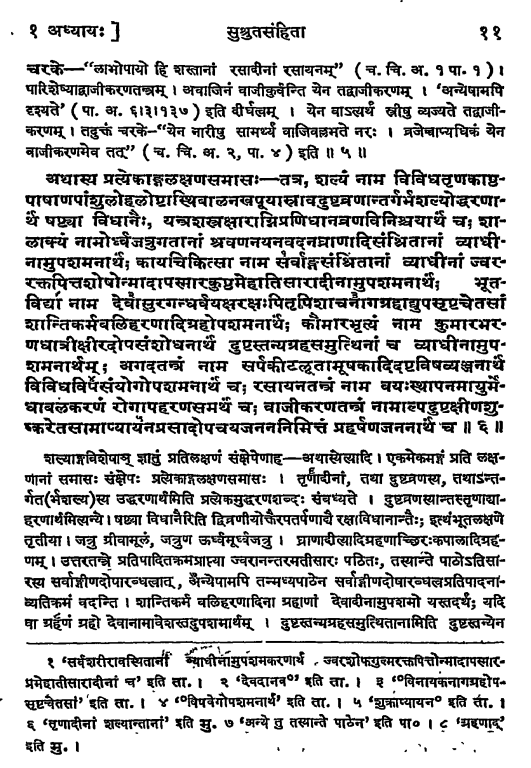
\includegraphics[height=.9\textheight]{media/Bhanumati-page-11}
    \caption{A page of the 1939 \emph{Bhānumatī} edition, showing the variant readings in 
        the 
        footnotes.}
    \label{fig:bhanumati-page-11}
\end{figure}


\subsubsection{The sources for the Bhānumatī}

\begin{enumerate}
    \item A printed edition.  Covered the \emph{Bhānumatī} up to chapter Su.sū.40.
    The siglum was \dev{mu} for \emph{mudrita}.\footnote{\cite{sena-1886}.  
    The
    manuscript on which this edition was based is probably in the library of the
    Calcutta Sanskrit College, and described in \cite[v.\,X.1]{sast-1917}, which
    is not available to me.  See also \cite[IB, 495, n.\,57]{meul-hist} for
    mention of this manuscript.  The reference at \cite[217]{rao-sans} to CSCL
    accession number 97 in Bengali script may be this manuscript.}
    
    \item A manuscript in the India Office Library library provided through the
    Bhandarkar Oriental Research Institute in Pune.\footnote{At this time,
    manuscripts from Britain were routinely lent to scholars in India and vice
    versa.} This manuscript covered the \emph{Bhānumatī} b up to the end of the
    \emph{sūtrasthāna}.  The siglum was \dev{ha} for
    \dev{hastalikhita}.\footnote{\MScite{London BL H. T. Colebrooke 908}
    (\href{panditproject.org/entity/109978/manuscript}{PanditProject \#109978},
    consulted on July 03, 2021).}
\end{enumerate}

\subsubsection{The sources for the Suśrutasaṃhitā}

\begin{enumerate}
    \item A palm leaf manuscript from Hemarājaśarman's personal
    library.\footnote{I.e., \MScite{Kathmandu NAK 5-333}.}  The siglum was
    \dev{tā} for \dev{tāḍapatra}.
    
    \item His own published edition. The siglum was \dev{ḍa} for \dev{ḍalhaṇasaṃmataḥ
        pāṭhaḥ}.\footnote{\cite{vulgate}.  It is noteworthy that Ācārya refers to
    his 1938 edition as representing “the Ḍalhaṇa recension.”}
    
    \item Hārāṇacandra Cakravarti's published edition with his own
    commentary.\footcite{bhat-1917} The siglum was \dev{hā}.
\end{enumerate}
%
\subsection{Evaluation}

The main innovation of this publication was to present the only surviving part of
the commentary on the \SS\ by the great eleventh-century medical scholar
Cakrapāṇidatta, namely the \emph{Bhānumatī}.\footcite[IA, 374--375 and IB,
495--496]{meul-hist} A secondary purpose was to present the text of the
\emph{sūtrasthāna} as read in \MScite{Kathmandu NAK 5-333}, that had recently been
brought to the editors' attention. In their judgement, the Kathmandu manuscript
presented a text that was closer to what Cakrapāṇidatta had before him than the
text according to Ḍalhaṇa.   This was the first \SS\ edition in which Ācārya used
sigla to identify the sources from which variant readings were reported, so while
it has limitations, it for the first time enables us to get some idea of origins
of the text (see Figure~\ref{fig:bhanumati-page-11}).

Ācārya noted in his introduction that the manuscripts containing the Ḍalhaṇa's
commentary all came together with the root-text of the \SS, and thus the main \SS\
text reflected the readings chosen by Ḍalhaṇa.  But the manuscripts of the
\emph{Bhānumatī} contained the commentary alone, without the root-text, and had
many explanations based on different readings of the root-text than those of
Ḍalhaṇa.  In many of these cases it was hard to know what the text that
Cakrapāṇidatta had before him. But Ācārya noted that Cakrapāṇidatta had a text
before him that had much in common with the text of the Nepalese
manuscript.\footnote{\cite[3--4]{acar-1939}.  See discussion by
\citet[7]{kleb-2021a}.}  

There is compelling evidence that Cakrapāṇidattas's \emph{Bhānumatī} commentary
once covered the whole text of the \SS.\footcite[IA, 375]{meul-hist}  The loss of
the rest of the work ranks amongst the greatest disasters in Āyurvedic
literature.  Remarkably, the whole \emph{Bhānumatī} may still have existed in the
early twentieth century. In 1903, Palmyr Cordier reported being privately informed
of a complete copy of the work in a personal manuscript collection in
Benares.\footcite[332]{cord-1903}

        \section{Features of the manuscript transmission}

\subsection{Palaeographical features}
\begin{itemize}
    \item śrita for śṛta.
    \item ś and s in KL 699.
\end{itemize}

\subsubsection{Chart of characters}

[[[Put a chart from QuickPalaeographer here.]]]

\newpage


        % !TeX root = incremental_SS_Translation.tex

\chapter{Sūtrasthāna 1: The Origin of Medical Knowledge}

\section{Literature}

Meulenbeld offered an annotated overview of this chapter and a bibliography
of earlier scholarship to 2002.\fvolcite{IA}[203--204]{meul-hist} 

\section{Translation}

\begin{translation}
    
    \item[1] Now I shall narrate the chapter on the origin of this
    knowledge.\footnote{Ḍalhaṇa understood the word "\se{veda}{knowledge}" as
    specifically "medical knowledge." He said that the word "longevity"
    (\emph{āyur}) \ssaneng{āyur}{life, longevity} had been elided.
    %    
    %    Notes Dec 8:
    %    Dominik: N's ādhyāyaṃ corruption of H's nāmādhyāyaṃ: possible evidence that N was 
    %created 
    %after H
    %    Check: Ācārya 1931 footnote on vedotpattim
    %    Commentary Ḍalhaṇa (c. 1200 CE) notes āyur dropped from veda in vedotpattim
    %    
    %    
    After this opening statement, later manuscripts and commentaries include
    the attribution, "as the venerable Dhanvantari stated."  The absence of this
    statement in the early Nepalese manuscripts is highly significant because it 
    removes
    the outer narrative frame of the \SS\
    \parencites[148]{wuja-2013}[\S\,3.1.2]{kleb-2021b}{rai-2019}{birc-2021}.  On 
    the 
    figure of Dhanvatari in 
    medical literature, see \cite[IA 358--361]{meul-hist}.} %     <!-- Notes Dec 8:
    %    Dom: note the omission of Dhanvantari, which is in the edition.
    %    On Dhanvantari, see Meulenbeld HIM, authorities associated with Suśruta. He's
    % an authority on
    %surgery or toxicology-->
    
    \item[2] Now, as is well-known, Aupadhenava, Vaitaraṇa, Aurabhra, Puṣkalāvata,
    Karavīra, Gopurarakṣita, \diff{Bhoja}, Suśruta and others addressed Lord 
    Divodāsa,
    king of Kāśi, the best of the immortals, who was in his ashram surrounded by
    an entourage of sages.\footnote{On these persons, see \cite[IA
    361--363, 369\,ff.]{meul-hist}. The authority Bhoja does not appear in the list as
    published in the vulgate edition \citep[1]{susr-trikamji2}, and was not
    included in \cite{meul-hist} amongst “authorities mentioned in the \SS.” 
    \citeauthor{meul-hist} gathered textual evidence about Bhoja at \cite[IA
    690--691]{meul-hist}. \citet{kleb-2021a} has discussed these authors in the
    context of an anonymous commentary on the \SS\ that cites them.}
    
    \nocite{emen-1969}
    
    %    Notes Dec 8:
    %    Dom: Check these names in Meulenbeld 
    %    Bhoja is an early lost authority on medicine. Not the same person as King Bhoja, 
    %commentator 
    %on the Yogasūtras.
    %    Ḍalhaṇa's comm. mentions Bhoja as also included in prabhṛtayaḥ: so the version of 
    %the text he 
    %was using did not mention Bhoja, but he was aware of him: His provenance makes it 
    %possible that 
    %he knew the Nepalese version of the SŚ
    
    \item[3]
    %O Lord, after seeing people who are assailed by the impingements of various pains 
    %caused by 
    %physical, mental and accidental diseases, who have the support of friends [but] 
    %feeling as if they 
    %were alone, and acting frantically, shouting out, we have been distressed. 
    
    “O Lord, distress arose in our minds after witnessing people thrashing about with
    cries, assailed by different kinds of \se{vedanābhighāta}{pain and injury}, 
    feeling helpless in spite 
    of having friends, because of diseases arising from the body, the mind and
    external sources.
    
    
    
    %    Notes Dec 8:
    %    āgantu - caused by something from outside the body
    %    abhighāta - threats, impingements 
    %    vedanābhighāta - tatpuruṣa 
    %    anātha - among a list of people who shouldn't be treated.
    %    Ḍalhaṇa- sanātha: samitra someone with a friend -->
    
    \let\uncertain\texttt
    
    \item[4]    
    “To quell the illnesses of those who seek happiness and for our own purpose of
    prolonging life, we desire \se{āyurveda}{the science of life} that is being
    taught.  Welfare\ssaneng{śreyas}{welfare}, both in this world and in
    the next, depends upon it. Therefore, we have come to the Lord in pupillage." %
    % reading bhagavan (voc.) and tam (it, ayurveda, masc. acc.)
    
    % we think upasannāḥ smaḥ is probably wrong, but we can't see how to improve it.
    % upapannā sma ?
    
    \item[5] The Lord said to them:
    
    “Welcome to you!  My children, all of you are beyond reproach and worthy 
    to be taught.
    
    
    \item[6] 
    %    "As is well-known in this world, before creating people, Brahmā composed 
    %    what is called Āyurveda.\footnote{The relative pronoun \emph{yad}, that has 
    %no  
    %    correlative \citep[\P 461]{spei-1886}, is omitted.} 
    %    It is taught as part of the \emph{Atharvaveda}, in hundreds of 
    %    thousands of verses and a thousand chapters and, after observing the short 
    %    lifespan and low intelligence of people, made it again in eight parts. 
    %    %infer tat as the object of kṛtavān
    %    
    
    “As is well known, Ayurveda is the name of what is said to be the subsidiary
    part of the Atharvaveda.   Before creating people, Svayambhū composed it in
    hundreds of thousands of verses and a thousand chapters and, after observing the
    short lifespan and low intelligence of people, he presented it again in eight
    parts.\footnote{Svayambhū is another name for Brahmā, the creator.}
    
    \item[7] “Surgery, treatment of body parts above the clavicle, general medicine, 
    knowledge of spirits, care of children, and the disciplines of antidotes, rejuvenation 
    and aphrodisiacs.
    % why do some of the auxiliaries end in tantra? Dom: Some were disciplines that had a 
    %separate life outside āyurveda. The others were more particular to vaidyas.
    
    \item[8] “Now,  a collection of the characteristics of each component of 
    Āyurveda.
    
    \item[9] “Among them, [the component] called surgery has the goal of 
    extracting 
    various grasses, wood, stone, dust, iron (?), soil, bone, hair, nails, discharge of 
    pus, malignant wounds and foreign bodies inside the womb, and of determining 
    the application of surgical instruments, knives, caustics and fire by means of 
    sixty definitions.
    %Ḍalhaṇa seems to read duṣṭavraṇāntar, and glosses antar as madhyāt. He then reads 
    %garbhaśalya (HIM - foetuses stuck in the womb). Ḍalhaṇa is aware of the reading ṣaṣṭyā 
    %vidhānaiḥ (following uddhraṇārtha), and says some explain it as apatarpaṇādyai 
    %rakṣāvidhānāntair dvivraṇīyoktair ity arthaḥ. However, mss. 699 and 533 read abhi° not 
    %vi°
    
    \item[10] “[The component] named the doctrine of treating body parts above 
    the clavicles has the aim of curing diseases situated above clavicles that is,  
    diseases located in ears, eyes, mouth, nose and so on.
    
    \item[11] “[The component] called general medicine has the goal of curing 
    illnesses established in the whole body and [diseases] such as fever, tumour, 
    swelling, hemorrhagic disorders, insanity, epilepsy, urinary diseases, diarrhoea 
    and the like.
    
    \item[12] “[The component] called knowledge of spirits is for appeasing
    demons by pacification rites and making food offerings for those whose
    minds have been possessed by gods, their enemies,\footnote{Dānavas.  The
    insertion marks (\emph{kākapada}s) below the text at this point appears to
    be by the original scribe.} Gandharvas, Yakṣas, demons, deceased
    ancestors, Piśācas, Vināyakas, \footnote{The vulgate doesn't have
    \emph{vināyaka}s but does add \emph{asura}s, probably under the influence
    of Ḍalhaṇa.  Cite Paul Courtright, Ganesha book.} Nāgas and evil spirits
    that possess children. % Notes: vināyaka is omitted from the vulgate. In
    % Mahābhārata, etc. It refers to
    %a class of demons.-->
    
    
    \item[13] “[The component] called care of children is for bearing children and 
    purifying defects in a wet-nurse's milk, and curing diseases that have arisen 
    from bad breast milk and demons.
    
    \item[14] “[The component] called the discipline of toxicology is for
    [knowing] the signs of poison from snake and insect bites and for
    neutralising various combinations of poisons.\footnote{The scribal
    insertion marks (crosses) above the line at this point in MS K appear to
    be in a later hand and their referent is lost in the damaged part of the
    folio.  Although MSS \MScite{Kathmandu NAK 1-1079} and \MScite{Kathmandu 
    NAK 5-333} include \se{lūtā}{spiders} and
    \se{sarīsṛpa}{creepy-crawlies} in the list, it does seem that MS K had
    a shorter list, and the vulgate edition adds \se{mūṣika}{rodents}.}
    
    \item[15] “[The component] called the discipline of rejuvenation is 
    maintaining 
    youth, bringing about a long life and mental vigour and for curing diseases.
    
    % Got to here 2021-01-13
    
    \item[16] “[The component] called the discipline of aphrodisiacs brings about 
    the 
    increase, purity, accumulation and  production of semen for those whose semen 
    is minimal, bad, depleted, and dry [respectively] and for inducing an erection.
    
    \item[17] “Thus, this Āyurveda is taught with eight components."
    
    "Among these [components], tell us which is for whom."
    
    \item[18] They said, "After you have conveyed the knowledge of surgery, 
    teach 
    us everything."
    
    \item[19] He said, "so be it."
    
    \item[20] They then said, "Having considered the view of all of us, when we 
    are 
    unanimous, Suśruta will question you. We too will learn what is being taught to 
    him."
    
    \item[21] He said, "so be it.
    
    \item[22] “Now, as is well-known, the aim of Āyurveda is eliminating the 
    disease of one who have been assailed by disease and protecting the healthy;  
    āyurveda is [that knowledge] in which they find a long life, or that by which 
    long life is known. Learn its best component (i.e., surgery), which is being 
    taught in accordance with tradition, perception, inference and analogy.
    
    \item[23] "For this component is first, the most important, because it is 
    referred to first; it cures wounds and joins together the most important thing, 
    Yajña's head. For, just as it has been said of old, 'the head that had been cut off 
    by Rudra was joined again by the two Aśvins.'
    
    \item[24] "And also, of the eight disciplines of Āyurveda, [surgery] alone is 
    the best because of the quick action of its \se{kriyā}{procedures}, its 
    application of blunt 
    instruments, knives, caustics and fire, and it is common to all disciplines.
    
    \item[25] "Therefore, [surgery] is eternal, meritorious, leads to heaven, 
    brings renown, bestows a long life, and affords a livelihood.
    
    \item[26] "Brahmā said this, 'Prajāpati learned it. From him, the Aśvins. From 
    the Aśvins, 
    Indra. From Indra, I. In this world, I will transmit to those who desire it for the benefit of 
    people.' 
    
    [There a verse about this.].\footnote{This is an expansion 
    of the scribe's abbreviation \emph{bha} for \emph{bhavati cātra ślokaḥ} 
    “There is a verse about this” (sometimes plural).\label{bha}}
    
    \item[27]           
    \begin{sloka}
        For, I (i.e., Brahmā) am Dhanvantari, the first god, the remover of old age, 
        pain and 
        death of mortals.\\ Having understood surgery, the best of the great 
        knowledge 
        systems, I arrived on earth again to teach it here.
    \end{sloka}    
    
    % draft tr.
    
    \item[28] In this context, as far as this discipline is concerned, a 
    \se{puruṣa}{human being} is called an amalgam of the five elements 
    and the embodied soul.  This is where \se{kriyā}{procedures} apply. This 
    is the locus. 
    
    Why?
    
    Because of the duality of the world, the world is twofold: the stationary
    and the moving. Its \se{ātmaka}{nature} is twofold, depending on the
    preponderance of Agni and Soma.\footcite[See][]{wuja-2004}  Alternatively,
    it can be considered as being fivefold.  The multitude of beings in it are
    fourfold: they are termed “sweat-born, stone-born, caul-born and
    egg-born”.\footnote{This fourfold classification of beings is paralleled
    with closely-related vocabulary in  \emph{Bhelasaṃhitā} 4.4.4	
    \parencites[206]{kris-2000}[81]{mook-1921}.}  Where they are concerned, the
    human being is the main thing; others are his support.  Therefore, the
    \se{puruṣa}{human being} is the locus.
    
    \item[29]  Diseases are said to be the conjunction of the person and 
    \se{duḥkha}{suffering}.
    There are four of them: invasive, bodily, mental and inherent.  The invasive ones 
    are caused by an injury.  The bodily ones are based on food, caused by 
    \se{vaiṣamya}{irregularities} in wind, bile, phlegm and blood.\footnote{Note 
    that four humoral substances are assumed here.} 
    
    The \se{mānasa}{mental} ones, caused by 
    \se{icchā}{desire} and 
    \se{dveṣa}{hatred}, 
    include:  
    \se{krodha}{anger}, 
    \se{āśoka}{grief}, 
    \se{dainya}{misery}, 
    \se{harṣa}{overexcitement}, 
    \se{kāma}{lust}, 
    \se{viṣāda}{depression},
    \se{īrṣyā}{envy},
    \se{asūyā}{jealousy},
    \se{mātsarya}{malice}, 
    and
    \se{lobha}{greed}.
    
    The \se{svābhāvika}{inherent} ones are hunger, thirst, old age, death, 
    sleep and  those of the \se{prakṛti}{temperament}.
    
    These too are \se{adhiṣṭhāna}{located} in the mind and body.
    
    \se{lekhana}{Scarification},
    \se{bṛṃhaṇa}{nourishment},
    \se{saṃśodhana}{purification},
    \se{saṃśamana}{pacification},
    \se{āhāra}{diet} and
    \se{ācāra}{regimen}, 
    properly employed, bring about their cure.
    
    
    \item [30] Furthermore, food is the  \se{mūla}{root} of living beings as well
    as of \se{bala}{strength}, \se{varṇa}{complexion} and 
    \se{ojas}{vital
        energy}. It \se{āyatta}{depends on} the six \se{rasa}{flavours}.
    Flavours, furthermore, have substances as their \se{āśrayin}{substrate}.  And
    substances are \se{oṣadhī-}{remedies}.\footnote{Pāṇini 6.3.132 provides that
    the final vowel of the noun \emph{oṣadhi} may be lengthened
    (\emph{$\rightarrow$oṣadhī}) under certain conditions.  These conditions require
    that the word be used in a Vedic mantra and not in the nominative.  Neither
    condition is met in this passage, yet the author uses the form \emph{oṣadhī}. 
    This form is in fact not uncommon in medical literature as well as in epics,
    purāṇas, smṛtis, and other parts of Sanskrit literature.} There are 
    two types:
    \se{sthāvara}{stationary} and \se{jaṅgama}{moving}.
    
    
    
    \item [31]  Of these, there are four types of stationary ones:
    \se{vanaspati}{fruit trees}, \se{vṛkṣa}{flowering trees},
    \se{oṣadhi}{herbs} and \se{vīrudh}{shrubs}.\footnote{Ca.sū.1.71--72 
    also
    describes these four types of medicinal plant in similar terms but with slightly
    differing names: \emph{oṣadhi} is a plant that ends after fruiting, \emph{vīrudh}
    is a plant that branches out, \emph{vanaspati} is a tree with fruit, and
    \emph{vānaspatya} is a tree with fruit and flowers.}
    Amongst these, the “fruit trees” have fruit but no flowers.\footnote{The MSS agree 
    in reading \emph{phalavantyaḥ} “having flowers” which is grammatically 
    non-standard. This form is also found in the  \emph{Viṣṇudharmottarapurāṇa} 
    (1.92.27, \cite[1.92.27][56r]{sarm-1912}).}  The “flowering trees” 
    have flowers and fruit.  The “herbs” die when the fruit is ripe. “Shrubs” put out 
    shoots.
    
    % \citep{ober-2003} didn't have anything on phalavantyo that I could find quickly.
    
    
    \item[32]  As is well known, moving remedies are also of four types: those
    \se{jarāyuja}{born in in a caul}, those \se{aṇḍaja}{born from eggs},
    those \se{svedaja}{born of sweat}, and \se{udbhid}{shoots}. Amongst
    these, those born in a caul include \se{paśu}{animals}, humans, and
    \se{vyāla}{wild animals}.  Birds, \se{sarīsṛpa}{creepy-crawlies} and
    snakes are “born of eggs.” \se{kṛmi}{Worms}, \se{kunta}{small insects}
    and \se{pipīlika}{ants} and others are born of sweat.\footnote{The word
    \emph{kunta}, though marked as “lexical” in most dictionaries, is in fact found
    in literature, commonly as a compound with \emph{pipīlika}; the compound
    sometimes seems to be understood a type of ant (\emph{tatpuruṣa} compound)
    rather than as a pair of insects (\emph{dvandva} compound).}  Shoots include
    \se{indragopa}{red velvet mites} and \se{maṇḍūka}{frogs}.\footnote{On
    \emph{indragopa}, see \cite{lien-1978}.}|
    
    \item[33] In this context, among the stationary remedies, 
    \se{tvak}{skin}, 
    \se{patra}{leaves}, 
    \se{puṣpa}{flowers}, 
    \se{phala}{fruits},
    \se{mūla}{roots},
    \se{kanda}{bulbs},
    \se{kṣīra}{sap},
    \se{niryāsa}{resin},
    \se{sāra}{essence},
    \se{sneha}{oil}, 
    and
    \se{svarasa}{juice extract}\footnote{On \se{svarasa}{juice extract} see
    CS 1.1.73, 1.4.7; Ḍalhaṇa on \Su{4.10.12}{450}.} 
    are useful; among the moving remedies 
    \se{carman}{pelt}, hair, nails, and 
    \se{rudhira}{blood} and so forth. 
    
    \item[34] And \se{pārthiva}{earth products} include gold and 
    silver.\footnote{The flow of concepts in the treatise seems to be interrupted here.}
    
    \item[35] The \se{kālakṛta}{items created by time} are \se{samplava}{clusters} 
    as far as wind and \se{nivāta}{no wind}, heat and shade, darkness and light
    and the cold, hot and \se{varṣā}{rainy seasons} are concerned. 
    The divisions of time are the
    \se{nimeṣa}{blink of the eye}, a
    \se{kāṣṭhā}{trice}, 
    \se{kalā}{minutes}, 
    \se{muhūrta}{three-quarters of an hour}, a
    \se{ahorātra}{day and night}, a
    \se{pakṣa}{fortnight}, a
    \se{māsa}{month}, a
    \se{ṛtu}{season}, a
    \se{ayana}{half-year}, a
    \se{saṃvatsara}{year},
    and
    \se{yuga}{yuga}.\footnote{These units are presented at 
    \Su{1.6.5}{24} and discussed by \citet[\S\,59]{haya-2017}.}
    
    
    \item[36]  These naturally cause 
    \se{sañcaya}{accumulation}, 
    \se{prakopa}{irritation}, 
    \se{upaśama}{pacification} 
    and 
    \se{pratīkāra}{alleviation} of the \se{doṣa}{humours}. And they have
    \se{prayojanavat}{practical purposes}.
    
    \medskip[There are verses about this:]\footnote{See footnote \ref{bha}.}
    
    \item[37] 
    \begin{sloka}
        This fourfold category is taught by physicians as a cause for the agitation and 
        quelling of bodily diseases.%
        %
        \footnote{On the topic of the “group of four,” the commentator Ḍalhaṇa
        considers them to be “food, behaviour, earthen products and items created by
        time.”  He refers to the author of the lost commentary entitled \emph{Pañjikā},
        and to Jejjaṭa \citep[IA, 372--3, 192]{meul-hist}.  In his view, these early
        commentators  do not agree that the \se{caturvarga}{fourfold grouping} refers
        to the quartet of \se{sthāvara}{stationary}, \se{jaṅgama}{moving},
        \se{pārthiva}{earthen products} and \se{kālakṛta}{items created by 
        time} \citep[9a]{vulgate}.}
    \end{sloka}
    
    \item[38] \begin{sloka}
        There are two kinds of invasive diseases. Some certainly\footnote{The
        text uses an archaic interjection here, \emph{ha}.} 
        affect (\emph{ni$\surd$ pat}) \index{nipat@ni$\surd$ pat}
        the
        mind, others the body. Their \se{kriyā}{treatment} is of two kinds too.
    \end{sloka}
    
    \item[39]\begin{sloka}
        For those that affect the body there is \se{śārīravad}{physical} 
        therapy, whereas for those that affect the mind there is the 
        \se{varga}{collection} of desirable sensory experiences like sound that 
        bring \se{sukha }{comfort}.
        
    \end{sloka}
    %Those that affect the body have therapy that is  
    %\se{śārīravat}{physical}, whereas for those of the mind it is 
    
    \item [40] 
    
    \se{evam}{Along these lines}, this brief explanation of the 
    \se{catuṣtaya}{four factors}
    is given: \begin{itemize}
        \item    
        \se{puruṣa}{human being},
        \item
        \se{vyadhi}{disease},
        \item
        \se{oṣadhi}{remedies},
        \item
        \se{kriyākāla}{the time for therapies}.
    \end{itemize}
    In this context, 
    \begin{itemize}
        \item from the mention of the word “human,” the collection of 
        substances that arise from it, such as the elements, and the 
        \se{vikalpa}{particulars} of its major 
        and minor \se{aṅga}{parts} such as 
        \se{tvak}{skin}, 
        \se{māṃsa}{flesh}, 
        \se{sirā}{ducts}, 
        \se{snāyu}{sinews}, 
        \se{asthi}{bones} and 
        \se{sandhi}{joints}
        are meant.
        \item
        From the mention of “diseases,” all diseases 
        caused by
        wind, bile, phlegm,
        \se{sannipāta}{congested humours},
        \se{āgantu}{external factors} and 
        \se{svabhāva}{inherent factors} are \se{vyākhyāta}{intended}.
        \item
        From the mention of “remedies,”
        there is the teaching of 
        substances,
        tastes, 
        potencies,
        post-digestive tastes.
        \item
        From the mention of 
        “\se{kriyā}{procedures},”
        \se{karman}{therapies} such as oiling
        and 
        \se{chedya}{excision} are taught.
        \item
        From the mention of the word “time,” every single teaching about the times for
        procedures is meant. 
        
    \end{itemize}
    \medskip[There is a verse about this:]\footnote{See footnote \ref{bha}.}
    
    \item[41]
    
    \begin{sloka}
        This seed of medicine has been declared in brief.  Its explanation will be given in one 
        hundred and twenty chapters.\footnote{This is the number of chapters in the first 
        five sections of the work, namely the  \emph{Sūtra-, Nidāna-, Śārīra-, Cikitsā-} 
        and \emph{Kalpa-sthāna}s. These have 46, 16, 10, 40 and 8 chapters respectively.  The 
        \emph{Uttaratantra} has 66 chapters.}
\end{sloka}

%[There are verses on this:]\q{is this bha
%really in the MSS?}

\item [42] There are one hundred and twenty chapters in five
\se{adhyāya}{sections}.\footnote{On \emph{viṃśa} in the sense of “greater by 20”
see P.5.2.46 \emph{śadantaviṃśateś ca}.}  In that regard, having divided them,
according to their subject matter, into the Ślokasthāna, the Nidāna, the Śārīra,
the Cikitsita and the Kalpa, we shall mention this in the
Uttaratantra.\footnote{The end of this sentence reads oddly.  The vulgate edition
adds an object: “[we shall mention] the remaining topics [in the Uttara]” which
smooths out the difficulty, but this is supported in none of the Nepalese MSS.  At
the start of the Uttaratantra \citep[1.3--4ab]{vulgate} there is indeed a
statement that picks up the point about there being 120 chapters.}

\medskip

[There is a verse about this:]\footnote{See footnote \ref{bha}.}

\item[43]    
\begin{sloka}
    Someone who reads this eternal proclamation of the King of
    Kāśī, that was declared by Svayambhu, will have good karma on earth, will
    be respected by kings and upon death will achieve the world of Śakra.
\end{sloka}

\end{translation}    




             \section{Sūtrasthāna, adhyāya 2}


\subsection{Literature}
\cites[IA, 204]{meul-hist}{prei-2007}[82--83, \emph{et passim}]{wujad-2012}. 

\begin{translation}    
    \item [1] 
    
\end{translation}



% % % % % % % % % % % % % % % % % % % % % % % SS 1.28

        % !TeX root = incremental_SS_Translation.tex
%INTRODUCTION
%A. Preliminaries
%1. Aim of the Article
%2. Importance of 1.16 in the History of Āyurveda 
%B. Text
%1. The Nepalese Version
%2. Vulgate
%3. Differences between the Two (as exemplified by 1.16)
%C. Edition 
%1. Manuscripts
%2. Editorial Principles
%EDITION OF 1.16 

\section{Sūtrasthāna, adhyāya 16}

\begin{translation}    
    
    \item [1] Now we shall expound the method for piercing the ear.\footnote{The 
    topic of  \se{kaṛnavyadha}{piercing the ear} is not discussed in the 
    \emph{Carakasaṃhitā} (\cite[IB, 326, n.\,175]{meul-hist}), but it is mentioned 
    in some texts that followed the \emph{Suśrutasaṃhitā}, such as the 
    \emph{Kaśāpyasaṃhitā} (\cite[IIA, 30]{meul-hist}). Also, the instrument for 
    piercing the ear is described in the \emph{Aṣṭāṅgahṛdayasūtra} 1.26.26 
    \citep[153]{kunt-1902}. In the versions of the text known to Ḍalhaṇa 
    \citep[76]{vulgate} and Cakrapāṇidatta \citep[125]{acar-1939}, the heading of 
    this chapter is \emph{karṇavyadhabandhavidhi} ('the method of piercing and 
    joining the ear'), instead of the Nepalese version's \emph{karṇavyadhavidhi}. 
    The topic of \emph{karṇabandha} is discussed in passages 17--20 of the 
    Nepalese version. However, it appears that only subsequent redactors reflected 
    its importance by including it in chapter headings. The Nepalese version also 
    omits the opening remark on Dhanvantari that appears in subsequent versions. 
    For a discussion of the frame story in the Nepalese version, see 
    \cite{birc-2021}. Ḍalhaṇa \citep[76]{vulgate} and Cakrapāṇidatta 
    \citep[125]{acar-1939} state that only the ears of healthy people should be 
    pierced, and they quote Bhoja to affirm this: 'When piercing the ears of children 
    who are free of disease at these times, their ear flaps and apertures, as well as 
    limbs, increase' (for the Sanskrit, see \cite[76]{vulgate}).}
    \item [2] One may pierce a child's ears for the purpose of preserving and 
    decorating. On renowned days, half days, hours and constellations during the first half of the sixth or seventh lunar month, the boy who has \se{kṛtamaṅgala}{received a benediction}, -- \se{svastivācana}{blessings
        pronounced}\footnote{The
    syntax here is unclear. The expression \emph{svastivācana} may have been
    a gloss inserted into the text at an earlier period to clarify
    \emph{maṅgala}.  But as it stands, it is not syntactically connected to the rest of the sentence. In the versions of 1.16.3 known to Cakrapāṇidatta \citep[126]{acar-1939} and Ḍalhaṇa \citep[76]{vulgate}, the words are united in a compound that reads more naturally.} -- should be placed on the lap of a wet-nurse.\footnote{The versions of 1.16.3 known to Cakrapāṇidatta \citep[126]{acar-1939} and Ḍalhaṇa \citep[76]{vulgate} have the additional compound \emph{kumāradharāṅke} ('on the lap of one who holds the child') after \emph{dhātryaṅke}. The gender of \emph{kumāradhara} is made clear by  Ḍalhaṇa's gloss 'a man who holds the child'. Also, both versions add \emph{bālakrīḍanakaiḥ pralobhya} ('having enticed with children's toys') to indicate that the child should be enticed with toys to stay on the assistant's lap. According to Ḍalhaṇa on \Su{1.16.3}{76}, the toys include replica elephants, horses, bulls and parrots. Ḍalhaṇa further mentions that others read \emph{bhakṣyaviśeṣair vā} ('or by special treats') before \emph{bālakrīḍanakaiḥ}.} Then, while pacifying him and having pulled his ear with the left hand, the physician should use his right hand to pierce the ear straight through at a naturally occurring cleft.\footnote{The versions of 1.16.3 of Cakrapāṇidatta \citep[126]{acar-1939} and Ḍalhaṇa \citep[76]{vulgate} add \emph{ādityakarāvabhāsite} to clarify that this naturally occurring cleft is illuminated by sunshine.} For a boy, do
    the right ear first; for a girl, do the left one. Use a needle on a
    thin ear; an \se{ārā}{awl} on a thick one.\footnote{Ḍalhaṇa on 1.16.3 \citep[76]{vulgate} clarifies that the awl is a shoe-maker's knife for piercing leather.}
    
    \item [3]  If there is excess blood or pain one should know that it was pierced
    in the wrong place. The absence of side-effects is a sign that it has been pierced 
    in the right place.\footnote{At this point, \MScite{Kathmandu KL 699} is missing a folio, so the rest of this chapter
    is constructed on the basis of witnesses \MScite{Kathmandu NAK 5-333} and 
    \MScite{Kathmandu NAK 1-1079}.}
    
    \item [4] In this context, if an ignorant person accidentally pierces a 
    \se{sirā}{duct} there will 
    be fever, burning, \se{śvayathu}{swelling}, pain, \se{granthi}{lumps}, 
    \se{manyāstambhā}{paralysis 
        of the nape of the neck}, 
    \se{apatānaka}{convulsions}, headache or sharp pain in the ear.\footnote{This passage is significantly augmented in 1.16.4 of Cakrapāṇidatta's version \citep[126]{acar-1939} and 1.16.5 of Ḍalhaṇa's \citep[77]{vulgate} to outline the specific problems caused by piercing three ducts called \emph{kālikā}, \emph{marmikā} and \emph{lohitikā}. In fact, the order of the problems mentioned in the Nepalese version has been retained in the other versions and divided between each duct. Cakrapāṇidatta's commentary on 1.16.4 \citep[126]{acar-1939} cites several verses attributed to Bhoja on the problems caused by piercing these three ducts in the ear flap: '\emph{Lohitikā}, \emph{marmikā} and the black ones are the ducts situated in the earflaps.  Listen in due order to the problems that arise when they are pierced. Paralysis of the nape of the neck and convulsions, or sharp pain arise from piercing \emph{lohitikā}. Pain and lumps are thought to arise from piercing \emph{marmikā}. Piercing \emph{kālikā} gives rise to swelling, fever and burning.'}
    
    \item[5]     Having removed the \se{varti}{wick} in the hole because of the aggravation of humours or a culpable piercing,\footnote{In addition to these reasons, 1.16.5 of Cakrapāṇidatta's version \citep[126–127]{acar-1939} and 1.16.6 of Ḍalhaṇa's \citep[77]{vulgate} add \emph{kliṣṭajihmāpraśastasūcīvyadhāt} ('because of piercing with a painful, crooked and unrecommended needle') and \emph{gāḍhataravartitvāt} ('because of a wick that is too thick'). Ḍalhaṇa was aware of the reading in the Nepalese version because he notes in his commentary on 1.16.6 \citep[77]{vulgate} that some read 'because of the accummulation of humours' rather than 'because of piercing with a painful, crooked and unrecommended needle or because of a wick that is too thick.' On the meaning of \emph{samudāya}, see ?? and \cite[1–5]{meul-1992} (ADD PRIMARY REF).} one should smear it with
    a paste of the roots of 
    barley, 
    liquorice, 
    \se{mañjiṣṭhā}{Indian madder}, and the
    \se{gandharvahasta}{castor oil tree},
    thickened with honey and ghee. When it has healed well, one should pierce it again.
    
    \item[6] One should treat the properly-pierced ear by sprinkling it with raw sesame
    oil.   After every three days one should apply a thicker \se{varti}{wick} and
    sprinkle oil right on it.\footnote{The manuscripts support the reading
    \emph{sthūlatarīṃ} that is either a non-standard form or a scribal error.}
    
    \item[7]
    Once the ear is free from humours or side-effects, one should 
    loosen it with a light \se{pravardhanaka}{dilator} in order to enlarge it.\footnote{Cakrapāṇidatta on 1.16.6 \citep[127]{acar-1939} and Ḍalhaṇa on 1.16.8 \citep[77]{vulgate} point out that the dilator can be made of wood, such as that of the \se{apāmarga}{prickly chaff flower}, the \se{nimba}{neem tree} and the \se{kārpāsa}{cotton plant}. Ḍalhaṇa adds that it can also be made of \se{sīsaka}{lead} and should have the shape of the \se{dhattūrapuṣpa}{datura flower}.}
    
    \item[8]
    
    \begin{verse}

A person's ear enlarged in this way can split in two, either as a result of the humours\footnote{Ḍalhaṇa on 1.16.9  \citep[77]{vulgate} notes that the word \emph{doṣa} here can refer to either a humour, such as \se{vāta}{wind}, as we have understood it, or a disease generated from a humour.} or a blow. Listen to me about the \se{sandhāna}{joins} it can have.
        
    \end{verse}
    
        \item[9]
    
Here, there are, in brief, fifteen ways of mending the ear flap.\footnote{The Nepalese version uses the word \emph{sandhāna} to refer to joining a split in an ear flap, which is consistent with the terminology in the verse cited above (8). However, 1.16.10 of Ḍalhaṇa's version \citep[77]{vulgate} uses the term \emph{bandha} here and at the very beginning of the chapter (i.e., 1.16.1) to introduce the topic of repairing the ear.}  They are as follows:
    \se{nemīsandhānakaḥ}{Rim-join}, \se{utpalabhedyaka}{Lotus-splittable}, \se{vallūraka}{Dried Flesh}, \se{āsaṅgima}{Fastening}, \se{gaṇḍakarṇa}{Cheek-ear}, \se{āhārya}{Take away}, \se{nirvedhima}{Ready-Split}, \se{vyāyojima}{Multi-joins}, \se{kapāṭasandhika}{Door-hinge}, \se{ardhakapāṭasandhika}{Half door-hinge}, 
    \se{saṃkṣipta}{Compressed}, \se{hīnakarṇa}{Reduced-ear},
    \se{vallīkarṇa}{Creeper-ear}, \se{yaṣṭīkarṇa}{Stick-ear}, and \se{kākauṣṭha}{Crow's lip}.\footnote{For an artist's impression of these different kinds of joins in the ear flap, see \cite[290]{majn-1975} (reproduced as Figure 3.2 in \cite[154]{wuja-2003}).}
    
    In this context, among these, 
    \begin{description}
        
        \item[\mdseries``Rim-join'' (\emph{nemīsandhānaka}):]
        both flaps are wide, long, and equal.
        
        \item[\mdseries``Lotus-splittable'' (\emph{utpalabhedyaka}):]
        both flaps are round, long, and equal.
        
        \item[\mdseries``Dried flesh'' (\emph{vallūraka}):]
        both flaps are short, round, and equal.
        
        \item[\mdseries``Fastening'' (\emph{āsaṅgima}):]
        one flap is longer on the inside.
        
        \item[\mdseries``Cheek-ear'' (\emph{gaṇḍakarṇa}):]
        one flap is longer on the outside.\footnote{For an artist's impression of this join, see \cite[291]{majn-1975} (reproduced as Figure 3.3 in \cites[155]{wuja-2003}).}
        
        \item[\mdseries``Take-away'' (\emph{āhārya}):]
        the flaps are missing, in fact, on both sides.
        
        \item[\mdseries``Ready-split'' (\emph{nirvedhima}):]
        the flaps are like a \se{pīṭha}{dais}.
        
        \item[\mdseries``Multi-joins'' (\emph{vyāyojima}):]
        one flap is small, the other thick, one flap is equal, the other unequal.
        
        \item[\mdseries``Door-hinge'' (\emph{kapāṭasandhika}):]
        the flap on the inside is long, the other is small.
        
        \item[\mdseries``Half door-hinge'' (\emph{ardhakapāṭasandhika}):]
        the flap on the outside is long, the other is small.
    \end{description}

    `These ten \se{vikalpa}{options} for \se{sandhi}{joins} of the ear should be
    bound.  They can mostly be explained as resembling their names.\footnote{Cakrapāṇidatta on 1.16.9–13 \citep[128–129]{acar-1939} and Ḍalhaṇa on \Su{1.16.10}{77–78} provide examples of how the names of these joins describe their shapes. For example, the \se{nemīsandhānaka}{rim-join} is similar to the join of the \se{cakradhārā}{rim of a wheel}.}  The five from \se{saṃkṣipta}{compressed} on are incurable.\footnote{Ḍalhaṇa on \Su{1.16.10}{77–78} mentions that some do not read the statement that only five are incurable, and they understand the causes of unsuccessful joins given below (i.e., heat, inflammation, suppuration and swelling) as also pertaining to the first ten when they do heal.}  Among these, “compressed” has a dry ear canal and the other flap is small.   “Reduced ear” has 
    flaps that have no base and have wasted flesh on their edges. “Creeper-ear” has 
    flaps that are thin and uneven. “Stick-ear” has \se{granthita}{lumpy} flesh and the 
    flaps are stretched thin and have \se{stabdha}{stiff} \se{sirā}{ducts}.  “Crow-lip” 
    has a flap 
    without flesh with \se{saṃkṣipta}{compressed} tips and little blood. Even when 
    they are bound up, they do not heal because they are hot, inflamed, 
    \se{srāva}{suppurating}, or swollen.\footnote{The version of 1.16.11–13 known to Ḍalhaṇa \citep[78]{vulgate} has four verses (\emph{śloka}) at this point that are not in the Nepalese manuscripts. The additional verses iterate the types of joins required for ear flaps that are missing, elongated, thick, wide, etc. All four verses were probably absent in the version of the \emph{Suśrutasaṃhitā} known to Cakrapāṇidatta. He cites the verses separately in his commentary, the \emph{Bhānumatī} \citep[128–129]{acar-1939}, introducing each one as 'some people read' (\emph{ke cit paṭhanti}). However,  in Trikamajī Ācārya's edition of the \emph{Sūtrasthāna} of the \emph{Bhānumatī}, the root text is largely identical to the one commented on by Ḍalhaṇa (\cite{vulgate}), even in instances like this where Cakrapāṇidatta's commentary indicates that he was reading a different version of the \emph{Suśrutasaṃhitā}.}
    
    \item[10]  
    
    % 15
    A person wishing to perform any of these joins should therefore gather together the
    supplies prepared according to the recommendations of the `Preparatory
    Supplies' chapter.\footnote{\emph{Suśrutasaṃhitā} 1.5 \citep[18–23]{vulgate}.}  And in particular, he should gather
    \se{surāmaṇḍa}{decanted liquor}, milk, water,
    \se{dhānyāmla}{fermented rice-water}, and \se{kapālacūrṇa}{powdered 
        earthenware crockery}.\footnote{The term \emph{kapālacūrṇa} is unusual. Ḍalhaṇa \citep[79]{vulgate} defines it as the powder of fragments of fresh earthen pots and Cakrapāṇidatta \citep[129]{acar-1939} as the powder of earthenware vessels.}  
    
    Next, he should prepare the woman or man, who have had the ends of their hair tied 
    up, have eaten lightly, and are firmly supported by qualified 
    attendants.
    
    Then, he should ready the \se{bandha}{bindings} and carry out the procedure with
    \se{chedya}{cutting}, \se{bhedya}{splitting}, \se{lekhya}{scarification}, or
    \se{vyadhana}{piercing}. Then, he should examine the blood of the ear to know whether it is 
    \se{duṣṭa}{tainted} or not. If it is tainted by wind, the ear should be
    bathed with \se{dhānyāmla}{fermented rice-water} and water; if tainted by choler, 
    then cold water
    and milk should be used; if tainted by phlegm, then \se{surāmaṇḍa}{decanted 
        liquor} and water
    should be used, and then he should scarify it again.
    
    
    Then, arranging the join in the ear so that it is neither proud, depressed, nor
    uneven, one should make the join. Having seen that the bloood has stopped, one should anoint it with honey and ghee,
    bandage each ear with \se{picu}{cotton} and \se{prota}{gauze}, and
    bind it up with a thread, neither too tightly nor too loosely.  Then, the earthenware
    powder should be sprinkled on, and \se{ācārika}{medical advice} given.
    And he should supplement with food as taught in  the `Two Wound'
    chapter.\footnote{\emph{Suśrutasaṃhitā} 4.1 \citep[396–408]{vulgate}.}
    
    \item[11]
    \begin{verse}
        One should avoid rubbing, sleeping during the day, exercise, overeating,
        sex, getting hot by a fire, or the effort of speaking.
    \end{verse}
    
    \item[12]
    
    % 17
    One should not make a join when the blood is too pure, too copious, or too
    thin.\footnote{1.16.17 of Ḍalhaṇa's version \citep[79]{vulgate} reads “impure” for the Nepalese “too pure,” which would
    appear to make better medical sense.  Emending the text to \emph{nāśuddha-} for
    \emph{nātiśuddha-} in the Nepalese recension would yield the same meaning as the
    Ḍalhaṇa's version.} For when the ear is tainted by wind, then it is
    \se{raktabaddha}{obstructed by blood}, unhealed and will peel. When tainted with
    choler, is becomes \se{gāḍha}{pinched}, \se{pāka}{septic} and red.  When tainted
    by phlegm, it will be \se{stabdha}{stiff} and itchy.  It has excessively copious
    \se{srāva}{suppuration} and is \se{puffed up}{śopha}.  It has it has a small
    amount of \se{kṣīṇa}{wasted} flesh and it will not grow.\footnote{In his edition of \emph{Suśrutasaṃhitā}, Ācārya \citep[79 n. 1]{vulgate} includes in parentheses the following treatment for these conditions, which according to a footnote is not found in the palm-leaf manuscript he used: 'One should sprinkle it with raw sesame oil for three days and one should renew the cotton bandage after three days' (\emph{āmatailena trirātraṃ pariṣecayet trirātrāc ca picuṃ parivartayet}).}
    
    \item[13] When the ear is properly healed and there are no complications,  one may
    very gradually start to expand it.  Otherwise, it may be \se{saṃrambha}{inflamed},
    burning, septic or painful.  It may even split open again.
    
    
    \item [14]
    
    
    Now, massage for the healthy ear, in order to enlarge it. 
    
    \newcommand{\animal}[4]{#1 (\emph{#2}\footnote{#3 (#4)})}
    \newcommand{\plant}[4]{#1 (\emph{#2}\footnote{#3 (#4)})}
    \newcommand\skt[2]{#1 (#2)}
    
    One should gather as much as one can the following: a
    \animal{monitor lizard}{godhā}{Varanus bengalensis, Schneider}{Daniel
        1983:58},
    \se{pratuda}{scavenging} and \se{viṣkira}{seed-eating} birds, and
    creatures that live in marshes or water,\footnote{For such classifications,
    see \citet{zimm-1999} and \citet{smit-1994}.} fat, marrow, milk, and sesame oil, and
    white mustard oil.\footnote{1.16.19 of Ḍalhaṇa's version \citep[79]{vulgate} includes \se{sarpis}{ghee}. However, Ḍalhaṇa's remarks on 1.16.19 and Cakrapāṇidatta's on 1.16.18 \citep[130]{acar-1939} indicate that they knew a version of this recipe  (perhaps, similar to the Nepalese) that does not have ghee. Ḍalhaṇa also notes that others simply read four oils, beginning with fat and without milk, whereas Cakrapāṇidatta says some read that it is made with four oils and milk.} %  
% note: think more about the compound structure here.
Then cook the oil with an \se{prativāpa}{admixture} of the following:
    \plant{purple calotropis}{arka}{Calotropis gigantea, (L.) R. Br.}{ADPS 52, AVS
        1.341, NK \#427, Potter 57, ID 306},
    \plant{white calotropis}{alarka}{Calotropis procera, (Ait.) R. Br.}{NK
        \#428, GIMP 46b, ID 306},
    \plant{country mallow}{balā}{Sida cordifolia, L.}{ADPS 71, NK \#2297},
    \plant{`strong Indian mallow'}{atibalā}{Abutilon indicum, (L.) Sweet; Sida
        rhombifolia, L.?}{NK \#11, IGP ,4 1080; NK \#2300},
    %\plant{Indian sarsaparilla}{anantā}{Hemidesmus indicus, (L.) R.
    %  Br. \textnormal{and} Cryptolepis buchanani, Roemer \&
    %  Schultes}{ADPS 434, AVS 3.141, NK \#1210},
    %the \skt{Indian sarsaparillas}{sārive}
    \plant{country sarsaparilla}{anantā}{Hemidesmus indicus, (L.) R. Br.}{ADPS 434,
        AVS 3.141--5, NK \#1210}
    %and
    %\plant{black creeper}{pālindī}{Ichnocarpus frutescens, (L.)
    %    R.Br. \textnormal{or} Cryptolepis buchanani, Roemer \&
    %    Schultes}{AVS 3.141, 3.145, 3.203, NK \#1283, \#1210, ADPS
    %    434}),
    %
    %%\plant{prickly chaff-flower}{apāmārga}{Achyranthes aspera,
    %%    L.}{GJM 524f., IMP 1.39, ADPS 44f., IMP 3.2066f., Dymock 3.135},
    %\plant{Withania}{aśvagandhā}{Withania somnifera (L.) Dunal}{IMP
    %    5.409f., Dymock 2.566f., Chevallier 150.},
    \plant{beggarweed}{vidāri}{Desmodium
        gangeticum (L.) DC}{Dymock 1.428, GJM 602, cf.\ NK
        \#1192; ADPS 382, 414 and IMP 2.319, 4.366 are confusing},
    %\plant{giant potato}{kṣīraśukla  $\rightarrow$ kṣīravidārī}{Ipmoea mauritiana,
    %    Jacq.}{ADPS 510, AVS 3.222, IMP 3.1717ff.},
    liquorice (\emph{madhuka}),
    hornwort (\emph{jalaśūka} $\rightarrow$ \emph{jalanīlikā}\footnote{Ceratophyllum
        demersum, L. (IMP 2371, AVS 2.56, IGP 232). This name is not
    certain. In fact, Ḍalhaṇa on 1.16.19 \citep[79]{vulgate} notes that some people interpret
    it as a poisonous, hairy, air-breathing, underwater creature.}),
    items having the `sweet' savour (\emph{madhuravarga}\footnote{The
    items which exemplify the `sweet' savour \label{kakolyadi}
    (\emph{madhuravarga}) are enumerated at SS.1.42.11.}) and `milk flower'(\emph{payasyā}  $\rightarrow$ \emph{vidārī}\footnote{Pueraria tuberosa (Willd.) 
        DC. (ADPS
        510, IMP 1.792f., AVS 4.391; not Dymock 1.424f. See GJM supplement 444,
        451, IMP 1.187, but IMP 3.1719 = Ipmoea mauritiana, Jacq.). The version of 1.16.19 known to Ḍalhaṇa \citep[79]{vulgate} adds several ingredients to this admixture, including \emph{apāmārga, aśvagandhā, kṣīraśuklā, madhuravarga} and \emph{payasyā}. Also, it has \emph{vidārigandhā} instead of \emph{vidāri}. When commenting on 1.16.19, Ḍalhaṇa \citep[79]{vulgate} notes that some do not read \emph{madhuravarga} and \emph{payasyā}. Therefore, there were probably other versions of this recipe with fewer ingredients, as seen in the Nepalese version.}).
    %
    This should then be deposited in a well-protected spot.
    
    \item[15]% 20
    \begin{verse}
        
        The wise man who has been sweated should rub the \se{mardita}{massaged} ear with 
        it. 
        Then it will be free of complications, and will enlarge properly and be strong.\footnote{For these aims (i.e., healing and enlarging the ear), the text known to Ḍalhaṇa \citep[79]{vulgate} has an additional verse and a half describing an \se{udvartana}{ointment for rubbing the ear} and \se{taila}{sesame oil} cooked with various medicines for massage. Cakrapāṇidatta \citep[131]{acar-1939} does not comment on these verses, nor verse 15 of the Nepalese version, and so the version of the \emph{Suśrutasaṃhitā} known to him may not have included them.}
    \end{verse}
    
    \item[16]
    % 22cd-23
        \begin{verse}
    Ears which do not enlarge even when sweated and oiled, 
    should be scarified
    at the \se{apāṅga}{edge of the hole}, but not outside it.\footnote{Dalhaṇa's version of 
    1.16.23 adds another hemistich that states more explicitly that the scarification should not 
    be done on the outside of hole as it will cause derangement.}  
        \end{verse}
    
    \item[17]
          \begin{verse}
    In this tradition, experts know countless repairs to ears.  So a 
    physician who is \se{suniviṣṭa}{very intent} on working in this way 
    \se{yojayed}{may repair} them.\footnote{After verse 17, the 1938 edition of Ācārya \citep[80]{vulgate} has in parentheses nineteen verses on diseases of the ear lobes, treatments and complications. It is possible that these verses were in some of the witnesses used by Ācārya to construct the text as they occur in other manuscripts, such as  MS Hyderabad Osmania 137-3 (b). However, Cakrapāṇidatta \citep[132]{acar-1939} and Ḍalhaṇa \citep[80]{vulgate} state that some read about the diseases of the ear lobes in this chapter whereas others read about them in the chapter on \se{miśrakacikitsa}{various treatments} (SS 5.25), which does indeed begin with a discussion of the disease \emph{paripoṭa}.  Ḍalhaṇa goes on to say that some believe that these verses were not composed by sages and, therefore, do not read them.}
        \end{verse}
    
    \item[18]
    % 25
           \begin{verse}
    If an ear has grown hair, has a nice hole, a firm join, and is strong and
    even, well-healed, and free from pain, then one can enlarge it slowly.\footnote{The order of verses 17 and 18 are reversed in Ḍalhaṇa's version \citep[80]{vulgate}.}
        \end{verse}
    
    \item[19]
    
    %28, 29.
    Now I shall describe the proper method of repairing a severed nose.
    First, take from the trees a leaf the same size as the man's nose and hang it
    on him. 
    
    \item[20] Next, having cut a \se{vadhra}{slice of flesh}\footnote{The
    version of 1.16.28b known to Ḍalhaṇa \citep[81]{vulgate} reads \se{baddham}{bound, connected} instead of \se{vadhra}{slice of flesh}.
    This is a critical variant from the surgical point of view.  If the slice remains
    connected, it will have a continuing blood supply.  This is one of the effective 
    techniques that so astonished surgeons witnessing a similar operation in Pune in
    the eighteenth century \citep[see][67--70]{wuja-2003}.} with the same
    measurements off the cheek, the end of the nose is then scarified.\footnote{Or 1.16.20 could be mean, 
    `\ldots\ off the cheek, it is fixed to the end of the nose, which has been
    scarified.' Unfortunately, the Sanskrit of the Nepalese version is not unambiguous on the
    important point of whether or not the flap of grafted skin remains connected
    to its original site on the cheek. However, Ḍalhaṇa \citep[81]{vulgate} clarifies the meaning of the vulgate here by stating that one should supply the word 'flesh' when reading 'connected,' thus indicating that he understood the flesh to be connected to the face.} % 
%
Then the \se{apramatta}{diligent} physician, 
    should quickly put it back together so that it is 
    \se{sādhubaddha}{well joined}.
    
    \item[21] 
    % 30.
    Having carefully observed that it has been well sown up,
    two tubes should be fixed in place.\footnote{Ḍalhaṇa on 1.16.21 \citep[81]{vulgate} notes that the two tubes should be made of \se{nala}{reed} or the \se{eraṇḍapatranāla}{stalk of the leaf of castor oil plant}. They should not be made of lead or betel nut because the weight will cause them to slip down.} Then, having lifted them up,\footnote{The 
    Sanskrit term \emph{unnāmayitvā} in 1.16.21 is non-Pāṇinian.}
    the powder of sappanwood (\emph{pattāṅga}\footnote{Caesalpinia sappan, L. (AVS 1.323, IMP 
        2.847f.). For \emph{pattāṅga} there are manuscript variants 
    \emph{pattrāṅga} (MS H) and \emph{pattaṅga}    (N).  Also, MS K (f.\,14r:1) has \emph{pattrāṅga} in a verse in 1.14 (cf. 1.14.36, \cite[66]{vulgate}). In the text known to Ḍalhaṇa (\cite[81]{vulgate}), 1.16.29 has \emph{pataṅga}, and this term is propagated in modern dictionaries.}),
    \plant{liquorice}{yaṣṭīmadhuka}{Glycyrrhiza glabra, L.}{AVS 3.84, NK \#1136},
    and
    Indian barberry\footnote{Berberis aristata, DC (Dymock 1.65, NK
        \#685, GJM 562, IGP 141). Ḍalhaṇa (\cite[81]{vulgate}) understands it as \se{rasāñjana}{Elixir salve}.}\q{añjana}
    should be applied to it.
    
    \item[22] 
    The wound should be covered properly with \skt{cotton}{picu} and should be
    moistened repeatedly with sesame oil.  Ghee should be given to the man to
    drink.  His digestion being complete, he should be oiled and purged in
    accordance with the instructions specific to him.\footnote{The expression 
    \emph{svayathopadeśa} is ungrammatical but supported in all available 
    witnesses.}   
    
    \item[23] %32.
    And once healed and really come together, what is left of that \se{vadhra}{slice of flesh}
    should then be trimmed. If it is  \se{hīna}{reduced}, however, one should make an
    effort to stretch it, and one should make its overgrown flesh smooth.\footnote{Ḍalhaṇa \citep[81]{vulgate} accepts a verse following this, which points out that the procedure for joining the nose is similar to that of joining the lips without fusing the ducts. He notes that earlier teachers did not think this statement on the nose and lips was made by sages, but includes it because it was accepted by Jejjaṭa, Gayadāsa and others. However, Cakrapāṇidatta \citep[133]{acar-1939} does not comment on this additional verse, which suggests that either he did not know of it or was not inclined to accept it.}
    
    
\end{translation}    

        % !TeX root = incremental_SS_Translation.tex
\chapter{Sūtrasthāna 28: Unfavourable Prognosis in Patients 
with Sores}

\section{Literature}

Meulenbeld offered an annotated overview of this chapter and a bibliography
of earlier scholarship to 2002.\fvolcite{IA}[219]{meul-hist} 

\section{Translation}
    
\begin{translation}    
    \item [1] Thus, living creatures and their strength,
\se{varṇa}{complexion} and \se{ojas}{energy} are rooted in food.  That
(food) depends on the six \se{rasa}{flavours}. Thus, the flavours depend
on \se{dravya}{substance}, and substances depend on medicinal herbs. 
There are two kinds of them (herbs):  stationary and 
mobile.\footnote{\Su{1.1.28}{7}, tr.\ \volcite{1}[21]{shar-1999}.}

\end{translation}
        %
        % !TeX root = incremental_SS_Translation.tex
\section{Kalpasthāna, adhyāya 1}

\subsection{Literature}

A brief survey of this chapter's contents and a detailed assessment of the
existing research on it to 2002 was provided by Meulenbeld.\footcite[IA,
289--290]{meul-hist} Translations of this chapter since 2000 have appeared by 
\textcites[131--139]{wuja-2003}[3, 1--15]{shar-susr}.

More recently, a discussion of the fourth chapter of this section in the light of
the Nepalese manuscripts was published by Harimoto.\footcite[101--104]{hari-2011}
After a close comparative reading of lists of poisonous snakes, Harimoto concluded
that, “the Nepalese version is internally consistent while the [vulgate] editions
are not.”  Harimoto showed how the vulgate editions,\footnote{The two editions
\cite{susr-trikamji3} and \cite{bhat-1889}, that Harimoto noted present identical
texts.} had been adjusted textually to smooth over inconsistencies, and gave
insights into these editorial processes.



\subsection{Manuscript notes}

\begin{itemize}
    \item \MScite{Kathmandu NAK 5-333} has foliation letter numerals, for example on f.\,323a,
    that are similar to \MScite{Cambridge Add.\ 
    1693},\footnote{Scan at 
    \href{https://cudl.lib.cam.ac.uk/view/MS-ADD-01693/1}{cudl.lib.cam.ac.uk/view/MS-ADD-01693/1}.}
     dated to 
    1165\,\CE\, noted in Bendall's 
    chart of Nepalese letter-numerals \cite[Lithograph V, after p.\,225]{bend-budd}
\end{itemize}

\newpage

\subsection{Translation}

\begin{translation}
 \item[1--2]  And now I shall explain the procedures for safeguarding food and
%drink, as were declared by the Venerable Dhanvantari.\footnote{MS H adds in the
margin \dev{atha khalu vatsa suśrutaḥ} “Now begins Vatsa Suśruta.”  This phrase
has been copied here by the scribe from the beginning of the \SS\ chapter in the
\emph{sūtrasthāna} on the rules about food and drink (\Su{1.46.3}{214}).  The
scribe presumably felt, not unreasonably, that this section had common subject
matter with the present chapter.  Further, SS 1.46.3 is the only place in the Nepalese 
transmission of the \SS\ that names Dhanvantari and integrates him into the narrative of the 
\SS\ as the teacher of Suśruta. 
  
 The mention of Dhanvantari here is the only other time in the Nepalese
transmission that this authority is cited as the source of Ayurvedic teaching, and the unique 
occurrence of this actual phrase, “as was declared by the Venerable Dhanvantari.”
See the discussion by \citet[28--32]{kleb-2021b}, who concludes that the earliest
recoverable recension of the \SS\ may have had the phrase only at this point and
not elsewhere in the work.}
 
 \item[3]
 

 Divodāsa, the king of the earth, was the foremost supporter of religious
discipline and virtue. With unblemished instruction he taught his students, of
whom Suśruta was the leader.\footnote{This is a quite different statement from
the vulgate \citep[559]{susr-trikamji3} that has Dhanvantari as the teacher, and
calls him the \se{kāśipati}{Lord of Kāśī}.  Ḍalhaṇa followed the vulgate but
explicitly noted the reading before us with small differences: \dev{divodāsaḥ
kṣitipatistapodharmaśrutākaraḥ} “Divodāsa, the king of the earth, was a mine of
traditions about discipline and virtue.”}

\subsection{[Threats to the king]}

\item[4]  

Evil-hearted enemies who have plucked up their courage, may seek to harm the king,
who knows nothing of it.  He may be assailed with poisons by or by his own people
who have been subverted, wishing to pour the poison of their anger into any
vulnerability they can find.\footnote{Verses about the use of Venemous Virgins as a weapon
do not appear in the Nepalese manuscripts. Cf.\ \cite[81\,f., 132]{wuja-2003}}

%A king may be cunningly assailed with poisons by evil-hearted enemies who
%have plucked up their courage, or even by his own people turned traitor,
%wishing to pour the poison of their anger into any chink they can find. Or
%sometimes by women using various concoctions, hoping to make him love
%them.\footnote{On how women of ill-character mix their nail-clippings or
%menstrual blood, etc.\ with the king's food, see
%p.\,\pageref{dusyodara}.} Or again, if a Venomous Virgin is used, a man can
%lose his life instantly.\label{visakanya}
%% \footnote{\label{visakanya}On the `Venomous
%% Virgin', see p.\,\pageref{intro:visakanya}.}



 
    \end{translation}
        % !TeX root = incremental_SS_Translation.tex
\newcommand{\plant}[4]{#1 (\emph{#2})\footnoteA{#3; see #4}}
\let\chemical = \plant
\newcommand{\skt}[2]{#1 (\emph{#2})}
\newcommand{\sskt}[2]{\empty}
%

\chapter{Kalpasthāna 2: Poisonous Plants}

\section{Introduction}

This section begins with several lists of poisonous plants.  The Sanskrit names
for these plants are mostly not standard or familiar from anywhere in Sanskrit or
ethnobotanical literature.  It remains a historical puzzle why these particular
names are so difficult to interpret. However, we are not the first to encounter
these difficulties. In the twelfth century, the learned commentator on the text,
Ḍalhaṇa, remarked,
\begin{quote}
In spite of having made the greatest effort, it has been impossible to identify
these plants. In the Himalayan regions, Kirātas and Śabaras are able to identify
them.\footnote{After \SS, \emph{kalpasthāna} 2.5 \citep[564]{vulgate}. From the
view of Sanskrit authors, Kirāṭas and Śabaras were tribal peoples.  The
eleventh-century author Bhikṣu Govinda, however, cast his treatise as a dialogue 
with a
Kirāṭa king called Madana who was a master of the alchemical art \citep[IIA,
620]{meul-hist}.}
\end{quote}
Ḍalhaṇa also recorded variant readings of these poison names from the manuscripts
that he consulted of the lost commentary of Gayadāsa (fl.\ c.\ \AD\ 1000). The
identities of these poisons have been in doubt for at least a thousand
years.\footnote{See \cite[80--81]{wuja-2003}.}  Identifications have in many cases
    been equally impossible for us today.

One path for exploration in this situation is to attempt to reverse-engineer some 
identifications by considering the known toxic plants of India.\footnote{Valuable 
reference sources on Indian plant toxicology in general include 
\cite[chs.\,10, 11]{pill-2013} and \cite[parts 1.II, 3 and 4]{barc-2008}.}

%\section{Manuscript notes}

\section{Literature}

Meulenbeld offered an annotated overview of this chapter and a bibliography
of earlier scholarship to 2002.\fvolcite{IA}[290--291]{meul-hist} 

\section{Translation}

\begin{translation}
    
    \item[1]
    And now I shall explain \diff{what should be known} about stationary 
    poisons.\footnote{No reference is made to Dhanvantari 
    \citep[see][]{birc-2021}. “Stationary” here is a term contrasted with “moving,” 
    and signifies plants as opposed to animals and insects.}
  
    \item[3]
    \noindent It is said that there are two kinds of poisons,
    \se{sthāvara}{stationary} and \se{jaṅgama}{mobile}. The former
    dwells in ten sites, the latter in sixteen places.
   
    \item[4]
    Traditionally, the ten are: root, leaf, fruit, flower, bark,
    \se{kṣīra}{milky sap}, \se{sāra}{pith}, \se{niryāsa}{resin}, the
    elements (\emph{dhātu})\sse{dhātu}{element}, and the tuber.

    \item[5]
    
    In that context,\label{poisonousplants}
    \begin{itemize}
        \item the eight root-poisons are:\footnote{Some South Asian plants with
    poisonous roots that we would have expected to see in this list include
    \emph{Croton tiglium}, L., \emph{Calotropis} spp., \emph{Citrullus colocynthus} L. 
    Schrad., and \emph{Ricinus
    communis} L.\ \citep{pill-2010}.} 
%    \q{Expected \citep{pill-2010}:\\ Croton
%        tiglium, L. = Naepala, Jayapala, kanakaphala, titteriphala (NL \#720);
%        Calotropis spp.;\\ Citrullus colocynthus (colocynth);\\ Ricinus communis
%        (castor); }
        \begin{enumerate}
        \item  \gls{klītaka},\footnote{Liquorice eaten in excess can be poisonous, but it is 
        unlikely to be the plant intended here.  \citet[124]{gvdb} noted that the 
        poisonous 
        root mentioned in this passage, “remains to be idenitified.”}
       
        \item \gls{aśvamāraka},\footnote{The roots of sweet-scented oleander 
        are highly toxic, as are most parts of the plant \citep{pill-2019}.}
    
        \item \gls{guñjā},\footnote{Jequirity contains a dangerous
        toxin called Abrin in its seeds and to a lesser extent in its leaves,
        but apparently not in its roots or bulb. Abrin is not harmful if eaten,
        but an infusion of the bruised (not boiled) seeds injected or rubbed in
        the eyes can be fatal \citep[\# 6]{NK}.  The dose can be quite small.}
        
        \item \diff{\gls{subhaṅgurā}},\footnote{The plant is
usually called just \emph{bhaṅgurā} without the prefix \emph{su-} “good.”  However, there 
is no reported toxicity associated with \emph{E. prostrata}.  The vulgate reads 
\dev{sugandhā} (\gls{sugandhā}).}
        
       \item \diff{\gls{karaṭā}},\footnote{This poisonous root cannot at present
be securely identified.  Similar-sounding candidates include \emph{karkaṭaka},
\emph{karahāṭa} (emetic nut), and \emph{karaghāṭa}, but since this is a
prose passage, there would be no reason to alter the word to fit a metre.
\citet[255]{moni-sans} cite an unknown lexical source that equates
\emph{karaṭa} (mn.) with safflower (\emph{Carthamus tinctorius}, L.), but
this plant does not have a poisonous root.} 
%
%        \item \plant{luffa}{gargaraka $\rightarrow$ garāgarī?}{Luffa echinata,
%        Roxb.}{NK
%            \#1517},
and ending with 
%
\item \gls{vidyutśikhā},%
%%\plant{leadwort}{vidyutśikhā $\rightarrow$ agni- or
%    rakta-śikhā?}{Plumbago zeylanica (or rosea?), L.}{NK \#1966, 
%    1967}
\footnote{The roots of both rose and white leadwort are very toxic.} 

\item \diff{\gls{anantā} (?)},\footnote{The text reads masculine
    \emph{ananta}, which is not a plant name.  Gayī's commentary on
    \Su{5.2.5}{564} noted a variant reading of feminine \emph{anantā} in
    place of \emph{gargaraka}, earlier in the compound. But the feminine
    \emph{anantā}, \gls{anantā}, is not a poisonous plant.} and

\item \gls{vijayā2},\footnote{\citet[61, n.\,3]{meul-sear} argued that
    our text reads a masculine or neuter noun \emph{vijaya}, which never
    signifies cannabis. However, unlike the vulgate, the unanimous
    readings of the Nepalese manuscripts give feminine \emph{vijayā}. 
    Nevertheless, even the feminine form only started to signify
    \emph{Cannabis sativa} L. after the end of the first millennium
    \citep{meul-sear,wuja-cann,mchu-2021}. The \emph{Sauśrutanighaṇṭu}
    gives a number of synonyms for \emph{vijayā}, almost none of which
    have any poisonous parts \citep[5.77, 10.143]{suve-2000}.  But one of
    them, \emph{viṣāṇī} (also \emph{meṣaśṛṅgī}), is sometimes equated with
    \emph{Dolichandrone falcata (DC.) Seemann} \citep[518]{adps}, a plant
    used as an abortifacient and fish poison \citep[\#862]{NK}.  This
    identification is tenuous.} %
    %        \footnote{Large doses of the root-extract of rauwolfia
    % can be fatal.
    %
    %        In large doses luffa is emetic and a drastic purgative. }
        \end{enumerate}
        \end{itemize}
    
        \item
        the leaf-poisons include:
             \begin{itemize}            
        \item \gls{viṣapatrikā},
        \item \diff{\gls{lambaradā}},
%        \item \plant{`choice tree'}{varadāru}{unknown}{?},
        \item \gls{karambha},
        and
        \item big \gls{karambha};
            \end{itemize}

        \item
        the fruits of items like:
        \gls{guñjā},
        \gls{aruṣkara},
        and
        \gls{viṣavedikā}
        are
\begin{itemize}
         \item \diff{\gls{kumudavatī}},	
         
        \item \diff{\gls{reṇukā}},
        
    \item \diff{\gls{kuruvaka}},

    \item \diff{\gls{veṇuka}},
    
    \item \gls{karambha}
        
    \item \gls{mahākarambha}
    
    \item \diff{\gls{nandanā}},

    \item \diff{\gls{kāka2}},
        
%        \item \plant{ribbed gourd}{karkoṭaka}{Luffa acutangula, (L.) Roxb.? 
%        (Mormodica
%            cochinchinensis, Spreng.? Cf.\ Luffa tuberosa)}{AVS 3.347 (NK \#1640,
%            1643; NK \#1520)}, 
        
%        \item \plant{black cardamom}{hareṇu}{Amomum 
%            subulatum,
%            Roxb.?}{PVS Caraka 2.734, AVS 1.128, NK \#154}, \item \plant{purple
%            calotropis}{khadyotaka $\rightarrow$ arka?}{Calotropis gigantea, (L.) R.
%            Br.}{ADPS 52, AVS 1.341, NK \#427, Potter 63},
%        \item \plant{carmarī}{carmarī}{unknown}{?}, \item 
%        \plant{heliotrope}{ibhagandhā
%            $\rightarrow$ hastiśuṇḍa?}{Heliotropium indicum, L.}{AVS 3.136, NK
%            \#1203},
%        \item \plant{`snake-killer'}{sarpaghāti}{unknown}{?},
%        \item \plant{`gladdener'}{nandana}{unknown}{?}, and
%        \item \plant{`juice-cooker'}{sārapāka}{unknown}{?};\footnote{Bamboo 
%is 
%        not 
%        toxic.
%        Heliotrope flowers are abortifacient in large doses.}

\end{itemize}
    
        \item
        the flower-poisons include those of:
\begin{itemize}
            
        \item \gls{vetra}
        
        \item \plant{wild chinchona}{kādamba}{Anthocephalus cadamba, 
        Miq.}{NK 
        \#204},
        \item \plant{black pepper}{vallīja $\rightarrow$ marica}{Piper
            nigrum, L.?}{NK \#1929; Rā.6.115, Dha.4.85, Dha.2.88},
        \item \plant{thorn apple}{karambha}{Datura metel, L.}{AVS 2.305
            (cf.\ Abhidhāna\-mañjarī), NK \#796\,ff., Potter 292\,f., ADPS 132.},
        and
        \item \plant{big thorn apple}{mahākarambha}{Datura metel, L.?}{AVS 
        2.305
            (cf.\ Abhidhāna\-mañjarī), NK \#796\,ff., Potter 292\,f., ADPS 132.};
            \end{itemize}
        
        \item
        the seven bark, \se{sāra}{pith} and \se{niryāsa}{resin} poisons are:
              \begin{itemize}
            
        \item \plant{`gutboiler'}{antrapācaka}{unknown}{?},
        \item \plant{`blade'}{kartarīya}{unknown}{?},
        \item \plant{wild mustard}{saurīyaka}{Cleome viscosa, L.?
            (cf.\ Rā.4.144)}{AVS 2.116, NK \#615},
        \item \plant{emetic nut}{karaghāṭa $\rightarrow$ karahāṭa? $\rightarrow$
            madana}{Randia dumetorum, Lamk.}{NK \#2091},
        \item \plant{thorn apple}{karambha}{Datura metel, L.}{AVS 2.305
            (cf.\ Abhidhāna\-mañjarī), NK \#796\,ff., Potter 292\,f., ADPS 132.},
        \item \plant{wild asparagus}{nandana $\rightarrow$ 
        bahuputrā?}{Asparagus 
        racemosus,
            Willd.}{ADPS 441, AVS 1.218, NK \#264, IGP 103,
            IMP 4.2499ff., Dymock 482ff.},
        and
        \item \plant{munj grass}{nārācaka}{Saccharum bengalense, Retz.?}{NK
            \#2184};\footnote{The bark of wild asparagus (\emph{Asparagus 
            racemosus}, Willd.)
        is toxic.}
            \end{itemize}
        \item
        the three \se{kṣīra}{milky sap}-poisons are:
              \begin{itemize}
            
        \item \plant{purple calotropis}{kumudaghnī $\rightarrow$ arka?}{Calotropis
            gigantea, (L.) R. Br.}{ADPS 52, AVS 1.341, NK \#427, Potter
            63},\footnote{The name of this poison, \emph{kumuda-ghnī}, means 
            `lotus
        killer'.  In Sanskrit literature, the \emph{kumuda} lotus is associated
        with the moon, since it blossoms by night.  Since the sun causes this lotus
        to close, it is therefore an `enemy' of the lotus.  One of the chief words
        for the sun, \emph{arka}, is also the name of \emph{Calotropis gigantea},
        which indeed has a milky juice which is a violent purgative, poison and
        abortifacient.}
        \item \plant{oleander spurge}{snuhī}{Euphorbia neriifolia, L., 
        \textnormal{or}
            E. antiquorum, L.}{ADPS 448, AVS (2.388), 3.1, NK
            \#988, IGP 457b},
        %   \marginpar{`The milky juice or gum which flows from the branches
        %     [of \emph{E. antiquorum}] is an acrid irritant\ldots. Internally it is a
        %     powerful emetic and a violent purgative, even in very small quantities'.
        %     --- NK \#982}
        and
        \item \plant{`web-milk'}{jālakṣīri}{unknown}{?};
            \end{itemize}
        
        \item
        the two \se{dhātu}{element}-poisons are:
              \begin{itemize}
            
        \item \plant{`foam-stone'}{phenāśma}{unknown}{?}, and
        \item \plant{orpiment}{haritāla}{Arsenii trisulphidum}{NK v.\,2,
            p.\,20\,ff.};\footnote{\citet[38--42]{dutt-1922} conjectured that
        `foam-stone' may be impure white arsenic obtained by roasting orpiment.}
            \end{itemize}
        \item
        the thirteen tuber-poisons are:
        \begin{itemize}
             \item \plant{jequirity}{kālakūṭa}{Abrus
            precatorius, L.? Cf.\ RRS 21.14.}{AVS 1.10, NK \#6, Potter
            168.},\footnote{The much later (perhaps sixteenth century) alchemical
        \emph{Rasa\-ratna\-samuccaya} of pseudo-Vāgbhaṭa (21.14) says that the
        \emph{kāla\-kūṭa} poison, here translated as `jequirity', is similar to
        `\emph{kāka\-cañcu}' or `Crow's Beak', which is indeed a name for the
        plant jequirity or
        \emph{Abrus precatorius}, L., more commonly called \emph{guñjā} (not to
        be confused with \emph{gañjā}). The black seed-pod is described as
        having a `sharp deflexed beak' in botanical descriptions, so the
        Sanskrit name is quite graphic and appropriate. The poisonous scarlet
        seeds of \emph{A. precatorius} can have a distinct black dot or tip,
        which could perhaps be translated `\emph{kāla-kūṭa}', or `Black Tip'.
        
        The \emph{Rāja\-nighaṇṭu\-pariśiṣṭa} (9.35) gives \emph{kālakūṭaka} as a
        synonym for \emph{kāras\-kara}, or \emph{Strychnos nux-vomica}, L., 
        whose
        seeds are notoriously poisonous.}
        \item \plant{wolfsbane}{vatsanābha}{Aconitum napellus, L.}{AVS 1.47,
            NK \#42, Potter 4\,f.},
        \item \plant{Indian mustard}{sarṣapa}{Brassica juncea, Czern. \&
            Coss.}{AVS 1.301, NK \#378},
        \item \plant{leadwort}{pālaka $\rightarrow$  citraka}{Plumbago zeylanica
            (indica? rosea?), L.}{Rā. 6.124, ADPS 119, NK \#1966,
            1967},
        \item \plant{`muddy'}{kardama}{unknown}{?}, the
        \item \plant{`Virāṭa's plant'}{vairāṭaka}{unknown}{?},
        \item \plant{nutgrass}{mustaka}{Cyperus rotundus, L.}{ADPS 316,
            AVS 2.296, NK \#782},
        \item \plant{atis root}{śṛṅgīviṣa}{Aconitum heterophyllum, Wall.
            ex Royle}{AVS 1.42, NK \#39},
        % \item \plant{liquorice}{prapuṇḍarīka $\rightarrow$ 
        %madhuka?}{Glycyrrhiza
        %  glabra, L.}{AVS 3.84, NK \#1136},\footnote{Non-toxic.}
        \item \plant{sacred lotus}{prapuṇḍarīka}{Nelumbo nucifera, Gaertn.}{Dutt 
        110, 
        NK
            \#1698}, \item \plant{radish}{mūlaka}{Raphanus sativus, L.}{NK 
            \#2098},
        \item \plant{`alas, alas'}{hālāhala}{unknown}{Cf. Soḍhalanighantu p.43 
        (sub
            bola) = stomaka = vatsanābha}, \item \plant{`big
            poison'}{mahāviṣa}{unknown}{?}, and \item 
            \plant{galls}{karkaṭa}{Rhus
            succedanea, L.}{NK \#2136}.\footnote{Leadwort root is a powerful poison.
        Nutgrass is tuberous, but non-toxic. Atis has highly toxic tuberous
        roots. Neither sacred lotus nor galls are toxic. The `alas, alas' poison
        (\emph{hālāhala}) is the mythical poison produced from the churning of
        the ocean at the time of creation: it occurs in medical texts such as
        the present one, and commentators identify it with one or other of the
        lethal poisons such as wolfsbane or jequirity.
        \citet[126]{agra-indi} makes the intriguing suggestion
        that the word \emph{hālāhala},
        possibly to be identified with Pāṇini's \emph{hailihila} (P.6.2.38),
        may be of Semitic origin, although his evidence
        seems uncertain (\citet[1506a]{stei-pers} cites Persian \emph{halāhil}
        `deadly (poison)' as a loan from Sanskrit). \cite[iii.585]{mayr-kurz}
        also cites a claim for an Austro-Asiatic origin for the word.}
            \end{itemize}

    Thus, there are fifty-five stationary poisons.
    
    \item[6] There are believed to be four kinds of wolfsbane, two kinds of
\emph{mustaka}, and six kinds of Indian \emph{sarṣapa}.  But the rest are said
to be unique types.
    
    
    
    \subsection{The effects of poisons}
    \item[7--10]
    
People should know that root-poisons cause \se{udveṣṭana}{writhing},
\se{pralāpa}{ranting}, and \se{moha}{delirium}, and  leaf-poisons
cause yawning, writhing, and \se{śvāsa}{wheezing}.
    
 Fruit-poisons cause swelling of the
   scrotum, a burning feeling and writhing.  Flower-poisons will
    cause vomiting, \se{ādhmāna}{distension} and \se{svāpa}{sleep}.  
    
The consumption of poisons from bark, \se{sāra}{pith} and
\se{niryāsa}{resin} will cause foul breath, \se{pāruṣya}{hoarseness},
a headache, and a discharge of \se{kapha}{phlegm}.\footnote{At
    \Su{1.2.6 }{11}, Ḍalhaṇa glossed \se{pāruṣya}{hoarseness} as
    \emph{vāgrūkṣatā}, “a rough, dry voice.”}
    
    % 10
    
The \se{kṣīra}{milky sap}-poisons make one froth at the mouth,  cause
loose stool, and make the tongue feel heavy.\footnote{At
    \Su{6.54.10}{773}, Ḍalhaṇa glossed \se{viḍbheda}{loose stool} as
    \emph{dravapurīṣatā}, “having liquid stool.” }  The
    \se{dhātu}{element}-poisons give one a crushing pain in the chest,
    make one faint and cause a burning feeling on the palate.
    
    % 11
    These poisons
    are classified as ones which are generally speaking lethal after a period of time.
    
    \item[11--17]
    
    \subsubsection{Symptoms of tuber poisoning}
    The tuber-poisons, though, are severe.  I shall talk about them in detail.
    
    %12
    
    With
    \plant{jequirity}{kālakūṭa}{Abrus precatorius, L.?
        Cf.\ RRS 21.14.}{AVS 1.10, NK \#6, Potter 168.}, there is numbness
    and very severe trembling.
    %shivering
%
    With
    \plant{wolfsbane}{vatsanābha}{Aconitum napellus, L.}{AVS 1.47,
        NK \#38, Potter 4\,f.}, there is rigidity of the neck, and the faeces,
    and urine become yellow.
    
    %13
    With \se{sārṣapa}{sārṣapa}%
%With \plant{Indian mustard roots}{sārṣapa}{Brassica juncāea, Czern \&
%    Coss.}{AVS 1.301, NK \#378}
,\footnote{\emph{Sārṣapa} would normally mean
“connected with mustard,” and excessive consumption of mustard oil can be 
harmful. However, the \emph{Sauśrutanighaṇṭu} (156) gives
\emph{rakṣoghnā} as a synonym for \emph{sarṣapā}. This can be
\textit{Semecarpus anacardium}, L.f., which has some poisonous parts.} the
\skt{wind becomes defective}{vātavaiguṇya}, there is \se{ānāha}{constipation},
and \se{granthi}{lumps} start to appear. %
With \plant{leadwort}{pālaka $\rightarrow$  citraka}{Plumbago zeylanica
    (indica? rosea?), L.}{Rā. 6.124, ADPS 119, NK \#1966, 1967}, there is weakness
in the neck, and speech gets jumbled.\footnote{The verse in the Nepalese version 
ends with a plural verb that does not agree with the dual of the sentence subject.}
    
    %14
    With the one called
    \plant{`muddy'}{kardama}{unknown}{?},
    there is a \se{praseka}{discharge}, the faeces pour out, and  the eyes
    turn yellow.
    %
The
    \plant{`Virāṭa's plant'}{vairāṭaka}{unknown}{?}
causes pain in the body and illness in the head.
    %
    Paralysis of one's arms and legs and trembling are said to be caused by
    \se{mustaka}{mustaka}.%
%    \plant{nutgrass}{mustaka}{Cyperus rotundus, L.}{ADPS 316, AVS 2.296,
%        NK \#782} %
\footnote{The substitution 
    in \MScite{NAK 5-333} affecting 15cd is caused by an eye-skip to the word 
    \emph{viṣeṇa} in 2.17.  \emph{Mustaka} commonly refers to Cyperus 
    rotundus, L.; the root is used in āyurveda but is 
    not poisonous.  However other dictionaries list \emph{mustaka} amongst 
    serious poisons, for example \emph{Rājanighaṇṭu} (22 v.\,42) and 
    \emph{Rasaratnasamuccaya} 16, v.\,80.  However, its ancient identity is still 
    doubtful.}
    \item[ 15b]
    With \se{mahāviṣa}{great aconite}\q{-> ativiṣa}
%    \plant{atis root}{śṛṅgīviṣa}{Aconitum heterophyllum, Wall.
%        ex Royle}{AVS 1.42, NK \#39}, 
    one's limbs grow weak, there is a burning
    feeling and swelling of the belly.\footnote{The poisonous root 
    \se{mahāviṣa}{great poison} is not clearly identifiable, although \emph{viṣa} 
    is commonly aconite.  Verse 6 above notes that there are several kinds of 
    aconite.}
    \item[ 16a]
    With \se{puṇḍarīka}{puṇḍarīka},
%    \plant{sacred lotus}{puṇḍarīka}{Nelumbo nucifera, Gaertn.}{Dutt 110,
%        NK \#1698},
    one's eyes go red, and one's belly becomes distended.\footnote{The word 
    \emph{puṇḍarīka} very commonly means sacred lotus, Nelumbo nucifera, 
    Gaertn. The entire plant is edible and cannot be the poison intended here.  
    \citet[252]{gvdb} noted that this poison is unidentified and that it is also 
    listed as a poison in \Cs{ci.23.12}{}.}\q{Look up the ca. reference.}
    \item[ 16b]
    With \se{mūlaka}{mūlaka},
%    \plant{radish}{mūlaka}{Raphanus sativus, L.}{NK \#2098}es,
    one's body is drained of colour and the limbs are paralysed.\footnote{The word 
    \emph{mūlaka} very commonly means the radish, \emph{Raphanus sativus}, 
    L. The root is edible and cannot be the poison intended here.  
    \citet[317]{gvdb} noted that this poison is unidentified.}
    
    %17
    \item[ 17a]
        
    With \se{hālāhala}{aconite}, a man turns a \se{dhyāma}{dark colour}, and
gasps.\footnote{Identification of \emph{hālāhala} is  uncertain. It may simply
be a mythical poison, or its specific identity may have been lost over the
centuries. Late \emph{nighaṇṭu}s identify it as \emph{stomaka} =
\emph{vatsanābha}, i.e., \emph{Aconitum napellus}, L. 
(\emph{Soḍhalanighantu}
p.43). Ḍalhaṇa on \Su{5.2.17}{564} interprets our “gasps” as “the man laughs
and grinds his teeth.”  But this gloss is probably displaced and intended to apply 
to verse 2.18.}

% 5.221 Rājanighaṇṭu

\item[ 17b] With \plant{atis root}{śṛṅgīviṣa}{Aconitum
    heterophyllum, Wall.\ ex Royle}{AVS 1.42, NK \#39}, one gets violent
\se{granthi}{knots} and stabbing pains in the 
heart.\footnote{\citet[407]{gvdb} noted that \emph{vatsanābha} and 
\emph{śṛṅgīviṣa} are two different varieties of poisonous Aconites that are 
difficult to distinguish.}
    
    %18
    \item[ 18a]
    With
    \se{monkey}{markaṭa}, one leaps up, laughs, and 
    bites.\footnote{\citet[299]{gvdb} said of \emph{markaṭa}, “an 
    unidentified vegetable poison.”  Cf.\ \cite[v.36]{suve-2000} for synonyms that 
    lead to the non-toxic jujube tree.}
    
    %{galls}{karkaṭa}{Rhus succedanea, L.}{NK \#2136}
    
    \item[ 18b-19a]
%    Experts said that the thirteen cited highly potent tuber-poisons should be 
%known to have possessed ten features:
%    %()Experts said that one should know that these thirteen cited highly potent 
%%tuber-poisons have ten features:
    %Experts said that these thirteen highly potent tuber-poisons which are 
    %mentioned here consist of ten features.)
    
    Experts have said that one should know that the thirteen highly potent 
    tuber-poisons, which are mentioned here, have ten \se{guṇa}{qualities}.
    
    \item[ 19b--20a]
    
    The ten are:
    \begin{itemize}
        \item    \se{rūkṣa}{dry}, 
        \item hot, 
        \item sharp, 
        \item \se{sūkṣma}{rarified},
        \item     fast-acting, 
        \item \se{vyavāyin}{pervasive}, 
        \item \se{vikāsin}{expansive}, 
        \item \se{viśada}{limpid},
        \item     light, and 
        \item indigestible.    
    \end{itemize}
    %20b
    \item[ 20b]
    Because of dryness, it may cause inflammation of the wind; because of heat
    it inflames the choler and blood. 
    %21
    Because of the sharpness it unhinges the
    mind, and it cuts through the connections with the \skt{sensitive
        points}{marman}.  Because it is rarified it can infiltrate and distort
    the parts of the body.\footnote{We read the active \emph{vikaroti} with 
    Ḍalhaṇa against the 
    transmitted passive \emph{vikriyeta}, since it must be the parts of the body 
    that are distorted, not the poison.}    
    

\item[22]
Because it is fast-acting it kills quickly, and because of its pervasiveness
it affects one's \skt{whole physical constitution}{prakṛti}.\footnote{Ḍalhaṇa
on \Su{5.2.22}{565} explained this as “\se{akhiladehavyāptirūpam}{takes the
form of pervading the whole body}.”}  Because of its expansiveness it enters
into the \se{doṣa}{humour}s, \se{dhātu}{bodily constiuents}s, and even the
impurities\sskt{impurity}{mala}.  Because it is limpid it overflows, and
because it is light it is difficult to treat.  Because it is indigestible it
is hard to eliminate.  Therefore, it causes suffering for a long time.
    
    \item[ 24]
    Any poison that is instantly lethal, whether it be
    stationary, mobile, or artificial, will be known to 
    have all ten of these qualities.
    
    
  
    
    \subsection{Slow-acting poison}
    \item[25cd--26]  
    \begin{verse}
        A poison that is old or destroyed by anti-toxic medicines, or
else dried up by blazing fire, wind, or sunshine, or which has
just spontaneously lost its features,\footnote{Ḍalhaṇa
    specified that this refers to the ten qualities that are
    mentioned above (\Su{5.2.26}{565}).} becomes a
    \skt{slow-acting poison}{dūṣīviṣa}.\footnote{Ḍalhaṇa cited
        this verse at \Su{1.46.83}{222} while explaining
        \emph{dūṣīviṣa} (see p.\.,\pageref{dusivisa}.} Because it has
        lost its potency it is no longer perceived.  Because it is
        surrounded by \se{kapha}{phlegm} it has an aftermath that
        lasts for a very long time.
        
        \item[27] If he is suffering from this, the colour of his stools changes,
he gets a sour, bad taste and is very thirsty. Speaking nonsensically 
and close
to death, wandering about, he may feel faint, giddy, and
aroused.\footnote{Similar symptoms of slow-acting poison are described at
\Su{2.7.11--13}{296} in the context of  \se{duṣyodara}{contamination
dropsy}.  This this may explain why the vulgate inserted reference to this
disease at this point.}
        
        
        
%        Also, he has
%        the symptoms of \skt{contaminated
%            dropsy}{duṣyodara}.
%        \footnote{\label{dusyodara}`Contaminated dropsy'
%        (\emph{duṣyodara} or \emph{dūṣyudara}) is described elsewhere as a
%        condition which arises when women of ill-character mix nail clippings,
%        hair, urine, faeces, or menstrual blood with a man's food, in order to
%        gain power over him (2.7.11--13).}



        \item[28]
        If it lodges in his \se{āmāśaya}{stomach}, he becomes sick because of wind 
        and phlegm; if it lodges in his \se{pakvāśaya}{intestines}, he becomes sick 
        because of  wind and 
        choler.  A man's hair and limbs fall away and he looks like a
        bird whose wings have been chopped off.
        \item[29a--c]
        If it lodges in one of the body tissues such as 
        \se{rasa}{chyle}, it causes the diseases arising
        from the body tissues, that have been said to be wrong.\footnote{The 
        expression \emph{ayathāyathoktān} “stated to be unsuitable” is hard to 
        understand here, but is clearly transmitted in the Nepalese version.}
        and it rapidly becomes inflamed on days that are nasty
        because of cold and wind.
        
        \item[29d--31] Listen to its initial \se{liṅga}{symptoms}: it causes
heaviness due to sleep, yawning, \se{viśleṣa}{disjunction} and
\se{harṣa}{horripilation} and a \se{aṅgamarda}{bruising of the
    limbs}.\footnote{Ḍalhaṇa \Su{5.2.30ab}{565} glossed “disjunction” as the
loss of function of the joints in regard to movement.} Next, it causes
\se{annamada}{intoxication from food} and indigestion, \se{arocaka}{loss
    of appetite}, the condition of having a \se{koṭha}{skin disease} with
\se{maṇḍala}{round blotches},\footnote{The last ailment could perhaps be
ringworm.} % 5.2.31
\diff{\se{kṣaya}{dwindling away} of flesh}, swelling of the feet, hands, and
face, \diff{the fever called \textit{pralepaka}}, vomiting and
diarrhoea.\footnote{The \emph{pralepaka} fever was described by Ḍalhaṇa,
at \Su{6.39.52}{675}, as an accumulation of phlegm in the joints.  Its
symptoms are described in 6.39.54} The slow-acting poison might cause
\diff{wheezing, thirst and fever, and it might also cause distension of the
abdomen.}
        
        %Perhaps his colour may drain away and he may faint or have \se{viṣamajvara}{irregular fever}.  It may cause heightened,
        %powerful thirst.
        
        \item[32]
 
            These various disorders are of many different types: one poison may 
            produce
            madness, while another one may cause \se{ānāha}{constipation}, and 
            yet
            another may ruin the semen. One may cause \diff{emaciation}, while 
            another
            \se{kuṣṭha}{pallid skin disease}.
 
    \end{verse}

    
    \item[33]  
Something is “corrupted” by repetitively keeping to bad locations, times,
  foods, and sleeping in the daytime.  Or, traditionally, “corrupting poison” 
  (\se{dūṣī-viṣa}{slow-acting poison}) is so called because
    it may corrupt (\emph{dūṣayet}) the \se{dhātu}{body tissue}s.  
    
    
    
    
    
    \item[34-]
    \subsubsection{The stages of toxic shock}
    \label{stagesofshock}

    In the first shock of having taken a stationary poison, a person's tongue becomes dark brown and stiff, he grows faint, and panics.
    
    
    
    % FROM HERE Harṣal 35-38
    \item[35]
    In the second, he trembles, feels exhausted, has a burning feeling, as well as a
    sore throat.  When the poison reaches the \se{āmāśaya}{stomach}, it causes
    pain in the \se{hṛd}{chest}.
    
    
    
    \item[36]
    In the third,his palate goes dry, he gets violent \se{śūla}{pain} in the 
    \se{āmāśaya}{stomach}, and his eyes become weak, swollen and yellow.

    \item[37]
    In the fourth shock, it causes the intestines and stomach to
    \se{sāda}{be exhausted}, he gets hiccups, a cough,  a rumbling in the
    \se{antra}{gut}, and his head becomes heavy too.
    
     \item[38]
    In the fifth he dribbles \se{kapha}{phlegm}, goes a bad colour,
    his \diff{\se{parśvabheda}{ribs crack}},  all his humours are irritated, and he
    also has a pain in his \se{pakvādhāna}{intestines}.
   
   
    \item[39a]
    In the sixth, he loses consciousness and he completely loses
    control of his bowels.
    
    \item[39b]
    In the seventh, there are breaks in his shoulders, back and loins, and he  
stops breathing.\footnote{%
%In \Su{1.15.24}{72}, Ḍalhaṇa glossed 
%\emph{kriyā-sannirodha} 
%as “cessation of the activities of the body, speech and mind” 
%(\emph{kriyāṇāṃ kāyavāṅmānasīnāṃ sannirodhaḥ}), while 
Here at \Su{5.2.24}{566} Ḍalhaṇa glossed \emph{sannirodha} as
“complete cessation, i.e., of breath” (\emph{sannirodhaḥ 
samyaṅnirodhaḥ, ucchvāsasya iti śeṣaḥ}).
The manuscripts all read \emph{skanda} where \emph{skandha} must be 
intended; this confusion is known from Buddhist Hybrid Sanskrit 
\pvolcite{2}[608]{edge-1953}.}
    
    % next  40-44
    
    
    \subsubsection{Remedies for the stages of slow poisoning}
  \label{dusivisa}
  
    \item[40] In the first shock of the poison, the physician should make the man,
who has vomited and been sprinkled with cold water, drink an
\se{agada}{antidote} mixed with with honey and ghee.
    
    \item[41a] In the second, he should make the man who has vomited and been
purged drink as before;
    
    \item[41b]
    on the third, drink an antidote and a beneficial
    \se{nasya}{nasal medicine} as well as an \se{añjana}{eye salve}.
    
    
    \item[42a] In the fourth, the physician should make him drink an antidote that
is salt with a little oil.\footnote{At \Su{6.52.30}{769} Ḍalhaṇa noted that
\emph{sindhu} can be interpreted as \se{saindhava}{salt}.}
    
    

    
    \item[42b]
    In the fifth, he should be prescribed the antidote together with a
    \se{kvātha}{decoction} of honey and
    \gls{madhuka}.
   
   
    \item[43] \diff{In the sixth, the \se{siddhi}{cure} is the same as
    for diarrhoea. And in the seventh, he perishes}.\footnote{The
    vulgate text here is quite different, recommending that the
    patient have medicated powder blown up his nose. It may be
    possible to detect the evolution of the Nepalese \dev{avasīdet} to
    the vulgate's \dev{avapīḍaś}.  The vulgate version is hard to
    construe, and we see Ḍalhaṇa struggling to interpret it in his
    commentary on \Su{5.2.43ab}{566}.  This sternutatory is, however,
    recommended in the Nepalese version at \Su{5.5.30ab}{576}, for the
    seventh shock of poisoning by a \se{rājimat}{striped snake}.  It
    is possible the text migrated from  that location to this.

\label{kakapada} Another difference at this point is that the Nepalese
version also does not support the vulgate's passage on the
\se{kākapada}{crow's foot} therapy \citep[145, n.\,106]{wuja-2003}.  The
same is the case at \Su{5.5.24}{575} and the clear description at
\Su{5.5.45}{577}, in neither of which is the therapy supported in the
Nepalese version.  This therapy seems unknown to the Nepalese
transmission.  The therapy may have migrated into the vulgate \SS\ from
the \CS\ \Ca{6.23.66--67}{574}.}
    
    % he should have medicated powder blown up his nose, 

%    and
%    after having a `\se{kākapada}{crow's foot}' cut made on his head, he
%    should have a piece of bloody meat put on
%    it.\footnote{\label{su:kakapada}Suśruta explains the term \emph{avapīḍa}
%    `medicated nasal powder' as the procedure either of administering
%    \se{avapīḍa}{nasal drops}, or blowing medicated powder into the nose
%    (4.40.44--46): it is particularly recommended for unconscious or incapable
%    patients.  The `crow's-foot' procedure is also recommended later in the
%    `Section on Procedures' (5.5.24a) in cases of snake-bite. It is also
%    described by Caraka (see p.\,\pageref{sa:kakapada} below).}
%

\item[44] 

\diff{In between any one of these shocks}, once the above treatment has been
done, he should give the patient the following cold \se{yavāgū}{gruel} together
with ghee and honey, that will take away the poison.
       
    \item[45--46]
    
        A \se{yavāgū}{gruel} made of the following items in a
\se{niḥkvātha}{stewed juice} destroys the two poisons:
\gls{kośavatī},\footnote{At \Su{4.10.8}{449} Ḍalhaṇa glossed
    \dev{kośavatī} as \dev{devadālī} and at \Su{4.18.20}{472} as
    \dev{kaṭukośātakī}, vocabulary pointing to \emph{Cucumis cylindrica},
    \emph{Cucumis actangula} or \emph{Luffa echinata}. See glossary under
    \gls{koṣītakī}.} \gls{agnika},\footnote{A plant often cited in \SS,
        but rarely in \CS\ \citep[4]{gvdb}.  Ḍalhaṇa glossed it here,
        \Su{5.2.45}{566}, as \emph{ajamodā}, \gls{ajamodā},  but noted that
        others consider it to be \emph{moraṭa}, \gls{moraṭa}. There is
        considerable complexity surrounding the identification of
        \emph{moraṭa/mūrvā} and related synonyms \citep[314-316]{gvdb}. Taking
        \emph{agnika} as a short reference to \emph{agnimantha}, often
        identified  as \gls{agnimantha}, might be plausible, since that is
        antitoxic or anti-inflammatory, but such a short reference is not
        known elsewhere.} \gls{pāṭhā}, \gls{sūryavallī},\footnote{At
            \Su{5.2.45}{566} Ḍalhaṇa said that this plant has leaves like the
            \emph{paṭola}, \gls{paṭola}, \citet[280, 443]{gvdb} argued plausibly
            that this is a synonym for \emph{arkapuṣpī}, \gls{arkapuṣpī}, as
            Ḍalhaṇa also stated in \Su{1.45.120}{206}, and the leaves of
            Holostemma and Trichosanthes are indeed strikingly similar.  The
            appearance of the plant, a creeper with sun-like flowers, fits the
            name.  But there remains much controversy about the identities of
            these candidates \citep[e.g.,][195--198]{adps}.} %
            % got to here Dominik -
            %
            %    $\rightarrow$ jīvantī?}{Holostemma ada-kodien,
            % Schultes}{ADPS 195,
            %AVS
            %    3.167, NK \#1242, IMP 3.1619},
            \gls{amṛtā}, \gls{abhayā} \gls{śirīṣa}, and \gls{śelu},
            \gls{kiṇihī}, \diff{the two kinds of
                \gls{haridrā}},\footnote{I.e., \gls{haridrā} and \gls{dāruharidrā}.} and
                the two kinds of \gls{bṛhatī},\footnote{I.e., \gls{bṛhatī} and
                    \gls{kṣudrā}.} \gls{punarnavā}, \gls{hareṇu}, \diff{the
                        \gls{tryūṣaṇa}}, %
                    the two kinds of
                    \gls{sārivā}\footnote{I.e., \gls{anantā} and
                        \gls{pālindī}.} %
                        \diff{and \gls{utpala}}.
  \end{translation}

\newpage

    \subsection{The invincible ghee}
    
  \begin{translation}
    
    \item[ 47--49]
    
    \label{ajeya} There is a famous ghee called \se{ajeya}{“Invincible”}. It
rapidly destroys all poisons but is itself unconquered. It is prepared with a
\se{kalka}{mash} of the following plants: %
\gls{madhuka},
\gls{tagara},
\gls{kuṣṭha},
\gls{bhadradāru},
\gls{hareṇu},
\diff{\gls{mañjiṣṭhā}},
\gls{elā}
and \gls{elavālu},
\gls{nāgapuṣpa},
\gls{utpala},
\gls{sitā},
\gls{viḍaṅga},
\gls{candana},
\gls{patra},
\gls{priyaṅgu},
\gls{dhyāmaka},
the two turmerics,\footnote{I.e., \gls{rajanī} and \gls{dāruharidrā}.}
the two Indian nightshades,\footnote{I.e., \gls{bṛhatī} and \gls{kṣudrā}.}
the two kinds of \gls{sārivā},\footnote{I.e., \gls{anantā} and \gls{pālindī}.}
\gls{aṃśumatī},
and 
\diff{\gls{balā}}.
    
    \end{translation}

    \subsection{Curing the `slow-acting' poison}
    

\begin{translation}    
    
    \item[ 50--52]
    
        Someone suffering from “\se{dūṣīviṣa}{slow-acting poison}” should be well
        sweated, and purged both top and bottom.  Then he should be
        made to drink the following \diff{eminent} antidote which removes “slow-acting
        poison:”
    
    Take
    \gls{pippalī},
    \gls{dhyāmaka},
    \gls{māṃsī},
\diff{\gls{lodhra}, \gls{elā}},
\gls{suvarcikā},
\gls{bālaka}, 
\gls{gairika}, as well as \gls{hema},
and
\gls{paripelavā}.

This antitoxin, taken with honey, eliminates slow-acting poison. It is called the
“\se{dūṣīviṣāri}{enemy of slow-acting poison},” and it is not prohibited in other situations.
    
    % Deepro - 
    
    \item[ 53--54]
    If there are any other \se{upadrava}{side-effects}, such as fever, a burning
    feeling, hiccups, \se{ānāha}{constipation}, depletion of the semen,
    distension, diarrhoea, fainting, skin problems,
    \se{jaṭhara}{bellyache}, madness, trembling, then one
    should treat each one in its own terms,  using anti-toxic
    medicines.
    
    \item[ 55] For a prudent person, the slow-acting poison can be \se{sādhya}{cured}
immediately.  It is \se{yāpya}{treatable} if it is of a year's standing. Other
than this, it should be avoided for the person who eats unwholesome things.

    \end{translation}


\endinput 
% PLANTS OF GARDEN OR WOODS
% WITH POISONOUS ROOTS AND STEMS
% Arisaema triphyllum
% Colchicum autumnale
% Convallaria majalis
% Dicentra spp.
% Gloriosa superba
% Hyacinthus spp.
% Iris spp.
% Narcissus spp.
% Ornithogalum umbellatum
% Phytolacca americana
% Podophyllum peltatum
% Jack-in-the-pulpit
% Autumn Crocus
% Lily-of-the-Valley
% Bleeding-heart and
% Dutchman’s Breeches
% Glory-lily
% Hyacinth
% Iris, Flags
% Narcissus, Daffodil
% Star-of-Bethlehem
% Pokeweed
% May-apple, Mandrake
%--  DONALD WYMAN
%http://arnoldia.arboretum.harvard.edu/pdf/articles/1966-26--a-few-poisonous-plants.pdf

        % !TeX root = incremental_SS_Translation.tex
\section{Kalpasthāna, adhyāya 3}

\subsection{Introduction}

\subsection{Translation}

\begin{translation}
    \item[1]
And now we shall explain the \se{kalpa}{rule} that is the required knowledge about mobile
poisons.\footnote{In contrast to stationary, plant poisons.  No reference is made to 
Dhanvantari \citep[see][]{birc-2021}.}\q{Come back to the issue of "kalpa".  Look up 
passages in the Kośa.}

\item[2] 

\item[3] 

The full explanation about the sixteen \se{adhiṣṭhāna}{carriers} of the mobile
poisons, that have been mentioned by me in brief, will be stated.


\footnote{ “Carrier” for \se{adhiṣṭhāna}{base, foundation} 
 tries to capture the idea that the author will describe the creatures in which poisons inhere.} 
 
 \item[4]
 In that context, they are: 
 \begin{itemize}
     \item sight and breath,
     \item teeth and nails,
     \item \diff{mouth},
     \item  urine and faeces,
     \item \diff{menstrual blood},
     \item semen,
     \item \diff{penis},
     \item saliva,
     \item \diff{lethal points},
     \item \se{mukhasaṃdaṃśā}{nipping with the mouth},
     \item \se{avaśardhita}{fart},\footnote{This interpretation comes from
     Ḍalhaṇa on \Su{5.3.4}{567}, but he reads \dev{viśardhita}.}
     \item \diff{anus},\footnote{Ḍalhaṇa on \Su{5.3.4}{567} noted this reading.}
     \item bones,
     \item bile,
     \item \se{śūka}{bristles},
and 
     \item corpses.
     
     \end{itemize}
    
    \item[5] TBA
    
    \item [6]
    \diff{The enemies of the king pollute the 
    waters, roads and foodstuffs 
    in enemy territory. The experienced physician, 
    who has learned how to purify things, 
    should clean up those polluted things.} 
    
    \item[7]
    
    Polluted water is slimy and smells of tears.\footnote{\dev{asra} normally
means “tears,” but rarely means “blood.” }  It is covered with froth and
covered with streaks. The frogs and fish die, the birds are crazed and, along with
the wetland creatures, they wander about aimlessly.
    
     \item [8]
     
     Men, horses and elephants who swim in it experience vomiting, delusion,
fever, swelling and sharp pains.\footnote{On the polysemy of \se{nāga}{elephant\slash 
snake}, see \cite{seme-1979}.} 
    He should try to purify that polluted water, after curing their ailments.
     
\item [9]

And so, he should burn
    \gls{dhava}  and 
    \gls{aśvakarṇa}, % Dipterocarpa turbanitus Gaertn., GVDB 28
        as well as
    \gls{pāribhadra}, %Erythrina suberosa, GVDB 245
        with
    \gls{pāṭalā} % GVDB 242 Stereospermum suaveolens DC.
        and 
    \gls{sidhraka} % 
        and 
   \gls{muṣkaka}, % GVDB 312, Schrebera swietenioides Roxb and 
   %Elaeodendron glaucum Pers.
        and with
    \gls{rājadruma} % āragvadha, GVDB 37 Cassia fistula Linn
        and 
    \gls{somavalka}.
Then he should sprinkle that ash, cold, on the waters.

\item [10]

And in the same way, putting a handful of the ash in a pot, one may also purify water that 
one wants.

If any one of the limbs of cows, horses, elephants, men or women, touch a place on
the ground that enemies have spoiled with poison, or a ford or rock or a flat
surface,  it swells up and burns and its hair and nails fall out on that
place.\footnote{``Swells up" translates an unclear reading that was probably
    \dev{śūyati}, which may be an irregular form of $\surd$\dev{śū, śvā, śvi} 
    \citep[see][175--176]{whit-root}.}

\item [11]



\end{translation}
        
        \section{Uttaratantra, adhyāya 16 (17 in the vulgate)}

\subsection{Literature}

Survey of this chapter and the existing research 
on it to 2002: \cites[IA, 305--306]{meul-hist}.

History of couching in India: \cite{wujad-2019,
    desh-2000,
    desh-1999,
    bret-1826,
    leff-2020,
    shas-kaly,
    jack-1884,
    scot-1817,
    elli-1918,
    hend-1895,
}, \cite[65--67]{wuja-2003}.


\subsection{Translation}

\begin{translation}
    
    \item[1]  Now I shall explain the \se{pratiṣedha}{counteraction} of diseases
    located in the \se{dṛṣṭi}{pupil}.
    
    \item[2]  There are three \se{sādhya}{curable}, three \se{asādhya}{incurable},
    and six \se{yāpya}{mitigatible} diseases located in peoples eyes. Among these,
    three are \se{sādhya}{curable}. Amongst these three, %\item[3]
    the \se{pratīkāra}{remedy} has been stated for the one called
    “\se{dhūmadarśin}{seeing smoke}”.\footnote{This disease and its cure are 
    described earlier (SS.6.7.39 and SS.6.10.16 
    \citep[609 and 614]{vulgate} respectively). The latter part of this verse is
    hard to construe and the text here may have been altered at an early period.}
    
    \item[3--5ab]  When the eye is \se{vidagdha}{inflamed} by bile and when it is 
    inflamed 
    by phlegm, one should apply the method for removing bile and phlegm, using 
    \se{nasya}{nasal medicines}, 
    \se{seka}{irrigation},
    \se{añjana}{application of collyrium},
    \se{ālepa}{liniment}, and 
    \se{puṭapāka}{medicines cooked in a crucible},
    together with an \se{tarpaṇa}{eyewash},\footnote{These therapies are 
    described in 
    SS.6.18 
    \citep[633--640]{vulgate}.} but not 
    \se{śastrakṣata}{cutting with a blade}.\q{where is cutting with a knife related to 
        removing bile or phlegm.}\footnote{Dalhaṇa interpreted this as 
    \se{sirāvedha}{blood-letting}, which is discussed in SS.1.14 \citep[]{vulgate}.}
    
    One should drink \se{sarpis}{ghee} prepared with the \se{triphalā}{three fruits} 
    and in the first [case where the problem is bile], and \se{traivṛta}{prepared with 
        turpeth} in the 
    latter [case, of phlegm].
    
    And ghee \se{tailvaka}{prepared with tilvaka} is wholesome in both cases, or else 
    aged ghee on its own.
    % Viburnum nervosum D. Don.  Chunekar 185-186.
    
    %gairika Hellwig 140-141
    \item[5cd--7ab]
    
    In a collyrium, these four \se{yoga}{compounds} are beneficial in both cases:
    \begin{itemize}
        
        \item \se{gairika}{ochre}, \se{saindhava}{Sind salt}, \se{kṛṣṇā}{long pepper} 
        and the \se{maṣī}{black soot} from cow's teeth;\q{maṣī burned charcoal. Find 
            refs.}
        
        \item \se{gomāṃsa}{Cow's flesh}, \se{marica}{black pepper}, \se{śirīṣa}{siris}
        and \se{manaḥśilā}{red arsenic};
        
        \item 
        \se{vṛnta}{stalk} from a
        \se{kapittha}{wood apple} with
        \se{madhu}{honey};\footnote{\sanengdev{kapittha}{Wood apple} in this verse is 
        ablative 
        singular or accusative plural, neither of which construe obviously.}
        
        \item
        or the the fruits of the \se{svayaṃgupta}{velvet bean}.
    \end{itemize}
    
    \item [8]
    
    The physician should make a collyrium with ground up 
    \se{kupyaka}{metal},\footnote{A metal other than gold or silver, according to 
    \citet[1.217]{josi-maha}.  Perhaps lead, which is used in making contemporary 
    collyrium.}
    \se{aśoka}{Asoka tree},
    \se{śālā}{Sal tree},
    \se{amra}{mango},
    \se{priyaṃgu}{beautyberry},
    \se{nalina}{Indian lotus},
    \se{utpala}{blue lotus}, 
    together with
    \se{hareṇu}{hareṇu},
    \se{āmalaka}{emblic},
    \se{pathyā}{myrobalan},
    \se{pippali}{long pepper}.  
    It should be combined with ghee and 
    \se{kṣaudra}{honey}.
    
    
    \item[9--10]
    
    Also, when bile and phlegm have developed, the physician should apply
    \se{hareṇu}{hareṇu} with the \se{svarasa}{expressed juice} of the 
    flowers
    from \se{amra}{mango} and \se{jambū}{Jambu} trees.
    
    Then this collyrium, \se{vipakva}{matured} with ghee and \se{kṣaudra}{honey},
    should then be applied.
    
    \item[10--11ab]
    
    \se{kiñjalka}{Filaments} of \se{nalina}{Indian lotus} and \se{utpala}{blue lotus},
    with \se{gairika}{ochre}, and the juice of \se{gośakṛt}{cow-dung} are a collyrium
    in the form of a  \se{guḍikā}{pill}.  This is good for both day and night
    blindness.
    
    \item[11cd--12ab]
    
    \se{rasāñjana}{Elixir-salve}, \se{kṣaudra}{honey}, ghee, \se{tālīśa}{scramberry},
    together with gold and ochre, with the \se{gośakṛt}{juice of cow-dung} are for an
    eye afflicted with bile.
    
    \item [12cd--13] 
    
    Alternatively, wise physician should first grind together \se{śīta}{elixir-salve}
    and \se{sauvīraka}{stibnite}, \se{bhāvita}{infused} with \se{rasa}{the
        blood of birds and animals}.\footnote{This was Ḍalhaṇa's preferred interpretation
    of \emph{rasa} “juice” in this context.  He also noted that some take
    \se{śīta}{elixir-salve} to be camphor.}  Then he mixes it with the bile of a
    tortoise or with \se{rauhita}{extract of rohu carp}.  It should always be used
    with powdered collyrium to quell the bile.
    
    \item[14]
    
    Thus, a collyrium of \se{kārśmarī}{white teak} flowers, \se{madhuka}{liquorice},
    \se{dārvī}{tree turmeric}, \se{lodhra}{lodh tree} and \se{rasāñjana}{elixir salve}
    is always good as a collyrium in this case.
    
    
    \item [15]
    
    Alternatively, for those who cannot see during the day, this \se{guḍikā}{pill},
    with sandalwood, is recommended: \se{nadīja}{salt}, conch shell and the three
    spices, collyrium, \se{manaḥśilā}{realgar}, the two
    \se{rajana}{turmerics}\footnote{Turmeric (Curcuma longa \textit{Linn.}) and tree
    turmeric (Berberis aristata DC).  The term \emph{rajana} is unusual; the normal
    term is \emph{rajanī}. \emph{Rajana} occurs in \emph{Suśrutanighaṇṭu} 158 in the
    sense of Ferula asafoetida, Linn.} and \se{yakṛdrasa}{liver
        extract}.\footnote{This verse appears as no.\,27 in the vulgate.}
    
    \item [16] One should grind up \se{srotoja}{kohl},\footnote{Glossed by Ḍalhaṇa as
    a kind of collyrium.  Cf.\ \cite[2.M13]{nadk-1954} and \cite[197--198]{shar-1982}}
    and \se{saindhava}{Sind salt} and long pepper and also \se{hareṇu}{hareṇu}.  
    Such wicks with goats urine are good in a collyrium for
    \se{kṣaṇadāndhya}{night blindness}.
    
    \item [17--18ab] Alternatively, in such a case, grind together
    \se{kālānusāriva}{Indian sarsaparilla}\footnote{There are two forms of
    \emph{sārivā} mentioned widely in Āyurvedic literature, the white and the black.
    Ideas on the identity of the black form are particularly fluid.  See
    \citet[434--438]{adps} for a clear discussion.} long pepper, \se{nāgara}{dried
        ginger} and honey, the leaf of the \se{tālīśapatra}{scramberry}, the two
    \se{rajana}{turmerics}, a conch shell and \se{yakṛdrasa}{liver extract}. %
    Then shade-dried wicks take away \se{ruj}{illness}.
    
    
    \item[18cd--19ab]
    
    Wicks made of \se{manaḥśilā}{red arsenic},
    \se{abhayā}{chebulic myrobalan},
    \se{vyoṣa}{the three spices}.
    \se{sāriva}{Indian sarsaparilla}, 
    \se{samudraphena}{cuttlefish bone}, 
    combined with goat's milk are good.
    
    \item[19cd--21ab]
    
    One should cook a \se{kṣaudrāñjana}{honey collyrium} either in the juices of
    \se{gomūtra}{cow's urine}, and bile, \se{madirā}{spirits}, \se{yakṛt}{liver}, and
    \se{dhātrī}{emblic} or else in the juice of the \se{yakṛt}{liver} of something
    different, or else with the extract of the \se{triphalā}{three fruits}. %
    One of these should be mixed with cow urine, ghee and \se{arṇavamala}{cuttle
        fish}\footnote{At SS 6.12.31, Ḍalhaṇa glossed \emph{arṇavamala} as
    \se{samudraphena}{cuttlefish bone}. It may be worth considering whether the
    unusual term \emph{arṇavamala} “ocean-filth” might refer to ambergris.} with long
    pepper, honey and \se{kaṭphala}{box myrtle}. It is placed in sea salt and stored
    in a bamboo tube.
    
    \item[21cd--22]
    
    One should cook the liver of a sheep, the ghee of a goat, with long pepper and Sindh 
    salt, honey and the juice of emblics.  Then one should store it properly in a catechu 
    box.  Prepared thus, the honey collyrium is good. 
    
    
    \item[23]
    
    Alternatively, a collyrium that is \se{hareṇu}{hareṇu} mixed with
\se{māgadhī}{long pepper}, the bone and the marrow of a goat,
\se{elā}{cardamom} and liver, together with liver extract, is good for eyes
afflicted by phlegm.\footnote{On the identities of \emph{elā} and
\emph{hareṇu}, \citet[511\,ff]{watt-comm} described the former as “true” or
“lesser” or “Malabar” cardamom, \emph{Elettaria cardamomum}, Maton \& White. 
In contrast, the “greater” cardamom is \textit{Amomum subulatum} (that Watt
discussed on p.\,65) that is commonly used as an inferior substitute for \textit{E.
cardamomum}. \citet[467\,f]{sing-1972} provided an interesting discussion of
\emph{hareṇu}, noting that the term refers to two substances, first the
\emph{satīna} pulse (\emph{Pisum sativum}, Linn.), and second an unknown fruit such
as perhaps a \emph{Vitex}. They noted, “None of the text commentators have attempted
to disclose the nature of its source plant,” although Ḍalhaṇa described it as
aromatic and identical to \emph{reṇukā} (SS.ci.2.75).%
% Sanskrit: {hareṇu}, Latin: {Amomum subulatum, Roxb.?}, References: {PVS
%Caraka 2.734, AVS 1.128, NK #154} %
}
    
    \item[24] 
    
    Over a fire, one should cook the \se{yakṛt}{liver} of a \se{godhā}{monitor lizard} 
    prepared
    with \se{antra}{entrails} and stuffed with \se{māgadhi}{long pepper}.  As is well 
    known, \se{yakṛt}{liver} which is \se{niṣevita}{used} with collyrium certainly 
    destroys night blindness.
    
    
    \item [25] 
    
    After preparing both a \se{plīhan}{spleen} and a liver on a spit, one should eat them
    both with ghee and oil.\footnote{We read the locative as if an instrumental; if the
    locative were intended then it would be the spit that would be coated with oil and
    ghee.}
    
    \item [25cd--26ab]
    
    As is well known, there are  six diseases that can be \se{yāpya}{alleviated};
    \se{tatra}{in those cases} one should release the blood by bloodletting.
    
    And for the sake of wellbeing one should also purge using aged ghee 
    \se{upahita}{combined} with 
    purgative \se{aṅga}{aids}. 
    
    \item[26cd--27]
    
    When an eye-disease is \se{pavanodbhava}{caused by wind} they say that
    \se{pañcāṅgulataila}{castor oil} mixed with milk is good.\footnote{Ḍalhaṇa said
    that the unexpressed topic of this recipe is \se{timira}{partial blindness}.} In
    the case of diseases of \se{śonita}{blood} and \se{pitta}{bile}, one should drink
    ghee with the three fruits; it is particularly
    cleansing.\footnote{\se{śonita-pitta, rakta-pitta}{Blood-bile} is a
    widely-recognized disease in ayurveda, but the compound here is definitely dual,
    which rules out that interpretation. One would expect blood-bile because the
    previous verse } In the case of phlegm, a purgative by means of
    \se{trivṛt}{turpeth} is recommended. In the case of all three humours,
    \se{sugandhi}{sandal} in oil is prepared with it (turpeth).\footnote{The expression 
    “\se{tailasugandhi}{the fragrant one in oil}” is puzzling. The word \emph{sugandhi} 
    has different referents in the \emph{Nighaṇṭu} literature but is not common as a 
    noun in the extant literature. “Sandal” is just one of its possible meanings.}
    % Ḍalhaṇa (commentary on SS.ci.24.7) equates  
    %\emph{trivarga}, i.e., \emph{triphalā}, with \emph{trisugandhi}.
    
    \item[28]
    
    In cases of \se{timira}{partial blindness}, aged ghee is recommended.  It is good if 
    it is kept in an iron vessel.
    
    \item [28cd--29ab]
    
    One should know that ghee with the three mylobalans is always good, and it is made
    with what is called \se{meṣaviṣāṇa}{periploca of the woods}.
    
    A man who is suffering from partial blindess should lick the finely-ground three fruits 
    mixed with ghee \se{sapāṇa}{off his hand}.\footnote{“Off his hand” translates the 
    adverbial \emph{sapāṇam}, an unusual word. Ḍalhaṇa reproduced a reading close 
    to the Nepalese recension but says that Jejjaṭa rejects it and so he also does 
    \citep[627]{susr-trikamji3}.}
    
    \item[29cd]
    
    Alternatively, someone afflicted by phlegm should apply them (the three fruits)
    mixed with oil and \se{pragāḍha}{steeped} in honey.
    
    \item[30]
    
    The very best oil, well-cooked with a decoction of cow-dung, is good in cases of 
    partial blindness, taken as an errhine.
    
    In cases caused by bile, ghee by itself is good, as is oil when it arises from wind and 
    blood.
    
    \item[31]
    And in the case of wind one should apply
    \se{trivṛt}{turpeth} based on
    \se{atibalā}{strong mallow},
    and \se{balā}{country mallow}
    in an \se{nasya}{errhine}.\footnote{“Based on” translates \emph{-āśrita} 
    “depending on” which does not construe easily here.  The vulgate has \emph{śṛta} 
    “cooked” which makes easier sense but is not supported by the Nepalese MSS.}
    
    Ghee which has been extracted from milk cooked with the meat of aquatic 
    creatures and those from marshlands should be prescribed.
    
    \item[32]
    
    \dag An \se{puṭākhya}{enclosed roasting} with  Sindh salt and the product of the
    meat of a \se{kravyabhuj}{carnivore} and a \se{eṇa}{deer}, is combined with 
    honey
    and ghee.\footnote{Ḍalhaṇa noted \citep[628a]{vulgate} that \emph{puṭāhvaya} 
    (see
    verse 35 below) is a synonym for \emph{puṭapāka}, and that the process is
    described in the \emph{Kriyākalpa} chapter, i.e., SS.6.18.33--38
    \citep[635]{vulgate}.  On the \emph{puṭa} process in the 
    \emph{Suśrutasaṃhitā},
    which is earlier and different than that of \emph{rasaśāstra} literature, see the
    discussion by  \citet[83]{wujad-2019}:
    \begin{quote}
        The term ‘enclosed roasting’ (\emph{puṭapāka}) does occur in
        the \emph{Suśrutasaṃhitā} in the context of eye treatments, but
        designates a method of obtaining juice from substances by
        wrapping them in leaves pasted with earth and cooking
        the bolus on charcoal to finally extract a juice.
    \end{quote}
    } % end of footnote
    
    \se{vasā}{Fat} from a horse, a vulture, a snake, and a \se{tāmracūḍa}{cock},
    combined with \se{madhūka}{mahua} is always good in a 
    collyrium.\dag\footnote{This
    verse contain irresolvable difficulties. There are no significant variants in the
    Nepalese MS transmission, but the text is ungrammatical.   The vulgate reads
    substantially differently but we have nevertheless made some emendations in line
    with it and read the verse as two sentences.}
    
    \item [33]
    
    Having 
    \se{niṣevita}{prepared}
    a collyrium made of 
    \se{srotas}{kohl}
    and gradually combine it with
    \se{rasa}{juices}, milk and ghee.\footnote{Ḍalhaṇa specified that the juices are 
    meat soups of various animals \citep[628]{vulgate}.}
    
    For thirty days, this collyrium is put in the mouth of a black snake that is
    covered with \se{kuśa}{kuśa grass}.
    
    \item [34]
    
    Next, a collyrium that is milk containing \se {māgadhī}{long pepper},
    \se{kṣāraka}{lye} and \se{saindhava}{Sindh salt} that has been repeatedly 
    prepared
    with the mouth of a black snake, is good in the case of \se{rāgin
        timira}{bloodshot blindness}.\footnote{Ḍalhaṇa described this blindness as a type
    of \emph{kāca} disease caused by wind  \citep[628]{susr-trikamji3}. The expression
    “bloodshot blindness” is an attempt to capture the idea of a blind eye that is
    dyed or coloured (not colour-blindness). This verse is quite different from the
    vulgate and also syntactically challenging.}
    
    \item [35]
    
    They say that ghee may be produced from that and combined with sweet herbs is 
    good as an errhine for eye-diseases caused by bile.
    
    And here, an \se{tarpaṇa}{eyewash} is good that is a combination that is the flesh of
    wild animals \se{puṭāhvaya}{taken hot}.\footnote{The expression
    \se{puṭāhvaya}{taken hot} is a guess.  }
    
    
    \item[36]
    
    And 
    \se{manaḥśilā}{realgar} mixed with 
    \se{rasāñjana}{elixir salve} and honey is a 
    \se{dravāñjana}{liquid collyrium} which is, in this case, combined with 
    \se{madhūka}{mahua}.\footnote{The expression \se{dravāñjana}{liquid collyrium} is
    only known from Ḍalhaṇa's comments on \Su{6.17.11ab}{626}.  The
    recipe in the present collyrium is different from that discussed by Ḍalhaṇa.}
    
    Alternatively, experts on this say that finely ground \se{tuttha}{blue
    vitriol} extracted from a gold mine is the “\se{samāñjana}{same
    collyrium}”.\footnote{On \emph{tuttha}, which may also be identified with zinc
oxide or as crushed sea-urchin shells, see \citet[112\,ff.]{falk-1991}; zinc
oxide is a component of skin-balms but is not recommended for application in
the eyes themselves.  The expression “\se{samāñjana}{same collyrium}” is a
hapax legomenon glossed inexplicably by Ḍalhaṇa as “a collyrium with an equal
amount of fermented barley” (\emph{tulyasauvīrāñjana}) \citep[628]{vulgate}.}
    
    \item [37]
    
    Conch mixed with equal parts of sheep's horn and \se{añjana}{stibnite} removes the
    impurity of the \se{kāca}{glassy opacity} because of the \se{añjana}{application
        of collyrium}.\footnote{The ablative “from collyrium” is hard to construe, but 
    Ḍalhaṇa used this term and phrase in his commentary on \Su{6.17.41ab}{629}.}
    
    
    
    The \se{rasa}{extracts} produced from 
    a\se{palāśa}{flame of the forest},
    \se{rohīta}{Rohīta tree},\footnote{Probably \emph{Soymida febrifuga} A. Juss.}
    \se{madhūka}{mahua},
    ground with the \se{agra}{supernatant layer} of the \se{madira}{spirits} is 
    applied. 
    
    \item[38]
    
    Alternatively, one should cook an errhine with 
    \se{uśīra}{cuscus grass},
    \se{lodhra}{lodh tree},
    \se{triphalā}{the three fruits},
    \se{priyaṅgu}{beauty berry} to pacify eye diseases caused by 
    phlegm.\footnote{Ḍalhaṇa invoked a \se{paribhāṣā}{general rule} to indicate that 
    this mixture should be cooked with sesame oil. }
    
    
    
    One should apply smoke of the bark of
    \se{vidaṅga}{embelia},
    \se{pāthā}{velvet leaf},
    \se{kinihī}{white siris},
    and
    \se{iṅgudī}{desert date}; and
    \se{uśīra}{cuscus grass} alone.
    
    \item[39] 
    
    A ghee that is \se{bhāvita}{cooked} from a decoction of a
    \se{vanaspati}{non-flowering tree}\footnote{These are fig trees.  The 
    \emph{Sauśrutanighaṇṭu} (252) specifies the Uḍumbara. Cf.\ the classification in
    CS.1.1.71--72, 1.8, \emph{et passim}.}
    % cross-reference the description in Su.su.
    as well as 
    \se{haridrā}{turmeric}
    and 
    \se{nalada}{spikenard}
    is good in a 
    \se{tarpaṇa}{eyewash}. 
    
    
    % \coffeestainD{0.4}{0.5}{90}{3 cm}{4 cm}
    
    Alternatively, one may have an \se{puṭapāka}{enclosed roasting} done with
    \se{jāṅgala}{arid-land animals}\footnote{On this term, see SS.1.35.42 
    \citep[157]{vulgate} and the discussion by
    \citet[25--31]{zimm-1999}.} 
    and a plentiful amount of \se{māgadha}{long
        pepper}, Sindh salt and honey.
    
    \item[40] %
    
    A \se{kriyā}{treatment} with 
    \se{manaḥśilā}{realgar}, the three spices, conch, honey, along with Sindh salt, 
    \se{kāsīsa}{green vitriol} and \se{rasāñjana}{elixir salve}.\footnote{Ḍalhaṇa 
    glossed  \se{kriyā}{treatment} specifically as \se{rasakriyā}{inspissation} 
    \citep[629]{vulgate}.}
    
    They say that an 
    \se{rasāñjana}{elixir salve} combined with 
    myrobalans, 
    treacle and 
    dried ginger
    is good.\footnote{We emend \emph{hite} to \emph{hitam}, against the MSS.}
    
    \item[41]
    
    Alternatively, a collyrium that has been prepared many times in the eight types of
    urine\footnote{See SS mūtravarga}\q{find ref.} is put into water with the three 
    fruits. Having
    stored it in the mouth of a \se{niśācara}{nocturnal creature}\footnote{Ḍalhaṇa
    glossed \se{niśācara}{nocturnal creature} as “vulture,” although elsewhere in the
    \SS\ it is more commonly interpreted as a spirit or demon.  In the present context, 
    following verses 33 and 34, it is probably a snake.} one should place it in a
    \se{salilotthita}{conch} for two months.\footnote{We interpret
    “\se{salilotthita}{water-born}” as “conch” in line with \emph{jalodbhava}, but the
    term is uncertain.}
    
    
    \item[42]
    
    One should apply that collyrium 
    together with the flowers of
    \se{madhūka}{mahua}
    and
    \se{śigru}{horseradish tree}
    when [the disease] is caused by all [the humours].
    
    But alternatively, all treatments apply when blood is the cause.  The procedure
    that removes bile is good when there is \se{mlāyin}{blue dot
        cataract}.\footnote{The vulgate follows Ḍalhaṇa in glossing \emph{mlāyin} as
    \emph{parimlāya}.  The description of this condition at SS.6.7.27--28 appears to
    refer to “blue dot” or “cerulean” cataract.  \emph{$\surd$mlai} derivatives can 
    mean “dark” or “black.”), which is normally a different ailment.}\q{Check
        out these refs.}
    
    \item[43] For one who has a humour, the physician should consider the rule in
    all humoral cases and then smear the ointment on the face.\footnote{The vulgate
    edition omits part of this verse (ab) combining earlier and later passages.}
    
    The treatment that is good for removing \se{syanda}{watery eye} should be 
    properly
    applied in all these humoral cases, according to the individual.\footnote{The term
    \se{syanda}{watery eye} refers to the specific disease \emph{abhiṣyanda}.  See
    SS.6.6.5, 1.46.51, etc.}
    
    \item[44] % tr. 47, p. 201
    
    The physician should not employ substances in errhines etc., when the humours intensify, 
    and also when disease spreads.  And further, in the \emph{Kalpa}, there is a good deal 
    more 
    said about collyriums, and that should be considered and then applied.\footnote{Ḍalhaṇa 
    noted that \emph{Kalpa} means the Uttaratantra adhyāya 18 
    \citep[633\,ff]{vulgate}.}\q{meaning of kalpa}
    
    \item[45] 
    Someone who uses matured ghee, the three fruits, \se{śatāvarī}{wild asparagus}, 
    as well as
    \se{mudga}{mung beans}, emblic and barley
    has nothing to fear from cases of severe \se{timira}{blindness}.
    
    \item[46] Blindness is dispelled by milk prepared with wild asparagus or in
    emblics, or again \se{yavaudana}{cooked barley} followed by the water of three
    fruits with plenty of ghee.
    
    \item[47]
    
    When there is \se{rāgiṇi timire}{bloodshot blindness}, the wise physician should
    not cut a vein.  A humour \se{utpīḍita}{injured} by the instrument rapidly
    destroys vision.
    
    \item[48] 
    
    \se{araga timira}{Non-bloodshot blindness} in the first \se{paṭala}{layer} is
    treatable.  And \se{rāgiṇi timire}{bloodshot blindness} in the second layer, with
    difficulty.
    And in the third layer it \sanidx{yāpya}{can be mitigated}.\footnote{Although the text 
    says \se{kṛcchra}{with difficulty}, the
implication is that it is \se{asādhya}{untreatable} (cf.\ \Su{6.17.2}{625}
above). The three categories, treatable, untreatable and possibly mitigated are 
standard categories of triage.}
    
    
    \item [49]
    
    I shall explain the therapy for success when there is a \se{liṅganāśa}{cataract}
    caused by phlegm.   It may be white, like a full moon, an umbrella, a
    \se{muktā}{pearl} or a \se{āvarta}{spiral}.
    
    \item [50] Or it may be uneven, thin in the middle, streaked or have excessive
    \se{prabha}{shine}. A \se{doṣa}{humour} in the pupil may be characterized as being
    painful or having blood.\footnote{In the vulgate, and in parallel passages in the
    AS, the reading “\se{bhavet}{it may be}” is replaced with the negative “\se{na
    ced}{if, then not}” (cf.\ \As{utt.17.1--3}{712}).   These characteristics are then
    read as conditions that preclude surgery;  for the Nepalese recension, they are
    simply descriptions of the appearance of a cataract.}
    
    \item [51--52]
    
    At a time that is neither too hot or too cold, 
    the patient who has been oiled and sweated
    is restrained and seated, looking symmetrically at his own nose.
    
    The wise physician should \se{muktvā}{separate} two white sections from the
    \sanidx{kṛṣṇa}{black part} and from the \sanidx{apāṅga}{outer corner of the eye}. 
    Then he should 
    \sanidx{pīḍ-}{press} properly into the eye,\footnote{We 
    understand the
    locative \emph{nayane} as the place of pressing; other interpreters take it as an
    accusative dual.  The idea is that the eye is held steady by the surgeon.} at the
    \se{daivakṛte}{naturally-occurring} \sanidx{chidra}{opening} with a
    \sanidx{śalākā}{probe}
    made of copper or iron, with a tip like a barley-corn, held by a steady
    hand with the middle finger, forefinger and thumb,
    the left one with the right hand and the other one contrariwise.
    
    When the piercing is done properly, there is the issue of a drop of liquid and a 
    sound.\footnote{Ḍalhaṇa  remarked on \Su{6.17.61ab}{630} that when the piercing is not 
    correctly done, blood issues and there is no sound.}
%    interpreted 
%    \se{samyak}{simultaneous} rather as “proper,” 
%    referring to the proper kind of incision.}
%    
    \item [55]
    
    The expert should moisten the exact place of piercing  with a woman's breast-milk.  Then 
    he 
    should scratch the \se{dṛṣṭimaṇḍala}{circuit of the pupil} with the tip of the 
    \sanidx{śalākā}{probe}.\footnote{The anatomy of the eye is described in 
    \Su{6.1.14--16}{596}.
    The disks or 
    \emph{maṇḍala}s are the circuits or disks of the eye.}
    
    \item[56]
    Without injuring, gently pushing the phlegm in the circuit of the pupil against the nose, he 
    should remove it by means of \se{ucchiṅgana}{sniffing}.\footnote{Ḍalhaṇa described 
    \se{ucchiṅgana}{sniffing} at 
    \Su{6.19.8}{641}, clearly intending inward sniffing.}
    
    
    % fill in later
    
    \item[57]
    
    
    
    Whether the humour is \se{styāna}{solid} or \se{cala}{liquid}, one should apply
    sweating to the eye externally, with \se{bhaṅga}{leaves} that remove wind, after
    fixing the \se{sūcī}{needle} properly.\footnote{We interpret \emph{bhaṅga} as
    leaves, following the usage elsewhere in this sthāna \Su{4.32.9, 6.11.5}{513, 614}
    where \emph{bhaṅga} means \se{pallava}{shoots}. A similar procedure is
    described at \As{6.17.25}{716a}, where sweating of the eye is done by means 
    of the
    leaves of a castor-oil plant.}
    
    
    \item[58]
    
    But if the humour cannot be destroyed or if it comes back, one should apply the
    \se{vyadha}{piercing} once again, with appropriate oils and so on.
    
    
    \item[59]
    
    %athābhramukte ca harir yathā dṛṣṭiḥ prakāśate 
    % athābhramukto va harir
    
    Now the \se{dṛṣṭi}{pupil} shines like the \se{hari}{sun} in a cloudless sky; then, 
    when objects become visible, one may slowly remove the 
    \se{śalākā}{probe}.\footnote{There are many problems with the MS readings and 
    interpretation of this half-verse.  We have inferred “sky” and emended from 
    “\se{agramukta}{free from the point}” to “\se{abhramukta}{free from clouds}”.  The 
    latter 
    meaning is supported (in different words) by the vulgate and occurs elsewhere in Sanskrit 
    literature.}
    
    \item[60]
    
    Having smeared ghee on the eye, one should cover it with a bandage.  Then, he must lie 
    down supine in a house free from disturbances.\footnote{Ḍalhaṇa explained disturbances 
    specifically as dust, smoke, drafts and sunlight \Su{6.17.67}{631a}.} 
    
    \item[61]
    At that time, he should not belch, cough, sneeze, spit or shiver.  Afterwards there should be 
    \se{yantraṇā}{restrictions} as in the case of someone who has drunk 
    oil.\footnote{Ḍalhaṇa glossed “\se{yantraṇā}{restrictions}” as having a controlled diet 
    and 
    the other restrictions appropriate to someone who is taking oil as a preparation before 
    further 
    therapy (\Su{6.17.68}{631}). These restrictions are also described at \Su{6.18.28}{635} 
    and   \Ah{1.16.25cd}{249}.}
    
    
    \item[62]
    
    Every three days one should wash it with 
    \se{kaṣāya}{decoctions} that remove wind.
    After three days, one should sweat the eye externally because of the danger of wind. 
    
    \item[63]
    Having restrained himself in this way for ten days he should thereafter take a beneficial 
    \se{karma}{regimen} that clears the \se{dṛṣṭi}{pupil} and also he should take light food 
    in 
    measure.
    
\end{translation}

\subsubsection{[Complications]}

\begin{translation}
    
    \item[64] 
    
    When there is a \se{vilocana}{misshapen eyeball}, the eye may fill because of the
    release of blood from a vein.\footnote{The condition of “misshapen eye” is referred
    to briefly in \Su{6.61.9}{800}, where Ḍalhaṇa glossed it as
    “\se{vakrabhrūnetra}{bent brow and eye}.”  The vulgate's reading of “\se{śonitena}{with 
    blood}” is easier to construe.}
    
    % many verses missing in Nepalese recension.
    
    A hard probe leads to \se{śūla}{shooting pain}, a thin to
    \se{doṣapariplava}{unsteadiness of the humours},\footnote{There is a medically
    significant difference here from the vulgate, which reads “a \se{khara}{rough}
    probe” not a “thin” probe.}
    
    \item[65]
    
    a thick-tipped probe leads to a large wound, and a sharp one may cause harm in many 
    ways;
    a very irregular one may cause a discharge of water, a \se{sthirā}{rigid} one brings about 
    a \se{kriyāsaṅga}{loss of function}.\footnote{This translation of \se{kriyāsaṅga}{loss of 
    function} is given on the basis of Ḍalhaṇa's gloss of \emph{kriyāsaṅgakarin} at 
    \Su{3.8.19}{382} 
    as “\se{gamanādikriyāvināśakarī}{causing the destruction of actions such as moving}.”}
    
    \item[66]
    
    Therefore, one should make a good probe that is free from these defects.
    
\end{translation}

\subsubsection{[Characteristics of the probe]}

\begin{translation}
    
    \item[\empty ] 
    The probe should be eight finger-breadths long and in the middle it is wrapped with thread 
    and is as thick as a thumb joint.  It is shaped like a bud at both \se{vaktra}{ends}.
    
    \item[67]
    
    A commendable probe should be made of silver, iron or 
    \se{śātakumbhī}{gold}.\footnote{The vulgate reads “\se{tāmra}{copper}” in place of 
    “silver.”}
    
    
\end{translation}

\subsubsection{[Complications]}

\begin{translation}
    \item[\empty ] 
    
    Redness, swelling, lumps, \se{coṣa}{driness},
    \se{budbuda}{bubbling},\footnote{Ḍalhaṇa glossed “\se{budbuda}{bubbling}” as
    “\se{māṃsanirgama}{prolapse} that looks like bubbles.”} \se{sūkarākṣitā}{pigs'
        eye},\footnote{The expression “pigs' eye” appears to be a \emph{hapax}.  It was
    glossed as “\se{adhodṛṣṭitva}{downward vision}” by Ḍalhaṇa.},
    \se{adhimantha}{irritation}, etc.\ and other diseases arise from faults in the
    piercing,
    
    \item[69--70]
    
    or even from bad behaviour. One should treat them each accordingly.
    
    Listen to me once again about compounds for painful red eyes.
    
    \se{gairikaḥ}{Red chalk}, 
    \se{śārivā}{Indian sarsaparilla},
    \se{dūrvā}{panic grass},
    and ghee ground with barley.
    
    \item[71]
    
    This face ointment is to be used for quelling pain and redness.  Or else it
    may be taken combined with the juice of \se{mātuluṅga}{citron} with sesame gently
    fried, mixed with \se{siddhārthaka}{white mustard}.\footnote{On the adverbial use
    of \se{mṛdu}{gently}, see \cite{gomb-1979}.}  This is immediately beneficial when
    someone is looking for relief.
    
    \item[72]
    
    A paste with 
    \se{payasyā}{Holostemma},\footnote{The identity of \emph{payasyā} is debated
    \citep[538]{sing-1972}, and was already in doubt at the time of Ḍalhaṇa but  likely 
    candidates may be those suggested by Ḍalhaṇa,   who suggests either
    \emph{arkapuṣpī} or \emph{kṣīrakākolī}, that may be \emph{Holostemma adakodien} 
    Schult.\ 
    and \emph{Leptadenia reticulata}  (Retz.) Wight \& Arn.\ 
    \citep[195-196]{adps}.  The \emph{Sauśrutanighaṇṭu} glosses it as \emph{kṣīrikā} or 
    \emph{arkapuṣpikā} \citep[v.\,307]{suve-2000}.} 
    %
    \se{śārivā}{Indian sarsaparilla}, \se{patra}{cassia cinnamon},
    \se{mañjiṣṭhā}{Indian madder}, and \se{madhukair}{liquorice} stirred with goat's
    milk, pleasantly warmed, is said to be healthy.\footnote{The expression
    “\se{ajākṣīrārdita}{stirred with goat's milk}” is difficult.  It may be connected
    with the rare root \emph{ard} documented by \citet[15]{whit-root}. Cf.\
    $\surd$\emph{ard gatau} (\emph{Dhātupāṭha} 1.56).}
    
    \item[73]
    
    Alternatively, it can be made in this way with Himalayan cedar, \se{padmaka}{Himalayan 
    cherry} and dried 
    ginger.
    Or, in the same way, with grapes, liquorice and the Lodh tree mixed with Sindh salt.
    
    \item[74]
    
    Alternatively, goats' milk with the Lodh tree, Sindh salt, red grapes and liquorice, cooked, 
    should be used in irrigation because it removes pain and redness. 
    % śritam for śṛtam
    
    \item[75]
    
    Having cooked it with liquorice, water-lily, and costus, mixed with \se{drākṣā}{grapes},
    \se{lākṣā}{lac},
    \se{sitā}{white sugar}, 
    % 
    with wild asparagus, \se{pṛthakparṇī}{Hare Foot Uraria},\footcite[18]{suve-2000}
    \se{mustā}{nutgrass},
    liquorice,
    \se{padmaka}{Himalayan cherry},
    and Sindh salts, 
    one should apply it [irrigation] gently warm.
    
    
    \item[76cd--77ab]
    
    Ghee that has been cooked in four times the amount of milk that has itself
been cooked with drugs that destroy wind.\footnote{Ḍalhaṇa mentioned that these
drugs include \se{bhadradāru}{Deodar} and other wind-destroying drugs.  The
\emph{vātasaṃśamana} group is listed in \SS\ \emph{sūtrasthāna} 1.39.7.}
%bhadradārvādivarga ...
This has an admixture of \se{kākolī}{cottony jujube} etc., should be
prescribed in all treatments.\footnote{Ḍalhaṇa noted that this would include
errhines, ointments, etc.}
    
    \item[77cd--78ab]
    
    If pain does not end in this way, one should administer blood-letting to the vein of 
    someone who has previously been oiled and sweated.  Then the wise physician should 
    apply cauterization in the advised manner.\footnote{The vulgate reads \emph{vāpi} for 
    \emph{cāpi}, so Ḍalhaṇa saw blood-letting and cautery as alternatives, not a sequence of 
    treatments.  Ḍalhaṇa listed the places that cauterization may be applied, such as  the 
    brow, 
    forehead, etc.}
    
    \item[78cd--80ab]
    
    Now listen to two excellent collyriums for making the pupils clear.  
After grinding the flowers of \se{meṣaśṛṅga}{perploca of the woods},
\se{śirīṣa}{siris}, \se{dhava}{axelwood} 
\se{jātī}{royal jasmine}, pearl and \se{vaiḍūrya}{beryl} with goat's milk, 
one should put it in a copper pot for seven days.

\item[80cd--81]

Having made it into \se{vartti}{wicks}, the physician should apply it as a collyrium.\q{or a 
dual?}  
Alternatively, one should make 
\se{srotoja}{kohl}, 
\se{vidruma}{coral},
\se{phena}{cuttlefish bone}, and 
\se{manaḥśilā}{realgar}
and peppers into wicks as before.  One should apply these wicks, which are good in a 
collyrium, to steady the pupil. 

\item[82]

I shall again discuss the foremost collyriums at length in the \emph{Kriyākalpa} section. 
Those various methods may be applied here too. 
    
    
    \end{translation}
    
    
    
    

        % !TeX root = incremental_SS_Translation.tex

\section{Uttaratantra, adhyāya 38}

\subsection*{Introductory remarks}

\paragraph*{Summary of the Content}
The chapter talks about various diseases of the female reproductive system and, in doing so, combines both aspects that go into a representation of diseases in āyurvedic literature: signs, symptoms and pathogenesis (\textit{nidāna}), on the one hand, and medical treatment (\textit{cikitsā}), on the other. In chapters of the \textit{Uttaratantra}, these two aspects are sometime dealt with in two different chapters X-\textit{vijñānīya} and X-\textit{pratiṣedha}. There are, however, many examples where this distinction is not made. 


\paragraph*{Placement of the Chapter}
While in \cite{vulgate} the current chapter is found at the end of the section on paediatrics (\textit{Kumāratantra}, or \textit{Kumārabhṛtya} as this section is styled in K), in the Nepalese version, this is chapter 6.58, and it is chapter 23 of an entirely different section, namely, the \textit{Kāyācikitsā}.

Several things are noteworthy in this regard:
\begin{itemize}
	\item In the placement of the vulgate, this chapter follows upon 6.37 \textit{Grahotpatti} (6.35 in the Nepalese version), a chapter that talks about the origination of nine \se{graha}{planetary deities?} that are responsible for all children's diseases described in previous chapters of the \textit{Kumāratantra}. In this way, the current chapter retains the general focus on the \se{kaumārabhṛtya}{child bearing}, but, at the same time, marks a change to a distinct, less mystical approach to the topic at hand (that could originate in a cultural milieu different from that of the preceding 11 chapters). Ḍalhaṇa  \parencite[668b]{vulgate} explains how the chapter fits its context in the following way: 
		\begin{quote}
		It is appropriate that for the sake of treating the \se{yonivyāpat}{disorders of the female reproductive system}, the chapter called \se{yonivyāpatpratiṣedha}{Countermeasures Against Disorders of the Female Reproductive System} (SS.6.38) is taught immediately after the chapter called \se{grahotpatti}{Origination of Planetary Deities} (SS.6.37). It is because (1) there is an explicit mention of the word “\textit{yoni}” in the statement  “born in the \se{yoni}{womb} of animal and human” (in SS.6.37.13bc) and because (2) the \se{yonivyāpat}{disorders of the female reproductive system} are the causes for the inborn disorders of children.%
			\footnote{%
			Ḍalhaṇa on SS.6.38.1: \textit{grahotpattyadhyāyanantaraṃ ‘tityagyoniṃ mānuṣaṃ ca’ iti vacanena yoner nāmasaṃkīrtanāt kumārajanmavikārakāraṇatvāc ca, yonivyāpaccikitsitārthaṃ yonivyāpatpratiṣedhādhyāyārambho yujyate [\ldots]/}%
			}
		\end{quote}

	\item In the placement of the Nepalese version, \textit{Yonivyāpatpratiṣedha} is preceded by 6.56 \textit{Mūtrāghātapratiṣedha} (6.58 in \cite{vulgate}) and 6.57 \textit{Mūtrakṛcchrapratiṣedha} (6.59 in \cite{vulgate}), two chapters dealing with the diseases of the urinary tract. The current chapter carries on with the topic of diseases that affect genitalia. In its Nepalese version, the chapter opens with two verses that explain the reasons for treating the particular set of diseases. These lack any reference to the \se{kumārajanmavikāra}{inborn disorders of children} mentioned by Ḍalhaṇa, and instead highlight the importance of curing female diseases for the satisfaction of male partner. 
	\item SS.1.3 in both \cite{vulgate} and the Nepalese version lists the chapter at the place, where it is found in the vulgate (Cf.\ Sū.3.37ab: \textit{naigameṣacikitsā ca grahotpattiḥ sayonijāḥ}).
	\item Parallel chapters in the \textit{Aṣṭāṅgasaṃgraha} and the \textit{Aṣṭāṅgahṛdayasaṃhitā} form a part of the \textit{Śalyatantra} section of each text.
\end{itemize} 
%In the Nepalese version, this is chapter 6.58 (\textit{Kāyācikitsā} 23) that follows upon 6.56 \textit{Mūtrāghātapratiṣedha} (6.58 in the vulgate) and 6.57 \textit{Mūtrakṛcchrapratiṣedha} (6.59 in the vulgate). In the vulgate, on the other hand, this chapter concludes another section, the \textit{Kumāratantra} (\textit{Kumārabhṛtya} in K), and follows upon 6.36 \textit{Naigameṣapratiṣedha} (6.34 in the Nepalese version) and 6.37 \textit{Grahotpatti} (6.35 in the Nepalese version).

\paragraph*{Parallels}
The current chapter is parallel in its content to \textit{Aṣṭāṅgasaṃgraha} 6.38 and 6.39 as well as \textit{Aṣṭāṅgahṛdayasaṃhitā} 6.33 and 6.34 (\textit{Guhyarogavijñāna} and \textit{Guhyarogapratiṣedha} respectively).%, which form a part of the \textit{Śalyatantra} section of each text.

A close literary parallel to the first part of the chapter is found in \textit{Mādhavanidāna} (MN) 62, or at least its version printed in @@\citet{}. The readings of the MN as it stands now usually side with the vulgate version rather than with the Nepalese. In addition to the basic text, there are several valuable pointers made in the \textit{Madhukośa}, an early commentary on the MN. This part of the text is authored by Śrīkaṇṭhadatta, who was most like a direct student of Vijarakṣita. The latter wrote the first part of the \textit{Madhukośa}, up to chapter 32, and, what is more, can be dated to the second half of the 11th -- first half of the 12th centuries \citep[22--26]{meul-1974}.

Another most interesting parallel is found in Carakasaṃhitā 6(Ci).30.

\subsection*{Translation}
\begin{translation}

\item [1] And now I shall explain the countermeasures against \se{yonivyāpat}{disorders of the female reproductive system}.%
	\footnote{%
	On this broad understanding of the term \emph{yoni}, see \cite[pp.\ 
	572--5]{das-orig}}


\item [2] Since for good men, a woman is the most pleasurable thing, therefore a physician should diligently attend to the diseases located in the \se{yoni}{female reproductive system}, because he is entirely devoted to it (that is, to curing these diseases) for the sake of (people's) happiness.%
	% DW: because he really is dependent ... for the sake of... 
	% yasmāt pramāda .... , ataḥ (= tasmāt) vaidyaḥ... samuprakrameta, yasmāt ... tadadhīna... 
	% Jason suggests: to parse ``yasmāt sukhārtham [asti], [tasmāt] tadadhīnaḥ''
	\footnote{%
	As our translation indicates, the sentence construction does not allow an 
	unambiguous identification of who or what is the referent of the pronoun 
	\textit{tad} in the compound form \emph{tadadhīna} ‘devoted to it.’ Our 
	current understanding is that \emph{tad} refers to the ‘most pleasurable thing’ 
	mentioned in pāda a. It could, however, also refer to ‘them,’ that is, the ‘good 
	men.’%
	}

\item [3] A corrupted \se{yoni}{female reproductive system} cannot consume \se{bīja}{semen}, and therefore, the woman cannot take a fetus (that is, become pregnant). She gets severe 
\se{arśas}{prolapses}, 
\se{gulma}{abdominal lump} and similarly many other 
\se{roga}{diseases}.
	% think about ``praduṣṭa-'' (!!!):
	%% Martha suggested ``ruined'' 
	%%% COMM (ak): it fits really well here, but what to do about praduṣṭa- doṣas?
	%% spoiled, corrupted, “vitiated”?
\end{translation}

\paragraph*{Philological Notes}
The first two verses (2 and 3) in the Nepalese version are written in a classical variety of the \emph{upajāti} metre: 
	\begin{center}
	 \underline{$\cup$} $\_ \cup\ \_\ \_\ \cup\ \cup\ \_\ \cup\ \_\ \_$.
	\end{center} 
In content, they are only approximately parallel to three hemistichs in \textit{anuṣṭubh} metre found in \cite{vulgate}. The latter verses lack the apologetic explanation concerning the reasons for this chapter being taught.

\begin{translation}

\item [4] \se{doṣa}{Humours}, \se{vāta}{wind}, etc., corrupted due to 
\se{mithyopacāra}{faulty medical treatment},%
	\footnote{%
	In our translation of the compound \textit{mithyopacāra}, we decided for the technical meaning of the term \textit{upacāra}, that is, `medical application' or `treatment'. The combination \textit{mithyā + upa-$\sqrt{car}$} is attested several times in medical literature. At least once, at CS Vi.3.38, it is given an explicit commentarial gloss (by Cakrapāṇidatta): ``\textit{mithopacaritān iti asamyak cikitsitān}''. In the SS \parencite{vulgate}, it is used once in Ut.18.30, where it refers specifically to the wrong application of \se{tarpaṇa}{?} and \se{putapāka}{?}, both of which are mentioned in the previous verse. Another use of the compound in a seemingly conforming meaning is found in a citation from Bhoja's text quoted by Gayadāsa at SS Ni.5.17: ``\textit{śvitraṃ tu dvividhaṃ proktaṃ doṣajaṃ vraṇajaṃ tathā/ tatra mithyopacārād dhi vraṇasya vraṇajaṃ smṛtam // \ldots}''. In contrast to this, the parallel verse in \cite{vulgate} = CS Ci.30.7 = MN 62.1 reads \textit{mithyācāra} ‘wrong conduct’. All commentators (Cakrapāṇidatta on the CS, Śrīkaṇṭhadatta on the MN, and Ḍalhaṇa on the SS) explain that the wrong conduct stands here specifically for unwholesome diet. The parallel in AH Ut.33.28 = AS Ut.38.34 plainly reads \textit{duṣtabhojana} `corrupted food' instead.  
	}
sexual activity, fate, and also \se{doṣa}{defects} of \se{ārtava}{menstrual blood} and \se{bīja}{semen}, produce various diseases in the \se{yoni}{female reproductive organ}. 
These 20 diseases are taught here distinctly and one by one along with their \se{bheṣaja}{treatment}, \se{hetu}{causes} and \se{cihna}{signs}. 
	%% mithyopacāra-/ mithyācāra -->technically, this usually refers to “wrong treatment”/ “faulty 
	%% mithyācāra- is glossed in Caraka + Mādhavanidāna --- asamyagāhārācara
	%% Aṣṭāṅga... use ``duṣṭabhojana-''
	%%% Mithyopacāra in Caraka Vi.3.38 is glossed with “asamyak cikitsita-” 
	% Cf.:
	%% \emph{Mādhavanidāna} 62.1-2ab: \textit{viṃśatir vyāpado yonau nirdiṣṭā rogasaṃgrahe/ mithyācāreṇa tāḥ strīṇāṃ praduṣṭenārtavena ca// jāyante bījadoṣāc ca daivāc ca śṛṇu tāḥ pṛthak}
	% Cf.:
	%% \textit{Aṣṭāṅgahṛdaya} 6.33.28ab-29ab = \textit{Aṣṭāṅgasaṃgraha} 6.38.34:
	%% \textit{{viṃśatir vyāpado yoner jāyante duṣṭabhojanāt/ viṣamasthāṅgaśayanabhṛśamaithunasevanaiḥ/ duṣṭārtavād apadravyair bījadoṣeṇa daivataḥ //}
	% NOTE: Several other interpretations are possible: 
	%% - suratakriyāyāḥ can be Genitive
	%% - mithyopacāra- can wrong treatment specifically
	%% - chose ``amorous'' rather than ``sexual'' to capture the feeling of \emph{surata} better.
	%% the intro verses are identical with Carakasaṃhitā 6.30.7--8. There, in Cakra comments on ``rogasaṃgraha'' saying that it refers to 1.19.3 !!!
\end{translation}

\paragraph*{Philological Notes} 
The Nepalese version of the SS continues here with 3 hemistichs in classical \textit{upajāti} metre (see the syllabic pattern above). On the other hand, \cite{vulgate} contains two complete verses (4 hemistichs) in the \textit{anuṣṭubh}. Three final hemistichs are found verbatim in CS Ci.30.7cd--8. It is very likely that the these verses were borrowed from the CS into SS (and not the other way around), because CS Ci.30.7cd = SS Ut.38.5ab says that the 20 kinds of diseases were already taught in the \se{rogasaṃgraha}{Collection of Diseases}. In the context of the SS, this reference does not make any sense and is left uncommented by Ḍalhaṇa. In case of the CS, however, Cakrapāṇidatta explains that this reference points back to CS Sū.19, a chapter that does, in fact, lists all the diseases dealt with in later sections of the text. 20 diseases of \se{yoni}{female reproductive system} as mentioned in Sū.19.3.

The above three hemistichs in \textit{anuṣṭubh} are also repeated in MN 62.1--2ab. Given that all following verses stem from the SS, it is likely that MN 62.1--2ab too was incorporated into the text from the SS (and not its original location in the CS).   

\begin{translation}
\item [5.1] Because of \se{vāta}{wind}, \se{yoni}{female reproductive organ} becomes:
	%All feminines refer to {yoni}, and hence are various kinds of adjectival forms (ktānta-s, bahuvrīhi-s, or other kinds of adjectives). Perhaps, instead of “occur” one could say smth like “\se{yoni}{} becomes...”, There is actually “bhavet” in 6.

	\begin{enumerate}
		\item \se{udāvartā}{?},
		\item called \se{vandhyā}{Infertile}, and
		\item \se{plutā}{Sprung},
		\item \se{pariplutā}{Flooded}, and
		\item \se{vātalā}{Windy}.
	\end{enumerate}

\item [5.2] And because of \se{pitta}{choler}, occur:
	\begin{enumerate}
		\item \se{raktakṣayā}{With bloodloss},
			% This is, according to the analysis given in a later verse, a rare case of a ``genetive bahuvrīhi'' (A reads it as a grammatically more correct Locative bahuvrīhi!).
		\item \se{vāminī}{Vomiting}, and
		\item \se{sraṃsanī}{Causing a Fall},
			% this one is most likely formed with some kind od LyuṬ (or smth like that) + ṄīP. See similar formations like jananī, hananī, śāmanī, śamanī
			% the Aborting One (?)
		\item \se{putraghnī}{Child-murderess}, and also
		\item \se{pittalā}{Bilious / Choleric}.
	\end{enumerate}


\item [6.1] And because of \se{kapha}{phlegm} occur:
	\begin{enumerate}
		\item \se{atyānandā}{Extremely Excited},
		\item \se{karṇinī}{Protuberant}, and
		% @@NOTE a conjunctive error (errores coniunctivi)
		\item[3.\ \& 4.] two \se{caraṇī}{}, and
		\item[5.] other \se{śleṣmalā}{Phlegmatic}.
	\end{enumerate}

\item [6.2] And similarly there are other (kinds of morbid female reprodctive system) involving all \emph{doṣa}s:
	\begin{enumerate}
		\item \se{śaṇḍī}{Impotent},
		\item \se{aṇḍīnī}{With testicles},
		\item two \se{mahatī}{Huge},
		\item \se{sūcīvaktrā}{With a needle-like opening},
		\item \se{sarvātmikā}{}.
	\end{enumerate}
\end{translation}

\paragraph*{Philological Notes}
Verses 5 and 6 consist of four hemistichs written in a kind of \textit{triṣṭubh} metre --- that is, of eight unequal \textit{pāda}s containing 11 syllables each --- and correspond to six hemistichs in \textit{anuṣṭubh} in \cite{vulgate} (Ut.38.6cd--9cd).
By the standards of classical Sanskrit prosody, the metre in all four hemistichs is irregular. However, considering the wide range of metrical variations of the \textit{triṣṭubh} permissible in Epic Sanskrit, the concerned verses can be considered to fall well within metrical norm. Based on the metrical analysis of a large sample of \textit{triṣṭubh} passages in the \textit{Mahābhārata}, \textcite[108]{fitz-2009} postulated the following general metrical structure: 

\begin{table}[h!]
\centering
\caption{\small Summary of table 3 in \cite{fitz-2009}.}
\resizebox{\linewidth}{!}{%
\begin{tabular}{l|c|c|c|c|c}
syllable nr. & 1 & 2,3,4    & 5,6,7       & 8,9,10 & 11  \\ 
\cline{2-6}
            & x & ra (~$\_\ \cup\ \_$~), ma (~$\_\ \_\ \_$~) & bha (~$\_\ \cup\ \cup$~), ra (~$\_\ \cup\ \_$~), sa (~$\cup\ \cup\ \_$~) & ra (~$\_\ \cup\ \_$~)  & x  
\end{tabular}
}
\end{table}

Our verses scan:

\begin{table}[h!]
\centering
\caption{\small Metrical structure of vss.\ Ut.38.5--6 in the Nepalese version of the \SS.}
\begin{tabular}{ c || c | c }
 5 & $\cup\ \_\ \_\ \_\ , \_\ \cup\ \_\ \_\ \cup\ \_\ \cup$ & $\cup\ \_\ \cup\ \_\ , \_\ \cup\  \_\ \_\ \cup\ \_\ \_$ \\ 
 6 & $\_\ \_\ \cup\ \_\ , \_\ \cup\ \_\ \_\ \cup\ \_\ \cup$ & $\_\ \_\ \cup\ \_\ , \_\ \cup\ \_\ \_\ \cup\ \_\ \_$     
\end{tabular}
\end{table}

Following Fitzgerald's hypothesis \parencite[99]{fitz-2009} formulated explicitly with regard to the \textit{Mahābhārata} that ``the more variable a \textit{triṣṭubh} passage of the Mbh is, the older it is likely to be'', one may speculate that the current passage in the Nepalese version may go back to an ancient textual layer that, at the time when the hyparchetype of the Nepalese version was produced, was not yet fully ``Sanskritized'' and harmonized with the surrounding passages. 
Alternatively and, perhaps, less likely, vss.\ 5--6 of the Nepalese version could have been composed as an attempt to harmonize the text of the SS --- that is, to recast the list of diseases originally written in \textit{anuṣṭubh} into \textit{triṣṭubh}. %428813269the author of which was familiar with the Epic forms.

Note that so far we have not come across any other examples of non-Classical metres used either in \cite{vulgate} or in the Nepalese version. 

\begin{translation}
\item [7] The \se{udāvartā}{Retaining} releases foamy \se{rajas}{menstrual blood} with pain. 
	% Cf.:
	%% AS.Utt.38.39	vegodāvartanād yoniṃ prapīḍayati mārutaḥ | 
	%% sā phenilaṃ rajaḥ kṛcchrād udāvṛttaṃ vimuñcati ||
	%% AS.Utt.38.40	iyaṃ vyāpad udāvṛttā
One should diagnose the \se{vandhyā}{Infertile} by the absence of \se{ārtava}{menstrual blood}, and the \se{utplutā}{?} by chronic pain.
	% DW: The \se{vandhyā}{} is symptomized by the absence of \se{ārtava}{menstrual blood}, and the \se{utplutā} by chornic pain.
	% in the above list we had `plutā' instead. 
	% A has `viplutā'
	% CS 1.19.4.(9)| has pariplutā + upaplutā
In the case of \se{pariplutā}{Flooded}, there is an extreme appetite for sex.
	% Cf.:
	%% \emph{Madhukośa} ad MaNi 62.3: 
	%%% \emph{‘grāmyadharmeṇa rug bhṛśam’ ity atra ‘grāmyadharme rucir bhṛśam’ iti pāṭgāntaram, tatra rucir abhilāṣaḥ, grāmyadharme maithune/}
	%% From VP: vyavāye maithune amaraḥ.

\item [8] The \se{vātalā}{Windy} is hard, stiff, afflicted by stabbing and pricking pain.
And in four former types too, there are \se{vedanā}{painful sensations} associated with the \se{anila}{wind}.

\item [9] The \se{lohitakṣayā}{Bloodloss} is the one that has blood that diminishes with a burning sensation.
	%%todo Is the prakriyā with “yasyām” more correct? What is the reason behind this difference? 
And the \se{vāminī}{Vomiting}, flooded with \se{rajas}{menstrual blood}, ejects the \se{bīja}{semen} in the flow. 
	\footnote{%
	The exact force of \emph{srutau} ‘in the flow’ remains unclear.%
	}

\item [10] The \se{prasraṃsanī}{Falling} protrudes, it is agitated, and delivery is hard.
	% conjunctive error
	% kṣobhitā ? --- agitated
	%%@@ NOTE! This is a very interesting case! The anusvāra after prasraṃsanī_ṃ_ in both K and H does not look like an anusvāra. In fact, in K, there is clearly a syllable missing after °sanī [saṃ]. It seems possible that the mark above the line is an INSERTION SIGN in the template. 
	%% Both K and H have it, which suggest that they share a common template !!! in which the original INSERTIONI MARK was already MISINTERPRETED !!!!
	%% H is again either improvising, or using another MS. !
	%%@@ the anusvāra after duḥprajāyinīṃ looks original though. So, perhaps, one should try making sense of this reading.
The \se{putraghnī}{Child-Murdress} kills a well-established fetus because of flows of \se{rakta}{blood}.%
	\footnote{%
	Note that our interpretation of the semantic value of the reduplication \emph{sthitaṃ sthitam} follows Ḍalhaṇa's comment: \emph{sthitaṃ sthitaṃ grabhaṃ hanti, notpannamātram}, ‘She kills a “\emph{sthitaṃ sthitam}” fetus, not the one that has just arisen.’ Note, however, that from a strict Pāṇinian point of view, this reduplication can be used to indicate either a permanent or a repeated character of an action or propererty (Cf.\ A 8.1.4: \emph{nityavīpsayoḥ}), thus ‘always established’ and ‘repeatedly established’ respectively. The second option seems contextually fitting as well and would point towards repeated miscarriage.%
	}
	% this follows Ḍalhaṇa's interpretation of “sthitaṃ sthitam [...] notpannamātram”.
	% WHO: repeated abortions
	% 
\end{translation}

\paragraph*{Philological Notes}
In 10ab, we introduced two minor corrections and deleted the final \emph{anusvāra}s in \emph{prasraṃsanīṃ} and \emph{duḥprajāyanīṃ} found in both MSS. In doing so, we effectively changed the Accusative ending to the Nominative ones. Apart from mere grammatical, that is, syntactic, reasons, we believe that it is possible to explain how this mistake could occur. Based on irregular forms of both \emph{anusvāra} signs (that is, in K and H) at the end of \emph{prasraṃsanīṃ}, and considering the fact that K is missing one syllable, we believe that both MSS could have faithfully copied what initially was an insertion mark of their common ancestor. The addition of an \emph{anusvāra} after \emph{duḥprajāyanī}, on the other hand, is most likely deliberate and occured after the initial confusion between an insertion mark and \emph{anusvāra} in order to smooth out the syntaxis.  
% Once the confusion between an insertion mark and an \emph{anusvāra} has happened, the change to \emph{duḥprajāyanī\textbf{ṃ}} was purposefully introduced to smooth out the syntax of the individual hemistich. In this scenario, it seems the most plausible to postulate that the common template of K and H already contained the initial confusion between the two signs. 

If we are correct in thinking that the omission of one syllable in 10a was already present in the common ancestor of K and H, the question about the source of H's reading \emph{\underline{saṃ}sraṃsate} arrises. At the moment, it remains unclear to us whether the scribe of H had acess to further textual sources or whether he conjectured the text on his own. Note also that this hemistich is written in an uncommon type of \emph{anuṣṭubh}, namely, a \emph{ta-vipulā}. Note, furthermore, that a reding parallel to the Nepalese edition is found, for example, in Mādhavanidāna 64.6ab. Here, however, the text readds \emph{sraṃsate \underline{ca}}, which bring the metre back to a regular \emph{anuṣtubh}.  

\begin{translation}
\item [11] The \se{pittalā}{Choleric} has intense \se{dāha}{burning sensation} and \se{pāka}{inflammation}.
	%%todo check “atyartha” in K, if it has ttha? ththa?
And in the case of the first four kinds as well,%
	\footnote{%
	The first four kinds are described in the preceding verses. They are \se{lohitakṣayā}{}, \se{vāminī}{}, \se{prasraṃsanī}{} and \se{putraghnī}{}.
	} 
	one should include the symptoms of \se{pitta}{choler}.
	%% yuj could also mean “treat”

\item [12]
She overindulges in \se{grāmyadharma}{sex} because of \se{atyānanda}{excessive enjoyment} and dissatisfaction.%
	\footnote{%
	The syntax of 12ab differs from its parallel formulations beginning with 8ab. The most notable irregularity is that the concerned hemistich lacks the name of the described condition and, consequently, the Nominative subject of the short sentence. It seems likely, therefore, that the Ablative \textit{atyānadāt} ‘because of excessive enjoyment’ is meant additionally to explain the reasons behind the specific name of the disease, that is \se{atyānandā}{Excessive Enjoyment}.
	}
	%TODO add a note that the actual name of the disease is missing, ALSO that perhaps atyānandād ~ atyānandād atyānandā iti ucyate
And in the case of \se{karṇinī}{?}, from \se{śleṣman}{phlegm} and \se{āsṛk}{menstrual blood} a \se{karṇikā}{protuberance} develops in the \se{yoni}{?}. 

\item[13]
During \se{maithuna}{sexual intercourse}, the first \se{caraṇī}{?} is the one that surpasses the man.%
	\footnote{%
	Ḍalhaṇa's reports two readings of the hemistich (see the Philological Notes) and, accordingly, proposes two slightly different (though equally puzzling) explanations of the clause `to surpass the man during sexual intercourse'. In the first variant (identical with the Nepalese version), he explains that during the intercourse, the \se{yoni}{vulva?} afflicted by the condition becomes bigger, i.e., swells: \textit{pūrvā caraṇī atiricyate maithunācaraṇe' dhikā bhavati}. However, it remains unclear what syntactic role is ascribed to the Ablative of the word `man' (\textit{puruṣāt}).
	The second explanation is similarly unclear: \textit{puruṣāt pūrvam atiricyate, atyarthaṃ kaṇḍūyata ity arthaḥ}. Taken literally, it says that a woman afflicted by the particular condition is scratched excessively (or, perhaps, feels excessive itchiness). \textit{Madhukośa} accepts Ḍalhaṇa's alternative reading as the main text of \textit{Mādhavanidāna} 62.9ab. Accordingly, it assumes that the condition is called \textit{a-caraṇā} and that it makes a woman in-capable of enjoying lovemaking so that she withdraws from it before the man (\textit{acaraṇā' samyaṅmaithunācaraṇāt pūrvaṃ prathamaṃ puruṣād atiricyate viramati}).%
	}
Because of frequent excessive intercourse, the \se{bīja}{semen} then does not stay in place.%
	\footnote{%
	The syntactic structure of 13cd corresponds to that of 12ab, and, by the same token, it seems likely that the Ablative ‘because of frequent excessive intercourse’ (\textit{aticaraṇāt}) is meant to explain the name of the condition, namely, \se{aticaraṇā}{Excessive Intercourse}.
	}
\end{translation}

\paragraph*{Philological Notes}
Note here that the reading of Ut.38.16ab printed in the \cite{vulgate} is the one given by Ḍalhaṇa as an alternative. The reading that he accepted in his main text (inferable from the text his commentary) must have been identical with Ut.38.13ab of the Nepalese version: \textit{maitunetyādi/ pūrvā caraṇī atiricyate maithunācaraṇe `dhikā bhavati} 

\begin{translation}
\item [14]
\se{śleṣmalā}{Phlegmatic} \se{yoni}{female reproductive organ} is slimy, tormented by itchiness and very cold. 
And in the first four types too, one should include symptoms of \se{kapha}{phlegm}.

%% TILL HERE %%

\item [15]
The breasts of \se{ṣaṇḍī}{?} lack \se{ārtava}{female reproductive fluid}, and during sex, it is rough to the touch.
	% More likely: ṣaṇḍī lacks breasts and ārtava.
And the \se{yoni}{?} of a young woman, taken by a man with a large body (that is, penis), may become \se{aṇḍānī}{?}

\item [16]
\se{mahāyoniḥ}{} is expanded and \se{sūcīvaktrā}{} is extremely closed.
	% MAYBE: rolled out and rolled in/ up ?
The \se{sarvadoṣasamanvitā}{Connected to all humours} is diagnosed in women/ yonis in which signs of all \se{doṣa}{humours} occur.

\item [17]
And in four former types too, one observes signs of all humours.
	% syntax is unlcear
These five (yonis/ vyāpats) are incurable. Diseases born from all humours.
	% what's going on with imāḥ <> vyādhayaḥ ?!?

\item [18]
But in case of curable types, medical protocol of oleation etc.\ in accordance with affected \se{doṣa}{humour} is recommended.
And one should especially administer \se{uttarabasti}{vaginal douching} according to instructions.

\item [19]
One should treat a \se{yoni}{} that is rough, cold, stiff and also insensible with \se{kumbhīsveda}{}%
	\footnote{%
	The term \textit{kumbhīsveda} occurs several times in other āyurvedic works. At the moment, however, I am aware of just a single commentarial explanation giving details about the procedure. 
	Commenting on this verse, Ḍalhaṇa says \parencite[670a]{vulgate}: 
		``One should treat with \textit{kumbhīsveda}, that is to say, one should prepare a pot filled with decoction made from wind-reducing substances such as meat of aquatic animals and those living in marshes, bury it in earth, prepare a bed above it, add to the decoction globules of \se{lauhapāṣāṇa}{iron stones?} melted in the fire, and treat the woman with the \se{bāṣpasveda}{vapour} that arises from that pot and is directed only to the region of \se{yoni}{female genitalia}. Howere, others explain that one should take the heat that comes about when one adds water into the pot filled with meat of aquatic and marshy animals as well as substances reducing wind.''
	 		(\textit{kumbhīsvedaiḥ, ānūpaudakamāṃsavātaghnadravyakvāthapūrṇāṃ kumbhīṃ kṛtvā bhūmau nikhanya tadupari śayyāṃ saṃsthāpyāgnisantaptalauhapāṣāṇaguḍakān kvāthe nikṣipya tadutthitair bāṣpasvedair yonipradeśamātragāmibhir upacaret; anye tu kumbhīṃ vātaharadravyānūpaudakamāṃsapūrṇāṃ sajalāṃ kṛtvā pravṛttoṣmāṇaṃ gṛhṇīyād iti vyākhyānayanti.})
	} 
filled with ānūpa + audaka ? %meat of animals living in the marshes as well as water.
	% Not sure about alpasparśa
	% see Ḍalhaṇa on kumbhīsveda
		% WHO says: sudation with buried pot filled with decoctions; making the person lay down or sit over a bed placed above a buried pot filled with hot decoction or liquid
		% CA: C.Su.14/39-40

\item [20]
A physician should place excellent dress (?!?) soaked in (?) sweet medicinal substances into the \se{yonis}{}. And they should sufficiently and gently apply bala oil.

\item [21]
One should also apply wholesome cleansings as well as emeses. 
In conditions associated with \se{uṣā}{burning sensations} and \se{coṣa}{heat}, a physician should apply cold treatments that were told.
	% note uṣā in H/ ūṣā in K/ oṣa in Ed

\item [22]
A physcian should fill \se{yoni}{?} that has a bad smell, or also the one that is slimy, with powders prepared from the decocation of five substances. And in these conditions, the cleansing substance is the decoction made from royal tree and other substances.

\item [23]
As for conditions connected with \se{yonikrimi}{}, a physician should slowly fill (the afflicted yoni) with pastes containing cleansing substances, cow urine and sea salt.  

\end{translation}

        %\section{Nidānasthāna}

% now the end matter

%Cf.\ \cite{adri-engl}.
\nocite{*} % include everything from the bib file in the bibliography


\printbiblist[heading=biblistintoc]{shorthand} % the Abbreviations (shorthands)

\printbibliography
[notkeyword=edition,
notkeyword=shorthand,
heading=bibintoc]

\newpage
{\footnotesize
    \printindex[lexical]
    \par}

\indexprologue{\emph{\footnotesize The numbers after the colon refer to pages
        in this document.}} 

\printindex[manuscripts]




        \section*{Appendix}
\subsection{On digital critical editions}

\begin{itemize}
    \item \fullcite{pric-2013}. \\ A survey of the field in 2013, with a focus on
    the presentation of electronic texts rather than on critical editing as such.
    
    \item \fullcite{mour-2015}. \\ Useful discussion about the \emph{apparatus criticus}
    in general, and an evaluation of the plus and minus points of positive and
    negative apparatuses. 
    
    \item \fullcite{burg-2016}. \\ Discussion of a software tool, including the
    handling of positive and negative apparatus.  Makes the assumption that online
    displays are notational variants only.
    
    \item \fullcite{burg-2017}.  \\ Discussion of how to express various kinds of apparatus in 
    TEI.
    
    \item \fullcite{baus-2015b}. \\ A huge book that disappointingly says nothing at all about 
    Sanskrit manuscripts.  Nevertheless there are many interesting case studies and remarks 
    applicable to the Indian manuscript tradition.
    
\end{itemize}


        

        \listoftodos  % only prints when in draft mode

% back page:
        \newpage
        \thispagestyle {empty}
        \pagecolor{cyan} % cyan closing page
        \ % invisible space to make the new page have something on it.
\end{document}